%%==================================================
%% demo.tex for BIT Thesis
%% modified by yang yating
%% version: 1.0
%% last update: Sep. 1st, 2017
%%==================================================

% 默认单面打印 oneside 、硕士论文模板 master

\documentclass[oneside, master]{BIT-thesis-grd}

% 打印选项: 双面打印 oneside;单面打印 twoside
% 模板选项: 硕士论文 master; 博士论文 doctor

% 额外需要的库
\usepackage{fancyhdr}
\usepackage{graphicx}
\usepackage{caption}
\usepackage{multirow} 
\usepackage{amsmath}
\usepackage{amssymb,enumitem}
\DeclareMathOperator*{\argmax}{argmax}
\DeclareMathOperator*{\argmin}{argmin}
\usepackage{amsfonts}
\usepackage{dsfont}
\usepackage{float}
%\usepackage{subcaption}			不能与cls中的subfigure同时使用
%\usepackage[english]{babel}   		附录和参考文献的标题是英文



\begin{document}

%%%%%%%%%%%%%%%%%%%%%%%%%%%%%%
%% 封面
%%%%%%%%%%%%%%%%%%%%%%%%%%%%%%

% 中文封面内容(关注内容而不是形式)
\classification{V249.3}
\UDC{629.05}

\title{基于单目视觉的无人机同步定位与地图重建}
\vtitle{基于单目视觉的无人机同步定位与地图重建}

\author{孟超}
\institute{宇航学院}
\advisor{郭百巍副教授}
\chairman{林蔚研究员}
\degree{工学硕士}
\major{航空宇航科学与技术}
\school{北京理工大学}
\defenddate{2018年1月}
\studentnumber{2120150068}

% 英文封面内容(关注内容而不是表现形式)
\englishtitle{UAV Simultaneous Localization and Mapping\\Using Monocular Vision}
\englishauthor{Chao Meng}
\englishadvisor{Prof. Baiwei Guo}
\englishchairman{Prof. Wei Lin}
\englishschool{BEIJING INSTITUTE OF TECHNOLOGY}
\englishinstitute{School of Aerospace Engineering}
\englishdegree{Master of Science in Engineering}
\englishmajor{Aerospace Science and Technology}
\englishdate{1,\ 2018}

% 封面,这个命令实现了形式,具体见.cls
\maketitle

% 中文信息
\makeInfo

% 英文信息
\makeEnglishInfo

%打印竖排论文题目
\makeVerticalTitle

% 论文原创性声明和使用授权
\makeDeclareOriginal

%%%%%%%%%%%%%%%%%%%%%%%%%%%%%%
%% 前置部分前言
%%%%%%%%%%%%%%%%%%%%%%%%%%%%%%
\frontmatter

% 摘要
%%==================================================
%% abstract.tex for BIT Master Thesis
%% modified by yang yating
%% version: 0.1
%% last update: Dec 25th, 2016

%% modified by Meng Chao
%% version: 0.2
%% last update: May 29th, 2017
%%==================================================

\begin{abstract}

近年来无人机发展迅速,传统的经典导航方法存在应用场景和定位精度的局限,无法满足当前无人机对导航定位的需要。基于视觉的同步定位与地图重建(SLAM)可以在运动的过程中,同时完成定位与环境地图重构。单目相机作为视觉SLAM常用传感器,其结构简单、计算效率高,适用于无人机飞行的大尺度和变尺度环境。本文围绕基于单目视觉的SLAM算法,研究适用于多旋翼无人机的导航定位系统。主要研究内容如下:

首先,研究多旋翼无人机的数学模型,依据线性化假设对无人机运动学和动力学模型进行化简,通过仿真了解无人机的运动特性,便于后续分析和选择适用于无人机导航定位的视觉SLAM算法。

其次,研究单目SLAM结构框架、算法原理和分类。从定位精度、鲁棒性和地图重构效果三个方面比较了基于直接法的LSD-SLAM和基于特征的ORB-SLAM。实验结果表明,相比基于直接法的LSD-SLAM,基于特征的ORB-SLAM定位精度高、鲁棒性好,适宜作为无人机导航定位系统。但同时,ORB-SLAM存在一些问题,如重构环境地图稀疏,无法用于避障和路径规划;单目相机无法获取深度信息,估计的轨迹和地图尺度不确定。

然后,针对基于特征的ORB-SLAM算法重构地图稀疏的问题,研究一种基于特征的单目半稠密SLAM算法,参考基于直接法SLAM的重构原理,采用像素块匹配和逆深度假设重构环境的半稠密地图。针对基于特征的SLAM算法在宽基线下像素块匹配离群值较多的问题,引入逆深度一致性检验剔除离群值,提高半稠密地图重构效果。实验表明,基于特征的单目半稠密SLAM算法定位精度高,鲁棒性好,重构的环境半稠密地图可以满足无人机避障与路径规划的需要。

最后,针对单目SLAM尺度不确定的问题,研究基于IMU预积分的惯性-视觉SLAM算法。通过预积分对IMU数据进行处理,得到适合最大后验估计的IMU观测模型,通过单目SLAM后端的非线性优化与IMU进行数据融合。实验表明,基于IMU预积分的惯性-视觉SLAM算法可以准确估计运动轨迹尺度,整个算法定位精度高,鲁棒性好。


\keywords{无人机;SLAM;单目视觉;半稠密;多传感器融合}


\end{abstract}




\begin{englishabstract}

  
\englishkeywords{UAV; SLAM; monocular; semi-dense; multi-sensor fusion}

\end{englishabstract}


% 加入目录
\tableofcontents

\let\origaddvspace\addvspace
\renewcommand{\addvspace}[1]{}
% 加入表格索引
\listoftables
% 加入插图索引
\listoffigures
\renewcommand{\addvspace}[1]{\origaddvspace{#1}}

%%%%%%%%%%%%%%%%%%%%%%%%%%%%%%
%% 正主体部分
%%%%%%%%%%%%%%%%%%%%%%%%%%%%%%


\mainmatter

% 各章正文内容
%%==================================================
%% chapter01.tex for BIT Master Thesis
%% modified by yang yating
%% version: 0.1
%% last update: Dec 25th, 2016

%% modified by Meng Chao
%% version: 0.2
%% last update: May 29th, 2017
%%==================================================
\chapter{绪论}
\label{chap:intro}

\section{论文研究目的与意义}
近年来随着无人机的快速发展,对导航定位系统提出了更高的要求。现有的导航定位方法存在局限,例如, GPS只能用于开阔无遮挡的室外环境,且定位精度不高(非差分);高精惯导系统成本过高难以民用,低成本IMU精度较差,且惯导系统只能估计无人机自身状态,无法感知周围的环境信息;无线信号定位方法需要预先布置使用场景,难以大范围应用。而基于机器视觉的导航定位算法因其硬件成本低廉,精度较高,可感知丰富的环境信息,无需事先布置场景等优势,成为目前无人机导航定位领域的研究热点。

对于视觉导航定位而言,一个基本的问题是如何通过二维图像信息分析场景的三维结构,并确定相机的空间位置\upcite{[1.1]}。经过近30年的长足发展,研究人员在这个问题上取得了众多令人兴奋的成果,这其中离不开一项基本技术的研究:同步定位与地图重建(Simultaneous Localization and Mapping,SLAM),特别是基于视觉的SLAM技术。同步定位与地图重建技术(下文简称SLAM),旨在解决携带传感器的运动物体,在运动过程中如何对自身进行定位,同时以合适的方式建模周围环境的问题\upcite{[1.2]}。根据所携传感器的不同,可以把 SLAM分成激光和视觉两大类。激光SLAM在理论和实践上均较为成熟,已能较好地应用于机器人等行业。而视觉SLAM则起步相对较晚,如果把场景限定在光照、纹理充足,由静态刚体组成的场合,现有的视觉SLAM可以得到令人满意地结果。但针对实际应用场景,无论从定位精度、效率还是鲁棒性上来说,都与理想的情况相去甚远。

在视觉SLAM算法中,根据使用传感器不同可以分为RGB-D SLAM,双目SLAM和单目SLAM三种\upcite{[1.3]}。无人机一般飞行在大尺度和变尺度场景中,而 RGB-D相机量程有限,噪声大;双目相机受到基线宽度的限制,在景深远大于基线宽度时深度误差很大而退化成单目,都无法用于大尺度和变尺度场景中。而单目相机不受基线距离的限制,结构简单,计算效率高,可应用于大尺度和变尺度场景。

当前的单目SLAM算法很难在保证定位精度和鲁棒性的前提下重构包含丰富信息的环境地图;并且由于单目相机无法测量深度信息,得到的运动轨迹和环境地图的尺度不确定。本文主要研究单目SLAM算法,对基于特征的单目SLAM进行改进:研究基于特征的单目半稠密SLAM算法,并将惯性测量单元(IMU)与单目SLAM进行数据融合。在保证定位精度和鲁棒性的前提下,得到尺度确定的轨迹和半稠密地图,满足无人机在陌生环境下的导航定位需要。

\section{无人机定位技术研究现状}
随着多旋翼无人机的发展,其飞行场景从实验区域扩展到室外丛林,城市和室内生活区。但复杂环境一般存在噪声干扰、信号遮挡和动态运动目标,传统的导航定位方法如GPS和惯导系统存在局限,如GPS只能用于室外且对于非差分GPS定位精度较低;低成本惯导本身存在较大漂移,定位精度差。近年来利用机载传感器(如激光雷达、摄像头或光流等)进行多传感器数据融合逐渐成为无人机导航定位领域的研究重点。

美国犹他州立大学\upcite{[1.4]}的四旋翼无人机采用Gumstix的Verdex Pro XL6P芯片,机载惯性测量元件(IMU)、声纳传感器,单目摄像头,红外探测摄像头等。采用基于视觉的SLAM算法进行无人机导航定位,该算法实现在地面站平台,导航信息通过无线数传发送给无人机,完成无人机的导航和任务规划,并可根据红外探测摄像头对室内物体进行检测。宾夕法尼亚大学\upcite{[1.5]}选用Ascending Technologies GmbH无人机,使用Intel Atom 1.6 GHz CPU作为控制平台,携带激光雷达,相机、IMU和两个测高望远镜,采用基于网络搜索的ICP算法通过激光雷达进行定位,利用视觉SLAM矫正位姿误差,并利用扩展卡尔曼滤波(EKF)实现多传感器数据融合。依靠多层次的环境重构、定位、轨迹规划和控制在室内实现全自主飞行,并且对外部环境的变化具有较强的鲁棒性。弗莱堡大学\upcite{[1.6]}选用Mikrokopter无人机,机上载荷包括激光雷达和航姿系统,采用激光SLAM算法并通过粒子滤波实现多传感器融合,完成在已知或陌生环境下的定位与建图、航迹规划和无人机控制。

综上所述,SLAM技术已广泛应用于无人机导航定位系统。相比于传统的惯性导航和卫星导航,SLAM技术不受限于室内外场景,定位精度高,结构简单,漂移小,功耗低,鲁棒性好,不需要环境的先验信息,可以满足无人机的导航定位需要。

\section{视觉SLAM国内外研究现状}
\subsection{国外研究现状}
SLAM技术最早始于1985年\upcite{[1.7]},在1986年至1990年期间R.Smith提出了SLAM问题并给出了初步的解决方案\upcite{[1.8]}。他率先以概率形式讨论机器人轨迹与地图之间的不确定性,并将扩展卡尔曼滤波应用于SLAM问题。相比于之前的确定性方法,基于概率形式的方法更灵活、高效的表达了轨迹与地图的不确定性,从而可以从理论上分析、推导SLAM问题的数学表达。这一方法在随后的十几年间成为主流,得到了充分的研究和扩展\upcite{[1.9],[1.10]}。主要的研究方向包括:扩展EKF应用场景的规模\upcite{[1.11],[1.12]}、解决EKF中的数据关联问题\upcite{[1.13]}、减少EKF的计算量\upcite{[1.14]}、使用其他种类的滤波器\upcite{[1.15],[1.16]}。

遵循前辈们的轨迹,研究者们在21世纪初期开始了视觉SLAM的研究。与激光传感器不同,视觉传感器的运动属于三维空间。不过,图像跟踪的特征点可以看做SLAM的路标点,适用于传统SLAM算法的位姿——路标框架\upcite{[1.17]}。相比于传统的激光SLAM算法,视觉传感器具有便宜、轻便、信息丰富等优点,但是它的特征点数量多,没有距离信息,对算法设计提出了挑战。2007年,A.J.Davison经过长期的研究,首次实现了实时视觉EKF SLAM算法——MonoSLAM\upcite{[1.2]}。这具有里程碑的意义,该算法以EKF作为后端,跟踪前端提取的很稀疏的Harris特征点\upcite{[1.18]},减少了计算规模,把视觉SLAM算法实时化。

21世纪中,视觉SLAM经历了一系列重要的发展,产生了一批有代表性的视觉SLAM解决方案,如表\ref{tab1.1}所示。SLAM技术的发展可以分为理论和算法两个方面。

\subsubsection{理论发展}
21世纪之后,视觉SLAM理论上的重要发展主要有两点:非线性优化方法的引入和矩阵稀疏性的应用。在视觉SLAM研究中,研究人员发现它和计算机视觉领域的Structure from Motion(SFM)很相似。SFM目的在于通过不同视角的相机重建整个场景的三维结构。它需要利用特征跟踪以获得匹配点,然后利用非线性最小二乘构建Bundle Adjustment(BA)问题进行全局的优化,以获得精确的相机位姿和场景结构\upcite{[1.34]}。SFM与SLAM的主要差异在于,SFM本质上是离线算法,可以在数据采集完全后进行长时间的离线优化,而SLAM必须实时计算。但SFM对BA问题的深入研究\upcite{[1.35]},对SLAM很有启发性。特别是,对于传统的基于滤波器的SLAM算法,存在着一些局限性:

\begin{enumerate}[label={(\arabic*)}]
\item 首先,传感器的运动和观测不一定满足马尔可夫性。特别是当传感器的运动出现回环时,即运动到之前经过的地方,此时当前状态会受到之前状态的影响,而滤波器方法很难表示这种关联和约束。
\item EKF存在线性化误差和高斯分布假设带来的误差。EKF只在工作点处进行了一次近似(而不像优化方法在每次迭代时都进行线性近似),当工作点离最优状态较远时,会引入线性化误差。另外,由于高斯分布在经过非线性映射后不再是高斯分布,此时再用高斯分布近似,也会带来近似误差。
\item 在计算量和存储空间方面,EKF需要存储状态量的均值和协方差矩阵,复杂度为$\boldsymbol{O}(n^2)$,对于实际应用存在较大的限制。
\end{enumerate}

\vspace{-20pt}
\begin{table}[h]		%表格环境
% \multicolumn是跨列功能,第一个参数2,表示跨两列,第二个参数c|,表示文字置中,并在栏位右边画一条直线框,最后一个参数即是要填入的文字
%\multirow是跨行功能,第一个参数2,表示跨两行,第二个参数*,表示系统自动调整文字,最后一个参数即是要填入的文字
%\newcommand{\tabincell}[2]{\begin{tabular}{@{}#1@{}}#2\end{tabular}}		%单元格内容强制换行
\renewcommand\arraystretch{1}		%增加行间距
\centering
\caption{现代SLAM代表性方案}   % 表格标题,在表格内容之前
\label{tab1.1}
	\begin{tabular*}{\textwidth}{@{\extracolsep{\fill}}cccc}  %生成行和列的表格
	\toprule
	方案名称 								&发布时间		&传感器类型 	&特点 \\
	\midrule
	MonoSLAM\upcite{[1.2]}				&2007		&单目		&第一个实时SLAM,EKF+稀疏角点		\\
	PTAM\upcite{[1.19]}					&2007 		&单目		&关键帧+BA,优化作为后端 			\\
	ORB-SLAM\upcite{[1.20]}				&2015		&单目为主		&ORB特征+三线程 					\\
	LSD-SLAM\upcite{[1.21]}				&2014		&单目为主 	&直接法+半稠密 					\\
	SVO\upcite{[1.22]}					&2014		&单目		&稀疏直接法,仅是视觉里程计 		\\
	DTAM\upcite{[1.23]}					&2011		&单目		&直接法,单目稠密重建,需GPU加速	\\
	DVO\upcite{[1.24]}					&2013		&RGB-D		&RGB-D直接法,稠密地图				\\
	DSO\upcite{[1.25]}					&2016		&单目		&单目直接法,当前效果最好的直接法	\\
	RTAB-MAP\upcite{[1.26]}				&2013		&双目/RGB-D	&较大场景的实用RGB-D SLAM			\\
	RGB-D-SLAM-V2\upcite{[1.27]} 		&2014		&RGB-D		&完整的RGB-D稠密建图				\\
	OKVIS\upcite{[1.28]}				&2015		&多目+IMU	&以优化为主的关键帧VIO			\\
	ROVIO\upcite{[1.29]}				&2015		&单目+IMU	&以EKF为主的VIO				\\
	Kinection Fusion\upcite{[1.30]} 	&2011		&RGB-D		&RGB-D在线重建经典工作				\\
	Elastic Fusion\upcite{[1.31]} 		&2015		&RGB-D		&RGB-D在线重建,效果较好			\\
	Cartographer\upcite{[1.32]}			&2016		&激光		&支持回环的激光SLAM				\\
	LOAM\upcite{[1.33]}					&2014		&激光		&当前效果最好的激光SLAM			\\
	\bottomrule
	\end{tabular*}
\end{table}


21世纪视觉SLAM的重要发展,是将主流的后端处理方式,从以EKF为代表的滤波器方法,发展为以非线性优化为主的优化方法。如图\ref{fig1.1}所示,假设状态和噪声满足高斯分布,EKF中的运动方程和观测方程相当于给定了各时刻状态变化的条件概率。从贝叶斯网络角度来看,对状态变量的最大后验估计(先验未知时为最大似然估计),等同于在负对数下求误差的最小二乘\upcite{[1.36]}。相比于滤波器方法,非线性优化有几个明显好处:
\begin{enumerate}[label={(\arabic*)}]
\item 可以处理更多的信息。滤波器方法必须假设马尔可夫性,将过去的状态边缘化,而优化方法可以考虑所有的运动和观测数据,使用了更多的信息。
\item 优化方法允许不断地迭代估计状态,对每个迭代点都在更新后状态处重新线性化,而EKF只进行一次。因此优化往往能求得更精确的解。
\item SLAM的优化问题可以使用图模型或概率图描述,高效地处理回环检测。图模型的求解又能直接对应到BA问题中正规方程系数矩阵的稀疏结构,加速求解过程。
\end{enumerate}

\vspace{-20pt}
\begin{figure}[H]
    \centering
       	  \subfigure[]
       	  {
          \includegraphics[scale=0.3]{figures/Fig1.1_a.png}          
          }                    
          \subfigure[]
       	  {
          \includegraphics[scale=0.3]{figures/Fig1.1_b.png}
          }
     \caption{视觉SLAM理论发展}
\label{fig1.1}
\end{figure}
\vspace{-20pt}

如果将优化变量抽象成节点,把运动方程和观测方程引入的误差抽象成边,就能得到SLAM对应的图模型$\boldsymbol{G}=\lbrace \boldsymbol{V}, \boldsymbol{E} \rbrace$,称为图优化\upcite{[1.37]}。求解图模型就等同于求解SLAM问题,研究者们还开发了专用的图优化/因子图优化的工具\upcite{[1.37],[1.38]},被广泛地应用于当前的SLAM系统中。


这些理论工具的引入,对SLAM系统的设计带来了很大改变。传统SLAM的主要任务是维护当前状态,按照EKF理论对均值和方差进行预测——更新,将过去的状态边缘化到当前状态的协方差中。然而,随着非线性优化的引入,视觉SLAM的基本流程转变为“抓取关键帧——非线性优化”的过程。通过在整个SLAM过程中定义一些具有重要意义的关键帧,就能够以它们为基本单位求解BA。这种行之有效的方法被称为基于关键帧的SLAM,是现在几乎所有视觉SLAM采用的方式。



\subsubsection{算法发展}
SLAM理论上的发展促进了其算法框架的重要变化。首先,非线性优化可以处理更多的帧和地图点信息,使得SLAM开始分为“前端”和“后端”。前端主要负责实时的处理图像,提取路标点,抓取关键帧,关联传感器的观测值,初步估计运动状态和路标点位置,作为后端优化的初始值。而后端则通过非线性优化处理前端抽象的数据,求得更精确的轨迹和地图。这种区分前后端的方式,把计算繁重的任务放在了后台运行,同时保证前端实时的响应。自从PTAM以来,这种做法开始成为SLAM的标准框架:前端被称为视觉里程计(VO)\upcite{[1.39]},后端则仍被称为后端或优化端。

前端和后端组成了基本SLAM结构,但是这样一个系统不具有丢失之后重新定位,或者重建用于导航、避障等用途的地图的能力。因此,完整的SLAM系统,通常在前后端之外,还具有回环检测和地图重建的能力。回环检测可以帮助SLAM消除VO中的累计误差,并且帮助SLAM在丢失之后重新进行定位\upcite{[1.40]}。建图模块则可建立与应用任务相关的地图,让SLAM更加实用\upcite{[1.41]}。


\subsection{国内研究现状}
相比于国外对视觉SLAM长时间的研究,国内研究人员对SLAM的认识多处于起步阶段。大部分研究工作都是零散的,系统、深入的工作则相对较少。不过,随着行业应用的兴起,该方向也正逐渐受到重视。华南理工梁明杰博士\upcite{[1.42]}、浙江大学的刘浩敏博士\upcite{[1.43]}、哈尔滨工程大学的权美香\upcite{[1.44]}等人都对视觉SLAM发展进行了整理。浙江大学章国锋教授的CAD实验室提出的RKSLAM\upcite{[1.45]}和RDSLAM\upcite{[1.46]},能够在移动端实现较好的定位效果。上海交通大学的邹丹平教授等人,提出了多相机同时进行的Co-SLAM\upcite{[1.47]},和基于线特征的StructSLAM\upcite{[1.48]}。香港科技大学沈劭劼教授\upcite{[1.49]}的小组,在关于飞行器SLAM和视觉惯导融合SLAM的方向上,包括视觉和惯导的标定、状态估计、初始化等问题,有着长足的研究。


以上综述了SLAM在过去三十年间的发展。SLAM发展主要表现在:理论方面后端从EKF算法发展到非线性优化,并且认识到非线性优化中矩阵稀疏性可以加速求解,保证实时运行;算法层次,从维护当前状态的均值和协方差,变为对关键帧和地图点的维护与优化;应用角度,考虑到后续的避障和路径规划,构建半稠密或稠密的地图以提供丰富的环境信息;鲁棒性上,引入多传感器与视觉SLAM进行数据融合。

\section{论文主要内容和结构安排}
本文主要研究基于单目视觉的无人机同步定位与地图重建,针对单目SLAM应用于无人机导航定位的一些关键技术进行研究和改进。本文首先建模分析多旋翼无人机的动力学模型,设计控制率并进行仿真验证,了解无人机的运动特性。之后,对当前主流的单目SLAM算法进行对比分析,结合无人机运动特性选择合适的视觉SLAM算法。最后针对单目SLAM算法存在的问题进行改进,以更好的应用于无人机的导航定位。

第一章,主要介绍本文的研究背景、目的、意义和无人机定位技术发展。综述同步定位与地图重建(SLAM)技术的发展和国内外研究现状,了解和评估SLAM技术的发展方向和趋势。

第二章,对本文的对象多旋翼无人机进行建模,根据其刚体模型,采用经典控制理论设计PID控制器并进行仿真验证。了解多旋翼无人机的运动特性和导航定位需要,便于研究和改进单目SLAM算法。

第三章,研究单目SLAM算法,详细介绍了SLAM算法框架和理论原理。具体分析了两种主流的单目SLAM算法,基于直接法的LSD-SLAM和基于特征的ORB-SLAM,从定位精度、鲁棒性和地图重建效果三个方面进行比较。结合无人机的运动特性和导航定位需要,选择基于特征的ORB-SLAM算法作为无人机视觉导航定位的解决方案,并提出ORB-SLAM算法存在的问题:重构地图稀疏和轨迹尺度不确定。

第四章,针对基于特征的单目SLAM算法重构地图稀疏、环境信息少的问题,参考直接法SLAM半稠密地图重建原理,研究基于特征的单目半稠密SLAM算法。在原有算法的基础上,通过块匹配、逆深度假设和一致性检验,在宽基线情况下重构环境半稠密地图,提供丰富的环境信息。

第五章,针对单目SLAM无法获取深度,尺度不确定的问题,研究基于IMU预积分的惯性-视觉SLAM算法。使用预积分算法对IMU数据进行处理,通过视觉SLAM后端非线性优化与IMU进行数据融合,获取环境的尺度信息并提高单目SLAM算法定位精度和鲁棒性。

%%==================================================
%% chapter02.tex for BIT Master Thesis
%% modified by yang yating
%% version: 0.1
%% last update: Dec 25th, 2016

%% modified by Meng Chao
%% version: 0.2
%% last update: May 29th, 2017
%%==================================================
\chapter{多旋翼无人机控制系统设计}
\label{chap:control design}

%2.1
\section{多旋翼无人机建模}
多旋翼无人机模型结构如图\ref{fig2.1}所示,分为四个部分:刚体运动学模型,刚体动力学模型,控制效率模型和动力单元模型\upcite{[2.1]}。刚体运动学模型与无人机的质量和受力无关,以质点为模型研究无人机位置、速度、姿态、角速度等状态的变化;刚体动力学模型,研究无人机所受力和力矩与运动状态变化的关系,多旋翼无人机与一般刚体动力学模型最大的不同在于螺旋桨拉力方向始终与机体坐标系$z_b$轴的负方向一致,以上两个模型又统称为无人机刚体模型。控制效率模型表示不同机型对螺旋桨拉力和力矩的分配情况;动力单元模型则研究多旋翼无人机动力装置电机的数学模型。
\begin{figure}[h]
\centering
\includegraphics[scale=0.8,,angle=-90]{figures/Fig2-1.pdf}
\caption{多旋翼无人机模型}
\label{fig2.1}
\end{figure}

\subsection{坐标系定义与坐标变换}
多旋翼无人机的空间运动主要分为:质心运动和绕质心的转动,因而在描述任意时刻的空间运动时需要6个自由度:3轴质心运动和3轴角运动。在进行多旋翼无人机建模之前首先应该选择合适的坐标系,可以方便、准确的表示多旋翼无人机的空间状态和受力情况\upcite{[2.2]}。本文在进行多旋翼无人机建模时使用两个坐标系:固联于无人机质心的机体坐标系和固定于无人机起飞点的地面坐标系,如图\ref{fig2.2}所示。\\
(1)机体坐标系$\boldsymbol{O} \boldsymbol{x}_b \boldsymbol{y}_b \boldsymbol{z}_b$

机体坐标系原点定义在多旋翼无人机质心上,$\boldsymbol{O} \boldsymbol{x}_b$平行于无人机前后旋翼,指向无人机前进的方向;$\boldsymbol{O} \boldsymbol{z}_b$位于无人机纵向平面,垂直向下;$\boldsymbol{O} \boldsymbol{y}_b$垂直于无人机纵向平面,方向根据右手定则确定。 \\ 
(2)地面坐标系$\boldsymbol{O} \boldsymbol{x}_e \boldsymbol{y}_e \boldsymbol{z}_e$

地面坐标系原点固定于无人机起飞位置,$\boldsymbol{O} \boldsymbol{x}_e$位于地平面内并指向无人机前进方向;$\boldsymbol{O} \boldsymbol{z}_e$垂直与地面并指向地心;$\boldsymbol{O} \boldsymbol{y}_e$位于地面平内,方向根据右手定则确定。

\begin{figure}[h]
\centering
\includegraphics[scale=0.7,angle=-90]{figures/Fig2-2.pdf}
\caption{多旋翼无人机坐标系定义}
\label{fig2.2}
\end{figure}

为了便于描述无人机的空间运动状态,必须选择合适的坐标系,例如选择使用机体坐标系描述空间绕质心的转动,使用地面坐标系描述空间质心运动。不同坐标系之间需要进行坐标转换,如将机体坐标系受到的螺旋桨拉力转换到地面坐标系分析质心运动。因而,坐标转换是无人机建模不可或缺的一部分。一般机体坐标系与地面坐标系之间的转换关系可以由三个姿态角确定,偏航角$\psi$,俯仰角$\theta$和滚转角$\phi$。\\
1).俯仰角$\theta$:机体坐标系$\boldsymbol{O} \boldsymbol{x}_b$轴与地平面之间的夹角,沿$\boldsymbol{O} \boldsymbol{y}_b$轴顺时针转动抬头为正。\\
2).滚转角$\phi$:机体坐标系$\boldsymbol{O} \boldsymbol{z}_b$与通过机体坐标系$\boldsymbol{O} \boldsymbol{x}_b$轴的铅垂面之间的夹角,沿$\boldsymbol{O} \boldsymbol{x}_b$轴顺时针转动向右滚转为正。\\
3).偏航角$\psi$:机体坐标系$\boldsymbol{O} \boldsymbol{x}_b$轴在地平面的投影与地面坐标系$\boldsymbol{O} \boldsymbol{x}_e$的夹角,沿$\boldsymbol{O} \boldsymbol{z}_b$轴顺时针转动右偏为正。

地面坐标系到机体坐标系的转换可以通过欧拉转动定理绕轴连续转动得到,首先绕地面坐标系$\boldsymbol{O} \boldsymbol{z}_e$转动偏航角$\psi$,得到过渡坐标系$\boldsymbol{O} \boldsymbol{x}^{'} \boldsymbol{y}^{'} \boldsymbol{z}^{'}$;之后再由过渡坐标系绕$\boldsymbol{O} \boldsymbol{y}^{'}$旋转俯仰角$\theta$,得到过渡坐标系$\boldsymbol{O} \boldsymbol{x}^{''} \boldsymbol{y}^{''} \boldsymbol{z}^{''}$;最后由过度坐标系$\boldsymbol{O} \boldsymbol{x}^{''} \boldsymbol{y}^{''} \boldsymbol{z}^{''}$绕$\boldsymbol{O} \boldsymbol{x}^{''}$旋转滚转角$\phi$,得到机体坐标系$\boldsymbol{O} \boldsymbol{x}_b \boldsymbol{y}_b \boldsymbol{z}_b$。从地面坐标系到机体坐标系的旋转矩阵$\boldsymbol{R}_{BE}$为
\begin{equation}
\label{equ2.1}
\begin{aligned}
\boldsymbol{R}_{BE} 
&= \boldsymbol{R}(\boldsymbol{\phi}) \boldsymbol{R}(\boldsymbol{\theta}) \boldsymbol{R}(\boldsymbol{\psi}) \\ 
&= 
\begin{bmatrix}
\cos\theta \cos\psi & \cos\theta \sin\psi & -\sin\theta \cr
\sin\theta \cos\psi \sin\phi - \sin\psi \cos\phi & \sin\theta \sin\psi \sin\phi + \cos\psi \cos\phi & \cos\theta \sin\phi \cr
\sin\theta \cos\psi \cos\phi + \sin\psi \sin\phi & \sin\theta \sin\psi \cos\phi - \cos\psi \sin\phi & \cos\theta \cos\phi \cr
\end{bmatrix}
\end{aligned}
\end{equation}

\subsection{多旋翼无人机刚体模型}
进行多旋翼无人机刚体建模时,做出如下假设\upcite{[2.3]}:
\begin{enumerate}  [itemindent=1em,label={(\arabic*)}]
\item 假设多旋翼无人机是刚体。
\item 假设多旋翼无人机的质量和转动惯量保持不变。
\item 假设多旋翼无人机的几何中心和重心重合。
\item 假设多旋翼无人机只受重力和螺旋桨的拉力。
\item 假设奇数编号的螺旋桨逆时针转动,偶数编号螺旋桨顺时针转动
\end{enumerate}
首先进行刚体运动学建模,刚体运动学模型描述了多旋翼无人机运动状态的变化。\\
(1) 质心平动模型

研究地面坐标系下无人机的位置$\boldsymbol{P}_e = [X,Y,Z]^T$的变化,分解到三轴坐标上有:
\begin{equation}
\label{equ2.2}
\begin{aligned}
\dot{\boldsymbol{P}}_e &= \boldsymbol{V}_e \\
\begin{bmatrix}
\dot{X} \cr \dot{Y} \cr \dot{Z} \cr
\end{bmatrix}
&=
\begin{bmatrix}
V_X \cr V_Y \cr V_Z \cr
\end{bmatrix}
\end{aligned}
\end{equation}
(2) 绕质心转动模型

研究姿态角速率$\dot{\boldsymbol{\Theta}}=[\dot{\theta},\dot{\psi},\dot{\phi}]^T$与机体坐标系下的转动角速率$\boldsymbol{\omega}_b=[\omega_x , \omega_y , \omega_z]^T$的关系。根据地面坐标系与机体坐标系之间的变换关系有:
\begin{equation}
\label{equ2.3}
\begin{aligned}
\boldsymbol{\omega}_b & = \boldsymbol{R}_{EB} \dot{\boldsymbol{\psi}}+\boldsymbol{R}(\boldsymbol{\phi}) \dot{\boldsymbol{\theta}}+ \dot{\boldsymbol{\phi}} 
\\
\begin{bmatrix}
\omega_x \cr \omega_y \cr \omega_z \cr
\end{bmatrix}
& =
\begin{bmatrix}
0 & -\sin \theta & 1 \cr
\cos \phi & \cos \theta \sin \phi & 0 \cr
-\sin \phi & \cos \theta \cos \phi & 0 \cr
\end{bmatrix}
\begin{bmatrix}
\dot{\theta} \cr \dot{\psi}  \cr  \dot{\phi} \cr
\end{bmatrix}
\end{aligned}
\end{equation}
(3)质心平动动力学模型

质心平动动力学模型研究无人机受力与质心平动的关系。设机体坐标系下所有螺旋桨产生的总拉力$\boldsymbol{T}_b=[0,0,T]^{T}$,无人机受到的重力在世界坐标系下表示为$\boldsymbol{G}_e=[0,0,mg]^T$,则无人机的质心运动方程可以表示为:
\begin{equation}
\label{equ2.4}
\begin{aligned}
m\boldsymbol{\dot{V}}_e &= \boldsymbol{G}_e -  \boldsymbol{R}_{EB} \boldsymbol{T}_b
\end{aligned}
\end{equation}
(4)绕质心转动动力学模型

绕质心转动的动力学模型研究无人机所受力矩与其空间角运动的关系。设无人机在机体坐标系下的转动惯量为:
\begin{equation}
\label{equ2.5}
\boldsymbol{I}_b = 
\begin{bmatrix}
I_x & 0 & 0 \cr
0 & I_y & 0 \cr
0 & 0 & I_z \cr
\end{bmatrix}
\end{equation}
假设无人机受到的总力矩在地面坐标系下为$\boldsymbol{M}_e=[M_x,M_y,M_z]^T$,根据矢量绝对导数与相对导数关系,由角动量定理得
\begin{equation}
\label{equ2.6}
\begin{aligned}
\boldsymbol{M}_e &= {d\boldsymbol{H}_e \over dt} = {d\boldsymbol{H}_b \over dt} +  \boldsymbol{\omega}_b \times \boldsymbol{H}_b 
\\
\boldsymbol{M}_e &= \boldsymbol{I}_b \dot{\boldsymbol{\omega}}_b +\boldsymbol{\omega}_b \times \boldsymbol{I}_b \boldsymbol{\omega}_b 
\end{aligned}
\end{equation}
以上公式\eqref{equ2.2},\eqref{equ2.3},\eqref{equ2.4},\eqref{equ2.6}组成了多旋翼无人机的非线性刚体模型。

\subsection{多旋翼无人机控制效率模型}
多旋翼无人机控制效率模型研究无人机机型结构与螺旋桨拉力和力矩分配的关系\upcite{[2.4]}。以十字型四旋翼无人机为例,设第$i$个螺旋桨的拉力$\boldsymbol{F}_i$与电机转速$\omega_i$关系为$\boldsymbol{F}_i = c_T \omega_i^2$,则无人机受到的总拉力为
\begin{equation}
\label{equ2.7}
\boldsymbol{T}_b = \sum\limits_{i=1}^4 \boldsymbol{F}_i =  \sum\limits_{i=1}^4 c_T \omega_i^2
\end{equation}
四旋翼无人机臂长$d$,螺旋桨对机体坐标系三轴产生的力矩为
\begin{equation}
\label{equ2.8}
\begin{aligned}
M_x &= d c_T \left( \omega_4^2 - \omega_2^2\right)
\\
M_y &= d c_T \left( \omega_1^2 - \omega_3^2\right)
\\
M_z &= d c_M \left( \omega_1^2 - \omega_2^2 + \omega_3^2 - \omega_4^2\right)
\end{aligned}
\end{equation}
公式\eqref{equ2.7},\eqref{equ2.8}中$c_T $表示与螺旋桨翼型相关的常量参数,$c_M$表示螺旋桨反扭力常数。将以上两公式进行整理可以得到无人机动力分配模型
\begin{equation}
\label{equ2.9}
\begin{bmatrix}
T \cr M_x \cr M_y \cr M_z \cr 
\end{bmatrix}
=
\begin{bmatrix}
c_T & c_T & c_T & c_T  \cr
0 & -d c_T & 0 & d c_T \cr
d c_T & 0 & -d c_T & 0 \cr
c_M & c_M & c_M & c_M  \cr
\end{bmatrix}
\begin{bmatrix}
\omega_1^2 \cr \omega_2^2 \cr \omega_3^2 \cr \omega_4^2 \cr
\end{bmatrix}
\end{equation}


\subsection{多旋翼无人机动力单元模型}
多旋翼无人机一般选用直流无刷电机,无刷电机微分方程为
\begin{equation}
\label{equ2.10}
\begin{aligned}
u &= iR + L {di \over dt} + k_e \omega
\\
J_m {d\omega \over dt} &= M_m - M_{load}
\end{aligned}
\end{equation}
其中$u$表示电机电压,$i$为电机电流,$\omega$表示电机旋转角速度,$R$表示电机等效电阻,$L$表示电机线圈电感,$k_e$表示电机反电动势系数,$J_m$表示电机线圈的轴向转动惯量,$M_m=k_m i$表示电机输出力矩,$M_{load}$表示电机负载力矩。由于电机线圈电感较小,忽略电机线圈电感后得到的多旋翼无人机动力单元模型为
\begin{equation}
\label{equ2.11}
\begin{aligned}
i &= {(u-k_e \omega) \over R }
\\
J_m {d \omega \over dt} &= k_m{u \over R } - {k_e k_m \omega \over R} - M_{load}
\end{aligned}
\end{equation}

%2.2
\section{多旋翼无人机控制算法研究}
为了更好的控制无人机运动,选择串级PID作为控制率,设计两个控制器:位置控制器和姿态控制器\upcite{[2.5]}。位置控制器为外环,负责控制无人机的位置,输出期望的姿态角;姿态控制器为内环,负责控制无人机的姿态角,输出电机控制信号。通过内外环控制器实现多旋翼飞行器的升降、悬停和侧飞等飞行模态,控制系统结构如图\ref{fig2.3}所示。
\begin{figure}[h]
\centering
\includegraphics[scale=0.5,angle=-90]{figures/Fig2-3.pdf}
\caption{多旋翼无人机闭环控制系统}
\label{fig2.3}
\end{figure}

\subsection{姿态控制器}
多旋翼无人机的姿态角直接影响无人机的飞行状态,根据方程\eqref{equ2.5}可知无人机绕质心转动的动力学模型为二阶系统,因而在姿态控制回路引入比例-微分控制器进行调节,并将控制通道解耦为俯仰/滚转通道和偏航通道。对于俯仰/滚转通道,多旋翼无人机的俯仰、滚转运动对称,因而以俯仰通道为例介绍,设计比例-微分控制器
\begin{equation}
\label{equ2.12}
\begin{aligned}
M_x &= K_{p\theta} \left( \theta^* - \theta \right) + K_{d\theta} \left( \dot{\theta}^* -  \dot{\theta} \right)
\end{aligned}
\end{equation}
其中$\theta$、$\dot{\theta}$表示反馈的姿态角和姿态角速率,$\theta^*$表示期望俯仰角,由位置控制器给出。$ \dot{\theta}^*$通常较小可以忽略。

对于偏航通道,同样采用比例-微分控制器
\begin{equation}
\label{equ2.13}
M_z = K_{p\psi} \left( \psi^* - \psi \right) + K_{d\psi} \left( \dot{\psi}^* -  \dot{\psi} \right)
\end{equation}
其中$\psi$、$\dot{\psi}$表示反馈的姿态角和姿态角速率。不同于俯仰/滚转通道,期望偏航角$\psi^*$不由位置控制器提供,而是根据预设轨迹或外部遥控装置直接给出。$ \dot{\psi}^*$通常较小可以忽略。

\subsection{位置控制器}
对多旋翼无人机刚体运动学模型\eqref{equ2.3},\eqref{equ2.4}进行线性化近似,其水平运动影响俯仰/滚转姿态角变化,高度运动影响无人机推力变化。对于水平运动,$x$,$y$方向的运动是对称的,以$x$方向运动为例,设计比例控制器约束无人机的期望速度
\begin{equation}
\label{equ2.14}
v_x^* =  K_{px} \left( p_x^* - p_x \right)
\end{equation}
其中$p_x $表示反馈的$x$轴位置,$p_x^*$表示$x$轴上的期望位置,$v_x^*$表示$x$轴的期望速度。为了使机体沿$x$轴运动,需要改变俯仰角,有
\begin{equation}
\label{equ2.15}
f_x = T \sin\theta \approx T \theta
\end{equation}
根据方程\eqref{equ2.15}设计比例控制器
\begin{equation}
f_x = K_{vx} \left(  v_x^* - v_x \right)
\end{equation}
联立方程\eqref{equ2.14},\eqref{equ2.15},\eqref{equ2.16}可以得到期望的俯仰姿态角$\theta^*$
\begin{equation}
\label{equ2.16}
\theta^* = K_{vx} \left( K_{px} \left( p_x^* - p_x \right) - v_x \right)
\end{equation}

对于高度控制器,设计比例-微分控制器调节多旋翼无人机的推力
\begin{equation}
\label{equ2.17}
T = K_{pz} \left( z^* -z  \right) + K_{dz} \left( \dot{z}^* - \dot{z}  \right) + G_0
\end{equation}
其中,$z^*$表示目标高度,$z$,$\dot{z}$表示无人机反馈的高度位置和速度。$G_0$是前馈控制量,抵消重力的影响,避免高度控制中的定常干扰。

%2.3
\section{仿真验证}
根据上文的多旋翼无人机数学模型,利用MATLAB的S函数在Simulink\upcite{[2.6]}环境下搭建无人机仿真模型;根据上节设计的控制率,搭建串级PID无人机控制器,整个仿真系统如图\ref{fig2.4}所示。
\begin{figure}[h]
\centering
\includegraphics[scale=0.4]{figures/Fig2.4.png}
\caption{多旋翼无人机控制仿真系统}
\label{fig2.4}
\end{figure}

图\ref{fig2.4}中控制仿真系统分为三个部分:左侧未封装的部分为串级PID控制器,负责控制无人机的位置和姿态;中间的模块为控制分配模型,将控制器的输出转换为无人机的电机转速;右侧的模块为无人机刚体模型,将电机转速转换为飞行器的运动。该仿真系统可以实现无人机的定点悬停仿真,设置悬停点的坐标为$(3,2.5,1.8)$,仿真结果如下图\ref{fig2.5}所示。由实验结果可知,大约7秒后无人机飞到目标位置,整个控制过程较为平滑,姿态角无大机动变化,该仿真模型可以完成无人机的悬停控制仿真。

\begin{figure}[h]
\centering
	\subfigure[位置控制]
    {
		\includegraphics[scale=.18]{figures/Fig2-5_a.eps}
	}
	\subfigure[姿态控制]
    {	
		\includegraphics[scale=.18]{figures/Fig2-5_b.eps}
	}
	\subfigure[运动轨迹]
    {	
		\includegraphics[scale=.2]{figures/Fig2-5_c.eps}
	}
\caption{无人机控制仿真结果}
\label{fig2.5}
\end{figure}


\section{本章小结}
本章主要研究多旋翼无人机的建模和控制系统设计。对无人机的运动学模型和运动学模型的非线性部分进行线性近似和化简,根据简化模型设计串级PID控制器,完成无人机的位置控制和姿态控制。通过MATLAB仿真,验证无人机建模的准确性和控制算法的可行性,了解多旋翼无人机的运动特性,便于之后分析和选择适合用于无人机导航定位的视觉SLAM算法。


%%==================================================
%% chapter03.tex for BIT Master Thesis
%% modified by yang yating
%% version: 0.1
%% last update: Dec 25th, 2016

%% modified by Meng Chao
%% version: 0.2
%% last update: May 29th, 2017
%%==================================================
\chapter{单目SLAM算法研究}
\label{chap:ALGORITHM}

同步定位与地图重建(SLAM)利用多视图几何原理\upcite{[1.1]},根据图像信息估计相机在陌生环境中的位姿,构建环境地图。如果在获取图像信息时,仅使用一个摄像头,则称为单目SLAM。本章主要介绍经典视觉SLAM算法框架,研究基于该框架的两种主流单目SLAM算法,在相同数据集上对比分析两种算法的优缺点,结合无人机运动特性选择合适的SLAM算法应用于无人机导航定位。

%3.1
\section{经典视觉SLAM算法框架}
视觉SLAM实际是状态估计问题,将传感器数据抽象为适于估计的状态变量,通过运动模型与观测模型估计系统状态。经典视觉SLAM算法框架\upcite{[3.1]}一般包括3个部分:视觉里程计,后端优化和闭环检测。视觉里程计估计帧间运动和局部地图,把传感器数据抽象为适于估计的状态变量;后端优化则处理视觉里程计估计的不同时刻位姿和回环检测信息,根据观测模型和运动模型建立约束关系,估计优化相机位姿与地图点位置,得到全局一致的轨迹与地图;回环检测判断相机是否到达曾经经过的位置,如果检测到回环反馈给后端进行优化处理,视觉SLAM算法结构如图\ref{fig3.1}所示。

\begin{figure}[h]
\centering
\includegraphics[scale=0.3,angle=-90]{figures/Fig3-1.pdf}
\caption{视觉SLAM算法结构}
\label{fig3.1}
\end{figure}

%3.1.1
\subsection{视觉里程计}
视觉SLAM是一个状态估计问题,然而实际的传感器输出大都很难直接作为状态估计模型的输入。因而视觉里程计的主要任务是根据传感器输入,将图像数据抽象为适于估计的状态,根据图像得到$I_i \rightarrow I_j$的相对位姿$T_{ij}$,串联相对位姿并三角化观测到的路标点得到运动轨迹与局部地图。视觉里程计只估计相邻时刻的运动,与之前的状态没有关联。视觉里程计主要包括两个部分,传感器数据关联和运动估计\upcite{[1.39]},其算法流程如图\ref{fig3.2}所示。根据视觉里程计传感器关联数据方式的不同,将视觉SLAM分为基于直接法和基于特征的SLAM算法,具体原理将在3.2节中详细介绍。

\begin{figure}[h]
\centering
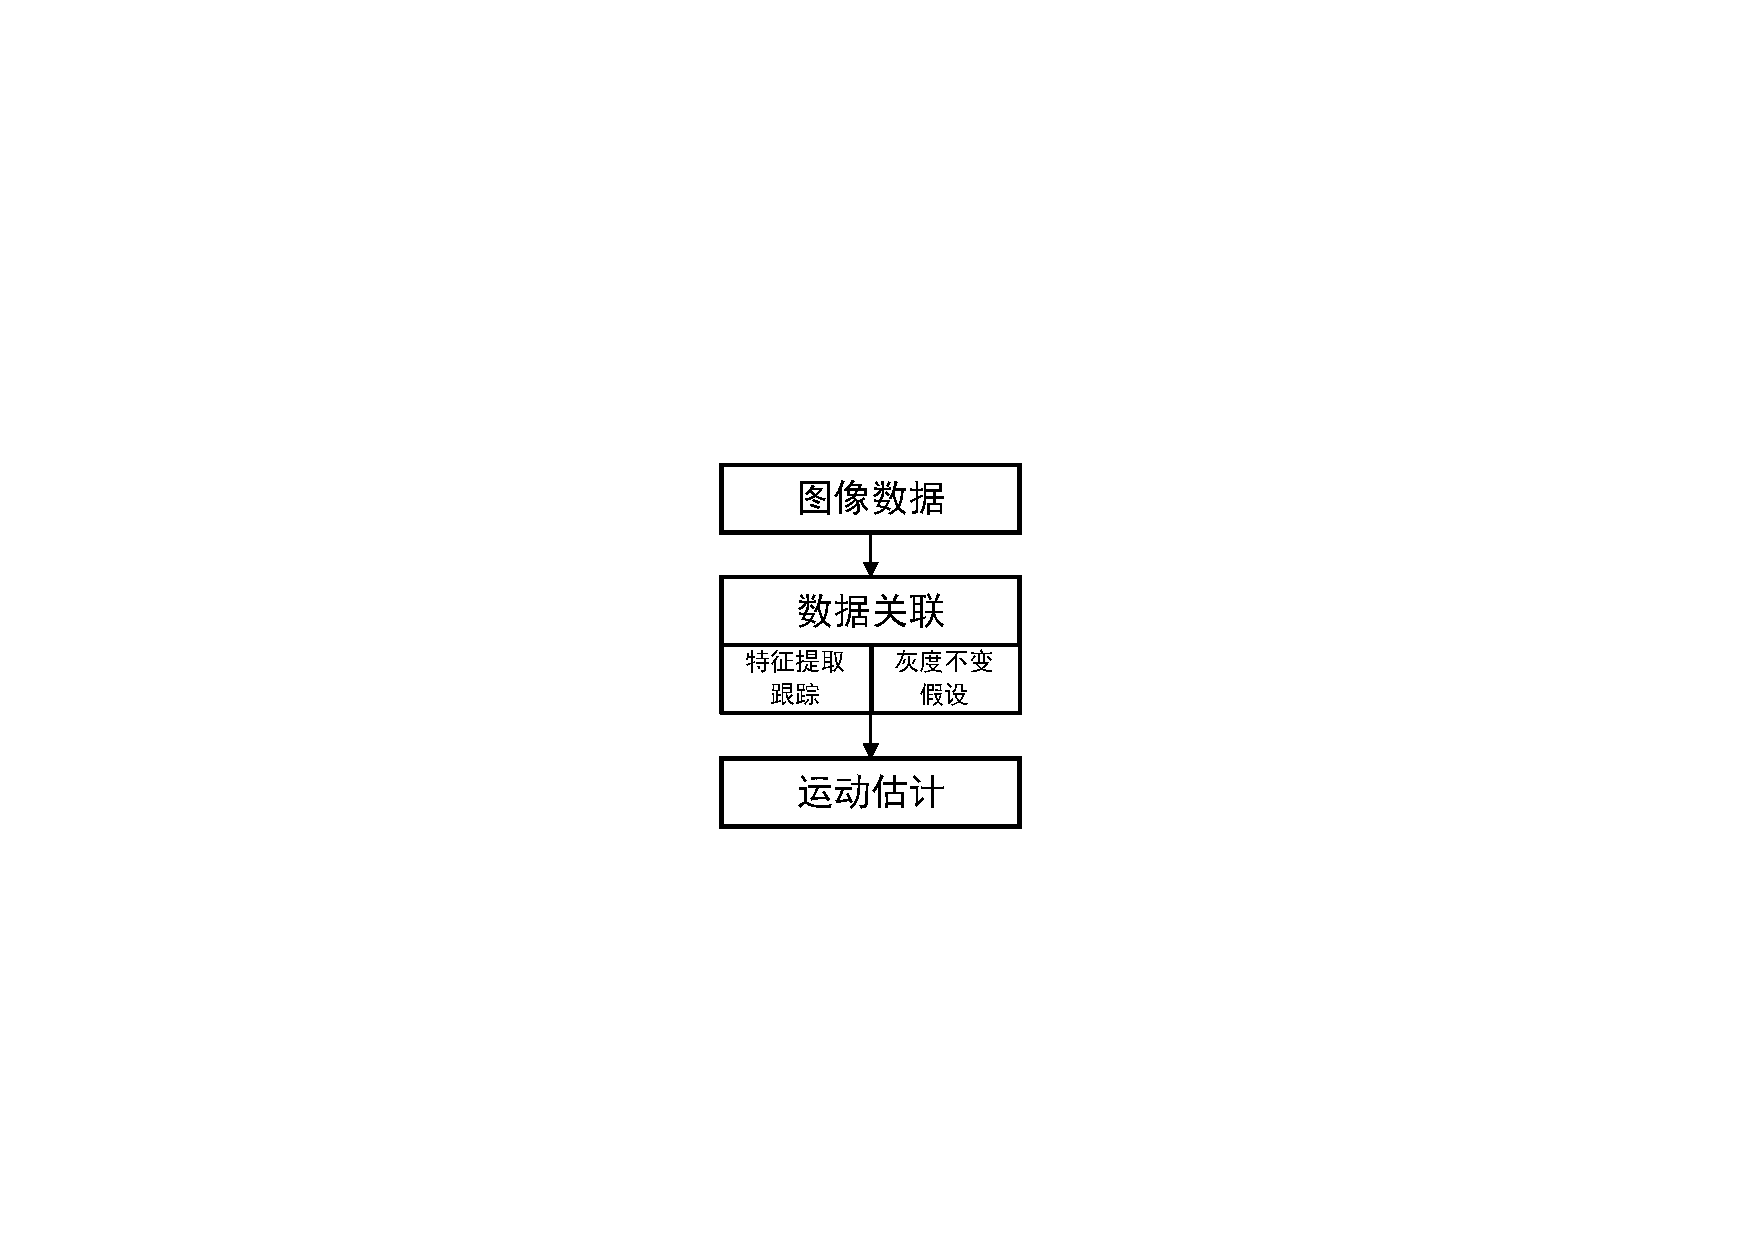
\includegraphics[scale=0.7,angle=-90]{figures/Fig3-2.pdf}
\caption{视觉里程计算法流程图}
\label{fig3.2}
\end{figure}
\vspace{-20pt}

视觉里程计得到的轨迹和地图,由于在运动估计时只考虑了帧间的信息,每次估计都带有一定的误差,串联的轨迹无可避免会出现累计漂移,这将导致无法得到全局一致的轨迹与地图。需要通过后端优化算法进行处理,估计运动和周围环境的不确定性,减小误差,提高轨迹和地图的精度。


%3.1.2
\subsection{后端优化}
SLAM后端优化将SLAM看作最大后验估计问题,且大都采用因子图的方式来表示变量之间的依赖关系\upcite{[3.2]}。一般的,假设状态变量为$\mathcal{X}$,变量$\mathcal{X}$包括无人机的轨迹和地图点的位置。传感器的测量值$Z=\lbrace z_k:k=1,\ldots ,m\rbrace$,且每个测量值可以表示为状态变量$\mathcal{X}$的函数,例如$z_k=h_k\left( \mathcal{X}_k \right)+\epsilon_k$,其中$\mathcal{X}_k \in \mathcal{X}$是$k$时刻的状态变量,$h_k(\cdot)$表示传感器的观测模型,$\epsilon_k$是随机观测误差。

最大后验估计通过计算后验概率$\mathds{P}\left(\mathcal{X} \vert Z\right)$取最大时对应的变量$\mathcal{X}^*$来估计状态变量$\mathcal{X}$的值
\begin{equation}
\label{equ3.1}
\mathcal{X}^* 
\doteq 
\argmax \limits_{\mathcal{X}} \mathds{P}\left(\mathcal{X} \vert Z\right) 
=
\argmax \limits_{\mathcal{X}}\mathds{P}\left(Z \vert \mathcal{X}  \right)\mathds{P}\left(\mathcal{X}\right)
\end{equation}
在公式\eqref{equ3.1}中$\mathds{P}\left(Z \vert \mathcal{X}  \right)$表示在状态变量$\mathcal{X}$确定情况下测量值$Z$的似然,$\mathds{P}\left(\mathcal{X}\right)$表示状态$\mathcal{X}$的先验概率。先验概率包括任何关于状态$\mathcal{X}$的先验信息,如果没有可用的先验信息,则$\mathds{P}\left(\mathcal{X}\right)$表示为一个常量,可以从优化过程中移除。在这种情况下,最大后验估计可以简化为极大似然估计。

假设测量值$Z=\lbrace z_k:k=1,\ldots ,m\rbrace$相互独立(测量噪声不相关),公式\eqref{equ3.1}可以表示为:
\begin{equation}
\label{equ3.2}
\mathcal{X}^* 
= 
\argmax \limits_{\mathcal{X}} \mathds{P}\left(\mathcal{X}\right) \prod \limits_{k=1}^{m} \mathds{P}\left(z_k \vert \mathcal{X}  \right)
=
\mathds{P}\left(\mathcal{X}\right) \prod \limits_{k=1}^{m} \mathds{P}\left(z_k \vert \mathcal{X}_k  \right)
\end{equation}
其中,等式右边的测量值$z_k$仅仅与状态变量$\mathcal{X}_k$有关。

公式\eqref{equ3.2}可以用因子图\upcite{[3.3]}表示,如图\ref{fig3.3}所示。状态变量作为节点(图中的$x_i,l_i,K$),似然$\mathds{P}\left(z_k \vert \mathcal{X}_k  \right)$和先验$\mathds{P}\left(\mathcal{X} \right)$作为因子(图中的黑色方框),描述了对节点的概率约束。因子图表示了第$k$个因子和对应状态变量$\mathcal{X}_k$依赖关系的图模型。因子图将SLAM问题可视化,便于理解。

\begin{figure}[h]
\centering
\includegraphics[scale=0.5,angle=-90]{figures/Fig3-3.pdf}
\caption{SLAM因子图}
\label{fig3.3}
\end{figure}
\vspace{-20pt}

为了更清楚的表示公式\eqref{equ3.2},假设观测模型的测量噪声$\epsilon_k$服从信息矩阵为$\Omega_k$的零偏高斯分布。测量值的似然可以表示为
\begin{equation}
\label{equ3.3}
\mathds{P}\left(z_k \vert \mathcal{X}_k  \right) \varpropto \exp ( -{1 \over 2} \left\| z_k -  h_k\left( \mathcal{X}_k \right) \right\|_{\Omega_k}^2 )
\end{equation}
其中$\left\| e \right\|_{\Omega}^2 = e^T \Omega e$。类似的,假设先验也服从高斯分布:
\begin{equation}
\label{equ3.4}
\mathds{P}\left( \mathcal{X}  \right) \varpropto \exp ( -{1 \over 2} \left\| z_0 - h_0\left(  \mathcal{X} \right)  \right\|_{\Omega_0}^2 )
\end{equation}
其中$h_0(\cdot)$表示观测模型,先验均值为$z_0$,信息矩阵为$\Omega_0$。由于最大后验与最小负对数后验等价,则公式\eqref{equ3.2}的最大后验估计可以表示为:
\begin{equation}
\label{equ3.5}
\mathcal{X}^* 
=
\argmin \limits_{\mathcal{X}} - \log \left( \mathds{P}\left(\mathcal{X}\right) \prod \limits_{k=1}^{m} \mathds{P}\left(z_k \vert \mathcal{X}_k  \right) \right)
=
\argmin \limits_{\mathcal{X}} \sum \limits_{k=0}^{m} -{1 \over 2} \left\|  z_k - h_k\left(   \mathcal{X}_k \right)  \right\|_{\Omega_k}^2
\end{equation}
公式\eqref{equ3.5}的形式是典型的非线性最小二乘问题,其中$h_k(\cdot)$是一个非线性函数。需要注意,公式\eqref{equ3.5}的前提是假设观测模型的观测噪声服从高斯分布,对于不同的观测噪声分布,将会得到不同的目标优化函数。例如,若观测噪声服从拉普拉斯分布,则公式\eqref{equ3.5}的平方$l_2$范数应变为$l_1$范数。另外,为了增加算法对于离群值的鲁棒性,通常使用鲁棒核函数\upcite{[3.4]}替换公式\eqref{equ3.5}中的平方$l_2$范数。

公式\eqref{equ3.5}的形式与SFM中的Bundle Adjustment(BA)问题相似,这是因为公式\eqref{equ3.5}与BA都是从最大后验估计出发推导得到的。但是,SLAM问题具有两个特点。首先,不同于SFM中的BA问题受限于几何模型约束,公式\eqref{equ3.5}适用于各种传感器模型。比如惯性传感器,GPS,轮式传感器等。其次,公式\eqref{equ3.5}是增量式的求解。

对于解决公式\eqref{equ3.5}的最小化问题,可通过连续线性化求解。例如高斯-牛顿法(G-N)和列文伯格-马夸尔特法(L-M)。高斯-牛顿方法从给定的初值$\hat{\mathcal{X}}$开始迭代,每次迭代时高斯-牛顿法估计公式\eqref{equ3.5}的最小值对应的状态增量
\begin{equation}
\label{equ3.6}
\delta_\mathcal{X}^* 
=
\argmin \limits_{\delta_\mathcal{X}} {1 \over 2} \sum \limits_{k=0}^{m} \left\| A_k\delta_\mathcal{X}-b_k \right\|_{\Omega_k}^2
=
\argmin \limits_{\delta_\mathcal{X}} {1 \over 2} \left\| A\delta_\mathcal{X}-b \right\|_{\Omega}^2
\end{equation}
其中公式\eqref{equ3.6}中的$\delta_\mathcal{X}$表示初始估计状态$\hat{\mathcal{X}}$的微小修正量;$A_k \doteq - {\partial h_k(\mathcal{X}) \over \partial \mathcal{X}} $是观测模型$h_k(\cdot)$关于$\mathcal{X}$的雅各比,$b_k \doteq z_k-h(\mathcal{X})$表示测量值与观测模型预测值之间的残差;公式\eqref{equ3.6}右边的矩阵$A$,$b$是由$A_k$,$b_k$组成的矩阵;$\Omega$是由观测噪声信息矩阵$\Omega_k$组成的对角块矩阵。

公式\eqref{equ3.6}对应的微小修正$\delta_\mathcal{X}^* $可以用下面的公式计算
\begin{equation}
\label{equ3.7}
\delta_\mathcal{X}^* = - \left( A^T \Omega^{-1} A \right)^{-1} A^T \Omega^{-1} b
\end{equation}
每次通过$\hat{\mathcal{X}} \leftarrow \hat{\mathcal{X}}+\delta_\mathcal{X}^*$迭代更新估计状态,矩阵$A^T \Omega^{-1} A$近似认为是Hessian矩阵。之前的推导过程中,我们假设$\mathcal{X}$属于向量空间。如果$\mathcal{X}$属于流形空间(如旋转矩阵),则高斯-牛顿法的形式保持不变,但是迭代更新方程$\hat{\mathcal{X}} \leftarrow \hat{\mathcal{X}}+\delta_\mathcal{X}$会被更合适的映射法则\upcite{[3.5]}取代。在机器人领域中,通常使用符号$\oplus$表示状态更新的映射关系,并且将状态的微小修正量$\delta_\mathcal{X}$定义在流形的切空间上,此时的更新方程为$\hat{\mathcal{X}}  \leftarrow \hat{\mathcal{X}} \oplus \delta_\mathcal{X}$。

现代SLAM算法最大的进步,在于认识到公式\eqref{equ3.7}中的雅各比矩阵$A$的稀疏性,而矩阵$A$的稀疏性是由于因子图内在的拓扑逻辑所决定的,利用矩阵稀疏性可以快速求解线性方程中状态的微小增量$\delta_\mathcal{X}^*$。此外,还可以设计增量式的求解方法,将更新后的状态变量作为新的观测值。当前主流SLAM后端优化库(如GTSAM,g2o,Ceres,iSAM,SLAM++)可以在几秒之内求解数以万计的状态变量。


%3.1.3
\subsection{回环检测}
上文介绍了SLAM的前端视觉里程计和后端优化:前端将传感器观测到的数据进行关联并将观测值抽象为适于后端估计的状态(轨迹,地图点位置);后端负责根据前端的结果对系统状态进行优化。然而,前端的视觉里程计只考虑时间关联性,之前测量产生的误差不可避免的会累计到下一时刻,产生累计误差,无法构建全局一致的轨迹和地图。后端优化虽然能够估计最大后验误差,但由于前端只提供了相邻时刻关键帧数据,无法消除累计误差。回环检测又称闭环检测,负责检测传感器是否经过同一个位置,通过增加与之前时刻的数据关联性约束,消除SLAM的轨迹与地图随时间漂移而产生的累计误差。回环检测对于SLAM算法意义重大,关系到SLAM算法估计的轨迹和地图在长时间运行中的准确性。另外,由于回环检测可以提供当前数据与历史数据的关联性,当SLAM算法前端跟踪丢失后,可以利用回环检测进行重定位,有效提高SLAM的精度和鲁棒性。

常用的回环检测方法有两种\upcite{[3.7]}:基于里程计的几何方法和基于外观的图像相似性。基于里程计的几何方法利用视觉里程计的位置信息,当发现运动到之前的某个位置附近时检测是否有回环关系。这是一种很直接的检测思路,但是由于存在累计误差,里程计无法正确的发现到底是否回到了曾经的某个位置。另一种方法是基于图像外观,这种方法和前端后端的输出无关,仅仅根据两幅图像之间的相似性进行判断。这种方法与累计误差完全无关,可以独立作为SLAM算法的一个模块,成为视觉SLAM中闭环检测的主流方法,应用于实际的SLAM系统中。


%3.2
\section{主流单目视觉SLAM算法研究}
近些年出现了许多优秀的单目SLAM算法,按照前端视觉里程计关联数据的方式不同分为基于直接法的SLAM和基于特征的SLAM两种。基于直接法的SLAM算法假设同一空间点的像素灰度值在不同图像中固定不变,估计最优位姿使得两幅图像经变换后灰度变化最小,完成前端的数据关联。基于特征的SLAM算法则提取图像中的特征,并在不同图像中对相同特征进行匹配,从而解算图像之间的相对运动,关联前端数据。本节主要研究两种代表性的单目SLAM算法:基于直接法的LSD-SLAM和基于特征的ORB-SLAM,分析对比两算法的原理、优势和不足,选择适用于无人机导航定位的单目SLAM算法,并针对其中存在的不足提出改进建议。

%3.2.1
\subsection{基于直接法的LSD-SLAM}

\subsubsection{算法概述}
LSD-SLAM是2014年慕尼黑工业大学的J.Engle等人提出的基于直接法的SLAM算法,无需计算图像特征点,通过直接法的像素关联估计运动状态,构建半稠密地图——半稠密是指估计灰度梯度明显区域的像素位置。该算法可以在大尺度环境下实时运行,利用半稠密像素关联和关键帧pose图优化构建全局一致的地图,关键帧间的pose图使用相似变换$\mathfrak{sim}(3)$代替$\mathfrak{se}(3)$,从而在后端优化中可以考虑不同场景的尺度变化,减小尺度漂移。LSD-SLAM的算法流程\upcite{[1.21]}如图\ref{fig3.4}所示。

\begin{figure}[h]
\centering
\includegraphics[scale=0.5,angle=-90]{figures/Fig3-4.pdf}
\caption{LSD-SLAM算法流程图}
\label{fig3.4}
\end{figure}
\vspace{-20pt}

LSD-SLAM算法主要分为三个部分:图像跟踪,深度估计和地图优化。图像跟踪部分获取相机采集的图像,利用上一帧的图像位姿作为初值,估计当前帧与关键帧的相对位姿$\xi \in \mathfrak{se}(3) $;深度估计部分根据当前帧情况,进行关键帧替换或位姿和像素逆深度优化。如果相机运动过快,则将新关键帧的地图点投影到临近关键帧进行初始化;如果当前帧被创建为新的关键帧,则之前关键帧的像素逆深度不再被优化。地图优化部分将之前的关键帧加入到全局地图中,使用尺度感知和图像相似变换关联来检测回环和尺度漂移,估计相邻关键帧之间的相似变换$\xi \in \mathfrak{sim}(3)$,优化关键帧的位姿和像素逆深度。

\subsubsection{数据关联与运动估计}
基于直接法的SLAM前提是灰度不变假设,即认为同一空间点的像素灰度值在不同图像中保持不变。直接法预先不知道像素之间的对应关系,而是通过最小化灰度误差来求解位姿变换和对应关系。如图\ref{fig3.5}所示,空间点$\boldsymbol{P}$的世界坐标为$[X,Y,Z]^T$,相机内参为$\boldsymbol{K}$,空间点$\boldsymbol{P}$在两幅图像中的对应像素坐标为$\boldsymbol{p_1},\boldsymbol{p_2}$。为了估计从图像1到图像2的相对位姿,以图像1的相机坐标系为参考系,假设图像2的位姿为$\boldsymbol{R},\boldsymbol{t}$,对应的李代数为$\boldsymbol{\xi} \in \mathfrak{se}(3) $。根据相机投影模型有:
\begin{equation}
\label{equ3.8}
\begin{aligned}
& \boldsymbol{p_1} = 
\begin{bmatrix}
u_1 \cr v_1 \cr 1 \cr 
\end{bmatrix}
={1 \over Z_1} \boldsymbol{K} \boldsymbol{P}
\\
& \boldsymbol{p_2} = 
\begin{bmatrix}
u_2 \cr v_2 \cr 1 \cr
\end{bmatrix}
={1 \over Z_2} \boldsymbol{K} ( \boldsymbol{R} \boldsymbol{P}+\boldsymbol{t}) = {1 \over Z_2} \boldsymbol{K} ( \exp (\boldsymbol{\xi}^{\wedge}) \boldsymbol{P})_{1:3}
\end{aligned}
\end{equation}
其中$Z_1$,$Z_2$是空间点$\boldsymbol{P}$在两个相机坐标系下的深度,$(\cdot)^{\wedge}$表示向量的反对称矩阵。由于位姿$\exp(\boldsymbol{\xi}^{\wedge})$与齐次坐标相乘,得到的结果只取前三个元素。

\begin{figure}[h]
\centering
\includegraphics[scale=0.3,angle=-90]{figures/Fig3-5.pdf}
\caption{直接法示意图}
\label{fig3.5}
\end{figure}
\vspace{-20pt}

直接法中只已知像素的灰度值,无法直接提供两幅图像的像素匹配,而是根据灰度不变假设估计相机间的相对位姿,最小化两幅图像像素灰度误差,也就是$P$点对应两个像素点的灰度误差。
\begin{equation}
\label{equ3.9}
\begin{aligned}
& e = I_1(\boldsymbol{p}_1) - I_2(\boldsymbol{p}_2) 
\\ 
& \min\limits_{\boldsymbol{\xi}} J(\boldsymbol{\xi}) = \Vert e \Vert ^2
\end{aligned}
\end{equation}
其中$I(\cdot)$表示图像像素灰度函数,目标优化函数为误差的二范数。对于空间中所有空间点,都应该满足灰度不变假设。若存在$N$个空间点$\boldsymbol{P}_i$,相机位姿估计问题可以表示为:
\begin{equation}
\label{equ3.10}
\min\limits_{\boldsymbol{\xi}} J(\boldsymbol{\xi}) = \sum\limits_{i=1}^N e_i^T e_i
\end{equation}
其中优化变量是相机位姿$\boldsymbol{\xi}$,为了得到最优解需要研究位姿$\boldsymbol{\xi}$变化对误差$e$的影响,即误差关于位姿的导数。使用李代数左乘扰动模型增加扰动$\exp( \delta \boldsymbol{\xi}^{\wedge})$,有:
\begin{equation}
\label{equ3.11}
\begin{aligned}
e(\boldsymbol{\xi}\oplus \delta \boldsymbol{\xi}) & = I_1\left({1 \over Z_1} \boldsymbol{K} \boldsymbol{P} \right) - I_2\left({1 \over Z_2} \boldsymbol{K} \exp (\delta \boldsymbol{\xi}^{\wedge}) \exp (\boldsymbol{\xi}^{\wedge}) \boldsymbol{P} \right)
\\
& \approx I_1\left( {1 \over Z_1} \boldsymbol{K} \boldsymbol{P} \right) - I_2 \left( {1 \over Z_2} \boldsymbol{K} (1+\delta \boldsymbol{\xi}^{\wedge}) \exp (\boldsymbol{\xi}^{\wedge}) \boldsymbol{P} \right)
\\
& = I_1\left( {1 \over Z_1} \boldsymbol{K} \boldsymbol{P} \right) - I_2 \left({1 \over Z_2} \boldsymbol{K} \exp (\boldsymbol{\xi}^{\wedge}) \boldsymbol{P}+ {1 \over Z_2} \boldsymbol{K} \delta \boldsymbol{\xi}^{\wedge} \exp (\boldsymbol{\xi}^{\wedge}) \boldsymbol{P} \right)
\end{aligned}
\end{equation}
记公式\eqref{equ3.11}中的$\boldsymbol{q} = \delta \boldsymbol{\xi}^{\wedge} \exp (\boldsymbol{\xi}^{\wedge}) \boldsymbol{P} $,$\boldsymbol{u}={1 \over Z_2} \boldsymbol{K} \boldsymbol{q}$,$\boldsymbol{q}$为$\boldsymbol{P}$点受到扰动后在图像2的相机坐标系下的坐标,$\boldsymbol{u}$为它的像素坐标。利用一阶泰勒近似,得到:
\begin{equation}
\label{equ3.12}
\begin{aligned}
e(\boldsymbol{\xi}\oplus \delta \boldsymbol{\xi}) &= I_1\left({1 \over Z_1} \boldsymbol{K} \boldsymbol{P} \right) - I_2 \left({1 \over Z_2} \boldsymbol{K} \exp (\boldsymbol{\xi}^{\wedge}) \boldsymbol{P}+ \boldsymbol{u} \right) 
\\ 
& \approx I_1\left({1 \over Z_1} \boldsymbol{K} \boldsymbol{P} \right) - I_2 \left({1 \over Z_2} \boldsymbol{K} \exp (\boldsymbol{\xi}^{\wedge}) \boldsymbol{P} \right) - {\partial I_2 \over \partial \boldsymbol{u}} {\partial \boldsymbol{u} \over \partial \boldsymbol{q}} {\partial \boldsymbol{q} \over \partial \delta \boldsymbol{\xi}} \delta \boldsymbol{\xi}
\\
& = e(\boldsymbol{\xi}) - {\partial I_2 \over \partial \boldsymbol{u}} {\partial \boldsymbol{u} \over \partial \boldsymbol{q}} {\partial \boldsymbol{q} \over \partial \delta \boldsymbol{\xi}} \delta \boldsymbol{\xi}
\end{aligned}
\end{equation}
在公式\eqref{equ3.12}中一阶泰勒展开的导数由链式法则分解为三项,$\partial I_2 / \partial \boldsymbol{u}$表示点$\boldsymbol{P}$在图像2中的像素灰度梯度;$\partial \boldsymbol{u} / \partial \boldsymbol{q}$表示相机投影方程关于相机坐标系下的三维点坐标的导数,假设$\boldsymbol{q} = \left[X_2,Y_2,Z_2 \right]^T$,其导数为:
\begin{equation}
\label{equ3.13}
{ \partial \boldsymbol{u} \over \partial \boldsymbol{q} } = 
\begin{bmatrix}
\partial u \over \partial X_2 & \partial u \over \partial Y_2 & \partial u \over \partial Z_2 \cr
\partial v \over \partial X_2 & \partial v \over \partial Y_2 & \partial v \over \partial Z_2 \cr
\end{bmatrix} = 
\begin{bmatrix}
f_x \over Z_2 & 0 & -f_x X_2 \over Z_2^2 \cr
0 & f_y \over Z_2 & - f_y Y_2 \over Z_2^2 \cr
\end{bmatrix}
\end{equation}
${\partial \boldsymbol{q} / \partial \delta \boldsymbol{\xi}}$表示图像2相机坐标系下的坐标对位姿的导数,有:
\begin{equation}
\label{equ3.14}
{\partial \boldsymbol{q} \over \partial \delta \boldsymbol{\xi}} = \left[\boldsymbol{I}_{3\times 3},-\boldsymbol{q}^{\wedge} \right]
\end{equation}
对于公式\eqref{equ3.10}位姿估计问题可以使用以上公式得到优化目标函数的雅各比矩阵,在给定初值后利用高斯-牛顿(G-N)或列文伯格-马夸尔特(L-M)方法迭代求解,估计相机帧间位姿,完成数据关联。




%3.2.2
\subsection{基于特征的ORB-SLAM}

\subsubsection{算法概述}
ORB-SLAM算法是Ra\'u l等人于2015年提出的基于特征的单目SLAM算法,是当前SLAM中最为完整和易用的SLAM系统。通过多线程保证整个算法实时运行,可应用于不同尺度大小的室内和室外场景,并且对于剧烈运动有较好的鲁棒性。整个系统围绕ORB特征\upcite{[3.8]},包括视觉里程计和回环检测中的ORB字典\upcite{[3.9]}。并对特征点进行优化,如在OpenCV特征提取基础上保证特征点均匀分布,宽松的关键帧建立机制和严苛的关键帧筛选机制,循环优化4遍相机位姿以得到更多的匹配。以上改进和优化使得ORB-SLAM具有很好的鲁棒性,代表了当前基于特征的SLAM算法的最高水平,ORB-SLAM算法结构\upcite{[1.20]}如图\ref{fig3.6}所示。

\begin{figure}[h]
\centering
\includegraphics[scale=0.5,angle=-90]{figures/Fig3-6.pdf}
\caption{ORB-SLAM算法流程图}
\label{fig3.6}
\end{figure}
\vspace{-20pt}

ORB-SLAM主要分为三部分,特征跟踪,局部地图和闭环检测。特征跟踪负责提取新图像的特征点,并与临近的关键帧匹配,估计当前帧的位姿并选择合适的帧作为新的关键帧;局部地图负责维护Covisibility图,通过求解BA问题来优化局部地图中关键帧位姿和地图点位置,剔除冗余的关键帧和地图点;闭环检测对全局地图与关键帧进行回环检测,维护一个pose图约束帧间位姿,消除累计误差。最后在每次回环完成后,独立进行一次全局BA,优化全部关键帧位姿和地图点位置,提高地图精度和一致性。


\subsubsection{特征提取与匹配}
图像是由灰度组成的矩阵,如果直接从矩阵层面考虑运动估计会非常困难,基于特征的SLAM算法从图像中选取一些代表性的特征。为了保证在相机运动之后特征点的稳定,特征点应该满足如下性质:
\begin{enumerate}[label={(\arabic*)}]
\item 可重复性:相同特征可以在不同的图像中被找到。
\item 可区别性:不同的特征有不同的表达。
\item 高效性:同一图像中,特征数量远小于像素数量。
\item 本地性:特征仅与小块图像区域相关。
\end{enumerate}

特征由关键点和描述子两部分组成。关键点指该特征在图像中的位置,有些关键点具有朝向、大小等信息;描述子通常由方向向量表示,按照人为设计的方式,描述关键点周围像素的信息,描述子的设计原则是相似的特征应该有相似的描述子。因此,当两个特征的描述子在向量空间上的距离接近时,可以认为是相同的特征。

ORB特征的关键点称为"Oriented FAST",FAST是一种图像角点\upcite{[3.10]},主要检测局部灰度变化明显的区域,提取速度快。ORB特征对原有的FAST特征点进行改进,添加了尺度和旋转不变性。旋转不变性通过构建尺度金字塔,并在金字塔每层检测角点来实现。旋转不变性则利用灰度质心法,以图像灰度值作为权重计算图像块质心,利用图像质心和几何中心设计方向向量保证特征旋转不变性;ORB特征的描述子为改进BRIEF描述子,BRIEF是一种二进制描述子\upcite{[3.11]},由0,1编码的向量表示关键点周围的两个像素的灰度大小关系。BRIEF使用随机选点的比较,速度快,存储方便,但是不具有旋转不变性。ORB特征在原有BRIEF描述子的基础上利用Oriented FAST关键点的方向信息,获取Steer BRIEF,使ORB特征描述子具有较好的旋转不变性。ORB特征相比于其他特征,如SHIFT、SURF特征,在保证精度和鲁棒性的前提下具有更好的计算速度和提取效率,适用于实时性要求较高的视觉SLAM算法。

\subsubsection{数据关联与运动估计}
在完成图像特征提取后,需要对图像间的相同特征进行匹配。特征匹配是SLAM算法中重要的一步,解决了SLAM的数据关联,确定了当前图像特征与之前图像特征的对应关系。考虑两个时刻的图像,假设在图像$I_t$中提取的特征点为$x_t^m,m=1,2,\cdots,M$,在图像$I_{t+1}$中提取到特征点为$x_{t+1}^n,n=1,2,\cdots,N$,最简单的方法是进行暴力匹配,对每个特征点$x_t^m$与所有的特征点$x_{t+1}^n$,测量两者描述子之间的距离,取最接近的作为匹配点。描述子距离表示描述子的相似程度,对于浮点类型的描述子可以使用欧氏距离,对于BRIEF这样的二进制描述子,一般使用汉明距——比较描述子不同位的个数。在特征匹配中,暴力匹配是最直接的方法,但当特征点数量较多,尤其在与地图进行匹配时,暴力匹配将花费很大的计算时间,无法满足SLAM算法实时性要求。ORB-SLAM引入恒速模型匹配特征,假设当前帧的运动与上一帧相同从而得到初始位姿,之后利用初始位姿将上一帧的特征或地图点投影到当前帧就近匹配,极大的提高了匹配速度。

当完成特征点匹配后,需要根据特征匹配结果估计相机运动。首先在初始化阶段,由于单目只知道2D像素坐标信息,需要根据对极几何解决初始位姿估计,对极几何描述了匹配特征点之间的几何关系,如图\ref{fig3.7}所示。

\begin{figure}[h]
\centering
\includegraphics[scale=0.3,angle=-90]{figures/Fig3-7.pdf}
\caption{对极几何约束}
\label{fig3.7}
\end{figure}
\vspace{-20pt}

假设第一帧到第二帧的相对运动为$\boldsymbol{R}$,$\boldsymbol{t}$,两个相机中心分别为$O_1$,$O_2$。考虑空间点$\boldsymbol{P}=[X,Y,Z]^T$在两帧图像上的对应特征点$\boldsymbol{p}_1$,$\boldsymbol{p}_2$。根据相机投影模型,有:
\begin{equation}
\label{equ3.15}
s_1 \boldsymbol{p}_1 = \boldsymbol{K} \boldsymbol{P}, \ \ \ 
s_2 \boldsymbol{p}_2 = \boldsymbol{K} (\boldsymbol{R} \boldsymbol{P}+\boldsymbol{t})
\end{equation}
在公式\eqref{equ3.15}中$\boldsymbol{K}$表示相机内参,$s_1$,$s_2$表示在两相机坐标系下的空间点深度,空间点坐标使用齐次坐标表示,现在取
\begin{equation}
\label{equ3.16}
\boldsymbol{x}_1 = \boldsymbol{K}^{-1} \boldsymbol{p}_1, \ \ \ 
\boldsymbol{x}_2 = \boldsymbol{K}^{-1} \boldsymbol{p}_2
\end{equation}
将方程\eqref{equ3.16}代入方程\eqref{equ3.15}中,可以得到
\begin{equation}
\label{equ3.17}
s_2 \boldsymbol{x}_2 = s_1 \boldsymbol{R} \boldsymbol{x}_1 + \boldsymbol{t}
\end{equation}
将方程\eqref{equ3.17}两侧同时左乘$\boldsymbol{t}$的反对称矩阵$\boldsymbol{t}^{\wedge}$,再左乘$\boldsymbol{x}_2^T$,有:
\begin{equation}
\label{equ3.18}
\boldsymbol{x}_2^T  \boldsymbol{t}^{\wedge}  \boldsymbol{R} \boldsymbol{x}_1 = \boldsymbol{x}_2^T \boldsymbol{t}^{\wedge} \boldsymbol{x}_2 = 0
\end{equation}
重新代入$\boldsymbol{p}_1$,$\boldsymbol{p}_2$可以得到:
\begin{equation}
\label{equ3.19}
\boldsymbol{p}_2^T \boldsymbol{K}^{-T} \boldsymbol{t}^{\wedge}  \boldsymbol{R} \boldsymbol{K}^{-1} \boldsymbol{p}_1  = 0
\end{equation}
公式\eqref{equ3.18}, \eqref{equ3.19}都称为对极约束,同时包含了旋转和平移信息。两方程中间的矩阵分别记为本质矩阵$\boldsymbol{E} = \boldsymbol{t}^{\wedge}  \boldsymbol{R} $和基本矩阵$\boldsymbol{F} = \boldsymbol{K}^{-T} \boldsymbol{t}^{\wedge}  \boldsymbol{R} \boldsymbol{K}^{-1}$。通过分解以上两个矩阵,可以获得两帧图像的相对运动。之后对两帧关键帧的匹配特征进行三角化,在公式\eqref{equ3.17}等号两边同时左乘$\boldsymbol{x}_1^{\wedge}$可以得到
\begin{equation}
\label{equ3.20}
s_2 \boldsymbol{x}_1^{\wedge} \boldsymbol{R} \boldsymbol{x}_2 + \boldsymbol{x}_1^{\wedge} \boldsymbol{t} = s_1 \boldsymbol{x}_1^{\wedge} \boldsymbol{x}_1 = 0
\end{equation}
通过求解方程\eqref{equ3.20}可以直接得到$s_2$,根据求得结果可以很容易得到$s_1$,获得初始地图点云。需要注意的是,由于单目无法提供深度信息,以上估计的位姿和地图点无法确定准确的尺度,一般将初始化地图点深度均值归一化为1。

在ORB-SLAM完成初始化得到初始关键帧和地图后,对于后续的帧图像,利用恒速模型将上一帧中的地图点投影到当前帧,在阈值范围内搜索匹配特征,通过最小化重投影误差求解当前帧的位姿。考虑$n$个三维空间点$\boldsymbol{P}_i$和他们的投影$\boldsymbol{p}_i$,当前帧的位姿$\boldsymbol{R}$,$\boldsymbol{t}$用李代数$\boldsymbol{\xi}$表示。假设空间点坐标为$\boldsymbol{P}_i=[X_i,Y_i,Z_i]^T$,其投影的像素坐标为$\boldsymbol{p}_i = [u_i,v_i]^T$,根据相机投影模型有
\begin{equation}
\label{equ3.21}
s_i
\begin{bmatrix}
u_i \cr v_i \cr 1\cr 
\end{bmatrix}
=
\boldsymbol{K} \exp\left( \boldsymbol{\xi}^{\wedge} \right)
\begin{bmatrix}
X_i \cr Y_i \cr Z_i \cr 1 \cr
\end{bmatrix}
\end{equation}
方程\eqref{equ3.21}表示由关键帧位姿预测的地图点云投影像素位置,由于相机位姿不准确且系统存在观测误差,观测到的匹配点$\boldsymbol{p}_i$与预测值存在误差,可以构建BA问题优化相机位姿,优化函数为。
\begin{equation}
\label{equ3.22}
\boldsymbol{\xi}^* = \argmin\limits_{\boldsymbol{\xi}} {1 \over 2} \sum\limits_{i=1}^n  \left \Vert \boldsymbol{p}_i - {1 \over s_i} \boldsymbol{K} \exp\left( \boldsymbol{\xi}^{\wedge} \right) \boldsymbol{P}_i  \right \Vert_2^2
\end{equation}
方程\eqref{equ3.22}中的误差称为重投影误差,通过高斯-牛顿(G-N)或列文伯格-马夸尔特(L-M)等优化方法可以很容易的求解位姿。

%3.3
\section{两种SLAM算法比较}
上节针对主流的单目SLAM算法原理进行了分析,本节将在数据集上对两SLAM算法进行实验和比较,对比两种算法的定位精度、鲁棒性和地图重建效果,根据实验结果分析两种SLAM算法的优缺点。结合无人机的运动特性选择合适的视觉SLAM导航定位方法,并针对其存在的问题提出改进方案。

\subsubsection{定位精度}
TUM RGB-D数据集\upcite{[3.12]}包含了多种室内场景的图像序列,并且每个序列通过外部视觉捕捉系统提供了准确的运动轨迹,适用于评估视觉SLAM算法的定位精度,数据集场景见附录\ref{DataSets}。对单目SLAM算法进行实验测试时,只使用TUM数据集的RGB图像。对于单目SLAM输出的轨迹结果,通过$\mathfrak{sim}(3)$相似变换进行轨迹对齐,比较关键帧轨迹均方根误差(RMSE),误差定义为:
\begin{equation}
\label{equ3.23}
\begin{aligned}
\boldsymbol{F}_i &\doteq \boldsymbol{Q}_i^{-1} S \boldsymbol{P}_i
\\ 
R\!M\!S\!E(\boldsymbol{F}) &\doteq \left( {1 \over n} \sum\limits_{i=1}^n \left \Vert trans(\boldsymbol{F}_i) \right \Vert^2 \right)^{1 \over 2} 
\end{aligned}
\end{equation}
其中$\boldsymbol{Q}_i$表示真值轨迹第$i$时刻的位置,$\boldsymbol{P}_i$表示估计轨迹第$i$时刻的位置,$\boldsymbol{S}$表示用于对齐轨迹的$\mathfrak{sim}(3)$相似变换,实验结果如下表\ref{tab3.1}所示。

\vspace{-10pt}
\begin{table}[h]		%表格环境
% \multicolumn是跨列功能,第一个参数2,表示跨两列,第二个参数c|,表示文字置中,并在栏位右边画一条直线框,最后一个参数即是要填入的文字
%\multirow是跨行功能,第一个参数2,表示跨两行,第二个参数*,表示系统自动调整文字,最后一个参数即是要填入的文字
%\newcommand{\tabincell}[2]{\begin{tabular}{@{}#1@{}}#2\end{tabular}}		%单元格内容强制换行
\renewcommand\arraystretch{1.5}		%增加行间距
\centering
\caption{TUM数据集单目SLAM算法轨迹定位精度}   % 表格标题,在表格内容之前
\label{tab3.1}
	\begin{tabular*}{0.9\textwidth}{@{\extracolsep{\fill}}ccc}  %生成行和列的表格
	%\begin{tabular}{p{2cm}p{1.5cm}p{1.5cm}p{1.5cm}}	
	
	\toprule
	
	\multicolumn{1}{c}{\multirow{2}{*}{Seq.}} &
	\multicolumn{2} {c} {\bfseries\tabincell{c} {关键帧轨迹均方根误差 RMSE(cm)}} \\
	\cline{2-3}								%在上一行下面,2-4列画横线
	\multicolumn{1}{c}{}&
	\multicolumn{1}{c}{ORB-SLAM}	&
	\multicolumn{1}{c}{LSD-SLAM}	\\	
	
	\midrule
	
	\multicolumn{1}{c}{fr1/xyz}		&
	\multicolumn{1}{c}{0.90}		&
	\multicolumn{1}{c}{9.00}		\\
	
	\multicolumn{1}{c}{fr2/xyz}		&
	\multicolumn{1}{c}{0.30}		&
	\multicolumn{1}{c}{2.15}		\\
	
	\multicolumn{1}{c}{fr1/desk}	&
	\multicolumn{1}{c}{1.69}		&
	\multicolumn{1}{c}{10.65}		\\
	
	\multicolumn{1}{c}{fr2/desk}	&
	\multicolumn{1}{c}{0.88}		&
	\multicolumn{1}{c}{4.57}		\\
	
	\multicolumn{1}{c}{fr2/desk\_ person}	&
	\multicolumn{1}{c}{0.63}		&
	\multicolumn{1}{c}{31.73}		\\
	
	\multicolumn{1}{c}{fr3/long\_ office}	&
	\multicolumn{1}{c}{3.45}		&
	\multicolumn{1}{c}{38.53}		\\

	\multicolumn{1}{c}{fr3/sit\_ xyz}	&
	\multicolumn{1}{c}{0.79}		&
	\multicolumn{1}{c}{7.73}		\\	
	
	\multicolumn{1}{c}{fr3/walk\_ halfsph}	&
	\multicolumn{1}{c}{1.74}		&
	\multicolumn{1}{c}{$\boldsymbol{X}$}		\\	
	\bottomrule
	
	\end{tabular*}
\end{table}
表\ref{tab3.1}是连续测试五次取均值的结果,$\boldsymbol{X}$表示运行过程中出现丢失无法完成整个图像序列。根据表\ref{tab3.1}的实验结果可以发现,ORB-SLAM算法的定位精度高于LSD-SLAM,主要原因可能是:(1)基于直接法的LSD-SLAM遵从灰度不变假设,对于相机内参和曝光非常敏感,而且直接法SLAM在相机运动过快时无法准确估计位姿;而基于特征的ORB-SLAM使用特征提取与匹配的方法关联数据,对传感器参数变化较为鲁棒,并且在快速运动时不易丢失。(2)基于直接法的LSD-SLAM计算复杂度较大,无法多次优化关键帧位姿。且LSD-SLAM将关键帧位姿与地图点的联合优化简化为pose图优化,影响了定位精度。

\subsubsection{地图重建效果}
选择TUM数据集中具有代表性的fr2/xyz,fr2/desk,fr3/long\_ office场景对比重构效果,实验结果如下图所示。
\begin{figure}[h]
\centering
	\subfigure[LSD-SLAM]
    {
		\includegraphics[scale=.24]{figures/Fig3.8_a.png}
	}
	\subfigure[ORB-SLAM]
    {	
		\includegraphics[scale=.3]{figures/Fig3.8_b.png}
	}
\caption{fr2/xyz场景}
\label{fig3.8}
\end{figure}

\begin{figure}[h]
\centering
	\subfigure[LSD-SLAM]
    {
		\includegraphics[scale=.15]{figures/Fig3.9_a.png}
	}
	\subfigure[ORB-SLAM]
    {	
		\includegraphics[scale=.3]{figures/Fig3.9_b.png}
	}
\caption{fr2/desk场景}
\label{fig3.9}
\end{figure}
\vspace{-0pt}

\begin{figure}[h]
\centering
	\subfigure[LSD-SLAM]
    {
		\includegraphics[scale=.25]{figures/Fig3.10_a.png}
	}
	\subfigure[ORB-SLAM]
    {	
		\includegraphics[scale=.21]{figures/Fig3.10_b.png}
	}
\caption{fr3/long\_ office场景}
\label{fig3.10}
\end{figure}
\vspace{-20pt}

通过对比重建结果可以发现,基于直接法的LSD-SLAM可以重构环境的半稠密地图,通过地图可以进行目标识别,避障与路径规划等其他任务;而基于特征的ORB-SLAM只能恢复环境的稀疏点云地图,无法提供丰富的环境信息。造成这样结果的原因在于:基于特征的SLAM算法只三角化图像的特征点,考虑到特征点的数量远低于像素数量,因而无法提供丰富的环境信息。直接法SLAM关联灰度变化明显区域的像素,而灰度变化明显的像素一般为物体边缘,因而可以重构环境的半稠密地图。

%3.4
\section{本章小结}
本章介绍了视觉SLAM的算法框架、理论原理和分类,从定位精度,鲁棒性和地图重构三个方面比较了基于直接法的LSD-SLAM和基于特征的ORB-SLAM。实验结果表明,相比于基于直接法的LSD-SLAM,基于特征的ORB-SLAM具有较好的光度不变性和视角不变性,可以在宽基线下稳定匹配特征,对于快速运动鲁棒性好,适宜作为无人机的导航定位系统。但其存在两个问题,首先,基于特征的ORB-SLAM重建地图为稀疏点云图,无法为无人机避障与路径规划等后续任务提供丰富的环境信息;另外,由于单目相机无法提供深度信息,因而估计得到的轨迹与地图尺度不确定。针对ORB-SLAM算法存在的问题,第四章研究基于特征的单目半稠密SLAM算法,解决稀疏点云地图环境信息不足的问题;第五章研究基于IMU预积分的惯性-视觉SLAM算法,解决单目SLAM尺度不确定问题。通过以上改进,使得本文研究的单目SLAM算法具有准确的尺度,较高的定位精度和丰富的环境信息,满足无人机导航定位的需要。



%%==================================================
%% chapter04.tex for BIT Master Thesis
%% modified by yang yating
%% version: 0.1
%% last update: Dec 25th, 2016

%% modified by Meng Chao
%% version: 0.2
%% last update: May 29th, 2017
%%==================================================
\chapter{基于特征的单目半稠密SLAM算法}
\label{chap:Semi-Dense}

针对基于特征的ORB-SLAM算法重构地图稀疏,无法用于避障和路径规划的问题。本章在原有算法的基础上,参考直接法SLAM半稠密地图重建原理,研究一种基于特征的单目半稠密SLAM算法。不同于直接法SLAM中使用连续多帧对关键帧逆深度进行滤波的做法,本文使用经过局部BA(Local BA)和回环pose图优化后的关键帧进行极线搜索,在保证定位精度的基础上重构环境的半稠密地图。本章研究的基于特征的单目半稠密SLAM算法主要包括5个部分,立体搜索约束,极线搜索,逆深度假设融合,帧内逆深度假设一致性检验和帧间逆深度假设一致性检验,算法流程如图\ref{fig4.1}所示。具体步骤如下:
\begin{enumerate}[label={(\arabic*)}]

\item 对选取的关键帧$K_i$,提取图像中像素灰度梯度满足阈值的像素点,在临近的$N$个关键帧中进行极线搜索,得到像素的逆深度假设。

\item 考虑到图像在观测过程中存在噪声、视差过小和二义性等问题,假设像素逆深度服从高斯分布\upcite{[4.1]},并认为相机关键帧的位姿是准确的,不考虑位姿的不确定性。

\item 由于关键帧之间的极线搜索是在宽基线条件下进行,搜索范围较大,需要考虑匹配过程中的误匹配。除考虑增加更多像素匹配约束外,采用高斯分布表示逆深度图中像素$p$的逆深度假设$N(\rho_p, \sigma_{\rho_p}^2)$,通过融合一致的逆深度假设降低误匹配的影响。

\item 对关键帧逆深度图中的像素逆深度进行融合,并且通过帧内逆深度假设一致性检验剔除与临近像素逆深度不一致的像素。

\item 完成当前关键帧和其相邻关键帧的逆深度假设计算后,对当前关键帧和相邻关键帧的像素逆深度进行一致性检验,剔除不一致的像素逆深度,并通过最小化深度误差优化像素深度。

\end{enumerate}

本章研究的基于特征的单目半稠密SLAM算法是在宽基线条件下进行极线搜索,容易导致误匹配产生离群值影响重构效果。因而相比于直接法SLAM,进行极线搜索时除考虑灰度梯度大小和方向的匹配外,还应进行逆深度假设融合和帧内与帧间逆深度假设一致性检验,剔除宽基线极线搜索的误匹配点,从而提高重构效果。

\begin{figure}[h]
\centering
\includegraphics[scale=0.4,angle=-90]{figures/Fig4-1.pdf}
\caption{基于特征的半稠密单目SLAM算法流程图}
\label{fig4.1}
\end{figure}





% 4.1
\section{立体搜索约束}
基于特征的单目SLAM算法可以通过特征匹配与跟踪,提供准确的相机位姿$R,t$, 用于像素间的块匹配进而得到像素逆深度假设。由于已知当前关键帧ORB特征点的深度信息,可以估计当前关键帧的最大逆深度$\rho_{max}$, 最小逆深度$\rho_{min}$和像素逆深度的先验信息$N\left( \rho_0,\sigma_{\rho_0}^2  \right)$,其中$\rho_{max}=\rho_0+2\sigma_{\rho_0}$,$\rho_{min}=\rho_0-2\sigma_{\rho_0}$。另外,通过Covisibility图可以获得与当前关键帧$K_i$具有最多共视关系的前$N$个关键帧的集合$K$,从而完成关键帧间的立体搜索。在进行立体搜索求解当前关键帧的逆深度假设前,进行延时处理。一方面可以避免由于局部BA导致的Covisibility图结构变化;另一方面可以引入之后时刻的关键帧,提高重建效果。


%4.2
\section{极线搜索}
对于当前关键帧$K_i$中像素梯度的模大于$\lambda_G$的像素$p$,会在关键帧$K_j \in K$的极线$l_j$上$\left[ \rho_{min}, \rho_{max} \right]$范围内进行搜索,寻找匹配的像素点,如图\ref{fig4.2}所示。极线利用基本矩阵$F_{ji}$求得,极线搜索方程为:

\begin{equation}
\label{equ4.1}
x_j^T F_{ji}x_p = x^T_jl_j=0 \  \rightarrow \  v_j = m \cdot u_j+n
\end{equation}


\begin{figure}
\centering
\includegraphics[scale=0.2,angle=-90]{figures/Fig4-2.pdf}
\caption{极线搜索}
\label{fig4.2}
\end{figure}



不同于直接法SLAM中的窄极线匹配,本章的极线搜索是在宽基线下进行的,因而除了像素块匹配外,需要加入更多约束,除比较像素灰度$I$之外,还应考虑像素梯度的模$G$和梯度方向$\Uptheta$,从而在极线$l_j$上找到合适的像素匹配。根据以下约束\upcite{[4.2]}, 排除$l_j$极线上不满足条件的像素。


\begin{enumerate}[label={(\arabic*)}]

\item 关键帧$K_j \in K$上的匹配像素$p_j$应位于图像像素梯度大的区域,像素梯度应大于阈值,$G(u_j)> \lambda_G$。

\item 考虑到匹配的二义性与沿极线方向的像素梯度有关,因而匹配像素的梯度方向不能与极线方向垂直,满足$\vert \Uptheta(u_j)-\Uptheta_L \pm \pi \vert < \lambda_L$,其中$\Uptheta_L$表示基线方向。

\item 匹配像素$p_j$与$p$的梯度方向应该相近,满足$\vert \Uptheta(u_j)-(\Uptheta_L \pm \Delta \theta_{j,i}) \vert < \lambda_\theta $,其中$\Delta \theta_{j,i}$表示两帧图像之间的旋转角度。

\end{enumerate}
以上匹配约束可以剔除关键帧$K_j \in K$极线$l_j$上的大部分像素点,剩余的为关键帧$K_i$中的像素$p$可能的匹配点。为了比较两个像素点的相似性, 定义像素相似误差函数$e(u_j)$:
\begin{equation}
\label{equ4.2}
\begin{aligned}
& e(u_j) = {r_I^2 \over \sigma_I^2} + {r_G^2 \over \sigma_G^2} \\ 
& r_I = I_p-I(u_j),\  r_G = G_p-G(u_j)
\end{aligned}
\end{equation}
其中$r_I$和$r_G$表示像素间的灰度和梯度误差,$\sigma_I$和$\sigma_G$表示像素灰度和梯度的标准差。由于像素梯度是根据灰度计算得到,若利用施密特算子$\triangledown$计算梯度, 则像素灰度与梯度的误差具有相关性,
$\sigma_G^2=\theta \sigma_I^2$ , $ \theta = 0.23$,则公式\eqref{equ4.2}可以简化为:
\begin{equation}
\label{equ4.3}
 e(u_j) = \left( {r_I^2}+{1 \over \theta} r_G^2 \right) {1 \over \sigma_I^2}
\end{equation} 

使相似误差函数最小的像素$u_0$为像素$p$的匹配像素, 其灰度误差和梯度误差为$r_{I_0}$、$r_{G_0}$,相似误差函数的导数为
\begin{equation}
\label{equ4.4}
{\partial e \over \partial u_j } = -{ -2(r_I g+ { 1 \over \theta} r_G q )  \over \sigma_I^2 }
\end{equation}
其中$g$表示灰度梯度的模,$q$表示灰度梯度导数的模,方向与极线相同。
\begin{equation}
\label{equ4.5}
\begin{aligned}
& g \approx { {I(u_j+1) - I(u_j-1)} \over 2 } \\
& q \approx { {G(u_j+1) - G(u_j-1)} \over 2 } 
\end{aligned}
\end{equation}

令公式\eqref{equ4.4}等于$0$可以得到匹配像素$u_0$,实际情况下像素$u_0$是沿极线以单位像素为步长搜索得到的整数坐标像素,而公式\eqref{equ4.4}的解不一定为整数。设公式\eqref{equ4.4}的解为$u_0^*=u_0+\Delta u$,对方程\eqref{equ4.2}中的相似误差函数进行一阶泰勒展开,带入公式\eqref{equ4.4}并令其等于$0$,可以得到
\begin{equation}
\label{equ4.6}
\Delta u = {{ r_I(u_0) g(u_0)+ {1 \over \theta} r_G(u_0)q(u_0) } \over {g^2(u_0)+ { 1 \over \theta} q^2(u_0)}}
\end{equation}
匹配像素的亚像素精度为
\begin{equation}
\label{equ4.7}
u_0^* = u_0 + {{ r_I(u_0) g(u_0)+ {1 \over \theta} r_G(u_0)q(u_0) } \over {g^2(u_0)+ { 1 \over \theta} q^2(u_0)}}
\end{equation}
根据误差传递理论,可以得到匹配像素$u_0^*$的不确定性。
\begin{equation}
\label{equ4.8}
\sigma_{u_0^*}^2 = \left \vert { \partial u^* \over \partial r_I(u_0) }  \right \vert \sigma_I^2 + \left \vert { \partial u^* \over \partial r_G(u_0) }  \right \vert \sigma_G^2 = { \sigma_I^2 \over g^2(u_0) + {1 \over \theta} q^2(u_0) }
\end{equation}
根据像素不确定性可以知道,沿极线方向像素灰度梯度和像素灰度梯度导数的模越大,匹配的可靠性越高。

为了得到匹配像素的逆深度假设不确定性,需要计算当前关键帧$K_i$中像素$p$的逆深度$\rho_p$。对匹配像素进行三角化,有$s_jX_j = s_pR_{ji}X_p+t_{ji}, \  X_j = K^{-1}P_j, X_p = K^{-1}P_p$,可以得到像素逆深度为
\begin{equation}
\label{equ4.9}
\rho_p(u_j) = { r_z^{ji} X_p (u_j-c_x) - f_x r_x^{ji} X_p  \over - t_z^{ji}(u_j-c_x)+f_x t_x^{ji} }
\end{equation}
其中$r_x^{ji}$,$r_z^{ji}$表示两帧间的旋转矩阵$R_{ji}$的第一行和第三行,$t_x^{ji}$,$t_z^{ji}$表示两帧间的平移向量$t_{ji}$的第一个和第三个元素;$f_x$、$c_x$是相机内参;$\rho_p = { 1 \over s_p}$,$P_j= \left [ u_j, v_j, 1 \right ] ^T$,利用方程\eqref{equ4.9}可以得到像素$p$的匹配像素$p_j$的逆深度假设$N(\rho_j, \sigma_{\rho_j}^2)$。
\begin{equation}
\label{equ4.10}
\begin{aligned}
 \rho_j &= \rho_p(u_0^*) \\ 
 \sigma_{\rho_j} &= max \left( \left \vert  \rho_p(u_0^*+\sigma_{u_0^*})-\rho_j \right \vert , \  \left \vert  \rho_p(u_0^*-\sigma_{u_0^*})-\rho_j \right \vert \right)
\end{aligned}
\end{equation}

在以上的逆深度假设不确定性的推导过程中,并没有像基于直接法SLAM一样引入帧间微小运动假设,因而本算法的逆深度假设不确定性具有一般性。


%4.3
\section{逆深度假设融合}
根据4.2节中的极线搜索方法,每个像素可以得到一组逆深度假设。由于存在极线像素逆深度立体搜索约束,且极线上匹配的像素需满足之前提到的像素匹配约束,因而逆深度假设的个数可能不足$N$个。另外,由于像素的相似性和遮挡,以上逆深度假设存在离群值。为了验证像素逆深度假设,在像素的一组逆深度假设中至少应该存在$\lambda_N$个一致假设。利用$\chi^2$假设检验(置信区间$95\%$,自由度2),验证两个逆深度假设分布的一致性。
\begin{equation}
\label{equ4.11}
{ (\rho_a - \rho_b)^2 \over \sigma_a^2 }+{ (\rho_b - \rho_a)^2 \over \sigma_b^2} < 5.991
\end{equation}

每次从像素的一组逆深度假设中选取一个,与其他逆深度假设进行一致性检验,若与其一致的逆深度假设数量超过$\lambda_N$个,则对该组逆深度按照公式\eqref{equ4.12}进行融合\upcite{[4.3]},像素$p$融合后的逆深度假设服从$N(\rho_p,\sigma_{\rho_p}^2)$,其中$n$表示通过检验的逆深度假设数量。
\begin{equation}
\label{equ4.12}
\rho_p = { {\sum\limits_n {1 \over \sigma_{\rho_j}^2} \rho_j } \over \sum\limits_n {1 \over \sigma_{\rho_j}^2}  }, \ 
\sigma_{\rho_p}^2 = {1 \over  \sum\limits_n { 1 \over \sigma_{\rho_j}^2}  }
\end{equation}


%4.4
\section{帧内逆深度假设一致性检验}
在完成当前关键帧$K_i$中像素的逆深度假设计算和融合后,需要对帧内所有逆深度假设进行一致性检验,用于剔除像素逆深度假设中的离群值。首先,通过公式\eqref{equ4.11}检验某像素和它临近的8个像素点的逆深度假设的一致性,若一致的逆深度假设数量多于2个,则保留该像素点的逆深度假设,否则剔除。若保留该像素,其逆深度根据公式\eqref{equ4.12}进行融合,不确定性为所有参与逆深度假设检验的像素中的最小不确定性。对于处于像素灰度变化明显区域但没有逆深度假设的像素点,若在该像素周围至少有两个逆深度假设一致的像素,则给该像素点添加逆深度假设,逆深度为附近一致逆深度假设的逆深度均值,不确定性是附近一致逆深度假设中的最小值,该方法可以增加地图重建的稠密性,起到平滑地图的作用。

%4.5
\section{帧间逆深度假设一致性检验}
在当前关键帧$K_i$的$N$个临近关键帧的像素逆深度全部计算完成后,对关键帧$K_i$中像素的逆深度假设进行帧间一致性检验。对于关键帧$K_i$中的像素$p$对应的逆深度$\rho_p$,将其投影到$K_i$临近的关键帧$K_j \in K$中,并计算像素$p$在关键帧$K_j \in K$中对应点的逆深度:
\begin{equation}
\label{equ4.13}
\begin{aligned}
& x_j = K R_{ji} {1 \over \rho_p} X_p + Kt_{ji} \\ 
& \rho_j = { \rho_p \over r_z^{ji}X_p+\rho_p t_z^{ji} }
\end{aligned}
\end{equation}
其中$x_{j}$表示关键帧$K_i$中的像素$p$在$K_j \in K$中投影点的像素坐标。若$x_j$的像素坐标不是整数,搜索$x_{j}$临近的4个像素,通过$\chi^2$假设检验(置信区间$95\%$,自由度$1$),检验是否与$x_j$逆深度假设一致。
\begin{equation}
\label{equ4.14}
{ (\rho_j - \rho_{j,n})^2 \over \sigma_{\rho_{j,n}}^2 } < 3.84
\end{equation}

如果在$\rho_{j,n}$中存在与$x_j$逆深度假设一致的像素点,则可以保留像素点$x_j$的逆深度假设。如果在当前关键帧$K_i$的$N$个临近关键帧中至少有$\lambda_N$个关键帧可以保留像素点$x_j$的逆深度假设,则保留当前关键帧$K_i$中像素$p$的逆深度假设。

最后对关键帧像素深度进行优化,以深度$d_p = { 1 \over \rho_p }$为优化变量,根据公式\eqref{equ4.15}利用高斯-牛顿方法最小化深度误差函数,优化像素点的深度,提高重构精度。
\begin{equation}
\label{equ4.15}
d_p^* = \min_{d_p} \sum\limits_{j,n} \left( d_{j,n} - d_p r_z^{ji} X_p - t_z^{ji}  \right)^2  {1 \over {d_{j,n}^4 \sigma_{\rho_{j,n}}^2 }}
\end{equation}
目标优化函数选择深度作为优化变量而不是逆深度,是因为在方程\eqref{equ4.13}中以深度作为变量时,深度误差函数是线性的。


\section{实验}
本节验证上文研究的基于特征的单目半稠密SLAM算法,根据算法在TUM数据集下的实验结果,从定位精度、逆深度一致性检验对地图重构的影响和地图重建效果三个方面与基于直接法的LSD-SLAM进行比较。所有实验实时运行在处理器$i7-4720$,内存$8G$的笔记本计算机上,操作系统选用Ubuntu 14.04,算法由C++实现。实验中算法参数设置为$N=7$,$\sigma_I=20$,$\lambda_G=8$,$\lambda_L = 80^\circ$,$\lambda_\theta=45^\circ$,$\lambda_N=4$。

\subsection{定位精度}
选择TUM数据集中的5个具有代表性的场景,每个场景定位精度取5次实验结果的均值,与基于特征的ORB-SLAM、基于直接法的LSD-SLAM进行比较,实验结果如下表\ref{tab4.1}所示。

\vspace{-10pt}
\begin{table}[h]		%表格环境
% \multicolumn是跨列功能,第一个参数2,表示跨两列,第二个参数c|,表示文字置中,并在栏位右边画一条直线框,最后一个参数即是要填入的文字
%\multirow是跨行功能,第一个参数2,表示跨两行,第二个参数*,表示系统自动调整文字,最后一个参数即是要填入的文字
%\newcommand{\tabincell}[2]{\begin{tabular}{@{}#1@{}}#2\end{tabular}}		%单元格内容强制换行
\renewcommand\arraystretch{1.5}		%增加行间距
\centering
\caption{轨迹定位精度}   % 表格标题,在表格内容之前
\label{tab4.1}
	\begin{tabular*}{0.9\textwidth}{@{\extracolsep{\fill}}cccc}  %生成行和列的表格
	%\begin{tabular}{p{2cm}p{1.5cm}p{1.5cm}p{1.5cm}}	
	
	\toprule
	
	\multicolumn{1}{c}{\multirow{2}{*}{Seq.}} &
	\multicolumn{3} {c} {\bfseries\tabincell{c} {关键帧轨迹均方根误差 RMSE(cm)}} \\
	\cline{2-4}								%在上一行下面,2-4列画横线
	\multicolumn{1}{c}{}&
	\multicolumn{1}{c}{ORB-SLAM}	&
	\multicolumn{1}{c}{LSD-SLAM}	&
	\multicolumn{1}{c}{改进算法}		\\	
	
	\midrule
	
	
	\multicolumn{1}{c}{fr2/desk}	&
	\multicolumn{1}{c}{0.88}		&
	\multicolumn{1}{c}{4.57}		&
	\multicolumn{1}{c}{0.85}		\\
	
	\multicolumn{1}{c}{fr2/desk\_ person}	&
	\multicolumn{1}{c}{0.63}		&
	\multicolumn{1}{c}{31.73}		&
	\multicolumn{1}{c}{0.77}		\\

	\multicolumn{1}{c}{fr3/nostructure\_ texture\_ near}	&
	\multicolumn{1}{c}{1.39}		&
	\multicolumn{1}{c}{7.54}		&
	\multicolumn{1}{c}{1.51}		\\		
	
	\multicolumn{1}{c}{fr3/structure\_ texture\_ near}	&
	\multicolumn{1}{c}{1.58}		&
	\multicolumn{1}{c}{8.63}		&
	\multicolumn{1}{c}{1.47}		\\	
	
	\multicolumn{1}{c}{fr3/long\_ office}	&
	\multicolumn{1}{c}{3.45}		&
	\multicolumn{1}{c}{38.53}		&
	\multicolumn{1}{c}{3.53}		\\

	\bottomrule
	
	\end{tabular*}
\end{table}

通过表\ref{tab4.1}的实验结果可以发现,在相同的测试条件和场景下,改进后的基于特征的单目半稠密SLAM算法定位精度与基于特征的ORB-SLAM算法接近,均好于基于直接法的LSD-SLAM算法。主要原因可能是改进后的基于特征的单目半稠密SLAM算法继承了基于特征的SLAM算法的优点,利用特征跟踪和匹配的方法估计位姿,具有较好的鲁棒性和视角不变性,后端进行地图与关键帧位姿的联合优化,提高了定位精度。

\subsection{逆深度一致性检验对地图重构的影响}
本章研究基于特征的单目半稠密SLAM算法,其半稠密地图重构是在宽基线的关键帧间进行的,如果单纯使用直接法SLAM中的像素块匹配,会导致重构的半稠密地图包含很多离群值,重构精度和效果较差。本章采用地图点云的逆深度一致性检验(见本章4.4,4.5节),剔除由于宽基线重构产生的地图点云离群值,并对地图进行了平滑处理。图\ref{fig4.3}展示了逆深度一致性检验对重构效果的影响。

\begin{figure}[h]
    \centering
       	  \subfigure[未采用逆深度一致性检验]
       	  {
          \includegraphics[scale=1]{figures/Fig4-3_a.pdf}                    
          }                    
          \subfigure[采用逆深度一致性检验]
       	  {
          \includegraphics[scale=1]{figures/Fig4-3_b.pdf}
          }
     \caption{逆深度一致性检验对地图重构的影响}
\label{fig4.3}
\end{figure}
\vspace{-20pt}

实验结果表明,逆深度一致性检验可以有效的剔除由于关键帧在宽基线下极线搜索产生的地图点云离群值,并对地图起到平滑作用,显著提高半稠密地图的重构效果。

\subsection{地图重建效果}
本实验与基于直接法的LSD-SLAM比较地图重构效果。选择TUM RGB-D数据集中的3个场景fr2/desk,fr3/nostructure\_ texture\_ near\_ with\_ loop,fr3/long\_ office\_ household进行测试,实验结果如下图所示。

根据实验结果可以发现,在图\ref{fig4.4}和\ref{fig4.6}中,相比于LSD-SLAM,本章研究改进的基于特征的单目半稠密SLAM算法重构地图含有较少的地图点云离群值,且轮廓清晰,可以通过重构地图识别出对应的物体。此外,在图\ref{fig4.6}的测试场景中,LSD-SLAM有时会发生跟踪丢失的情况,而本章的改进算法可以正常运行,保证较好的重构效果。但从图\ref{fig4.5}可以看出,LSD-SLAM在部分环境细节的地图重构上要好于本章的改进算法,可通过适当调整改进算法中的逆深度一致性检验的置信区间,提高重构地图的稠密性。


\begin{figure}[h]
    \centering
       	  \subfigure[改进算法]
       	  {
          \includegraphics[scale=1]{figures/Fig4-4_a.pdf}                    
          }                    
          \subfigure[LSD-SLAM]
       	  {
          \includegraphics[scale=0.7]{figures/Fig4-4_b.pdf}
          }
     \caption{fr2/desk场景}
\label{fig4.4}
\end{figure}

\begin{figure}[H]
    \centering
       	  \subfigure[改进算法]
       	  {
          \includegraphics[scale=0.8]{figures/Fig4-5_a.pdf}                    
          }                    
          \subfigure[LSD-SLAM]
       	  {
          \includegraphics[scale=0.6]{figures/Fig4-5_b.pdf}
          }
     \caption{fr3/nostructure\_ texture\_ near\_ with\_ loop场景}
\label{fig4.5}
\end{figure}



\begin{figure}[h]
    \centering
       	  \subfigure[改进算法]
       	  {
          \includegraphics[scale=1]{figures/Fig4-6_a.pdf}                    
          }                    
          \subfigure[LSD-SLAM]
       	  {
          \includegraphics[scale=0.8]{figures/Fig4-6_b.pdf}
          }
     \caption{fr3/long\_ office\_ household场景}
\label{fig4.6}
\end{figure}


\section{本章小结}
本章研究的基于特征的单目半稠密SLAM算法,采用像素块匹配和基于概率的逆深度假设,可以在CPU下实时完成定位与环境地图的半稠密重构。与基于直接法的SLAM不同,选用经过局部BA或回环pose图优化后的关键帧,在宽基线条件下对关键帧中像素梯度较大区域进行极线搜索获取逆深度假设,之后通过逆深度假设融合、一致性检验得到环境的半稠密地图。通过实验可以发现,相比于基于直接法的SLAM算法,本章研究的基于特征的单目半稠密SLAM算法定位精度高,具有良好的旋转不变性、视角不变性和鲁棒性,可以重构得到用于无人机避障和路径规划的半稠密环境地图。




%%==================================================
%% chapter02.tex for BIT Master Thesis
%% modified by yang yating
%% version: 0.1
%% last update: Dec 25th, 2016

%% modified by Meng Chao
%% version: 0.2
%% last update: May 29th, 2017
%%==================================================
\chapter{基于IMU预积分的惯性-视觉单目SLAM算法}
\label{chap:VISLAM}
针对单目SLAM算法场景尺度不确定,鲁棒性较差的问题。本章研究一种基于惯性测量单元(IMU)预积分的惯性-视觉单目SLAM算法,在原有基于特征的SLAM算法基础上,使用预积分算法\upcite{[5.1]}对IMU数据进行处理,通过SLAM后端的非线性优化与IMU数据进行融合,获取环境的尺度信息并提高单目SLAM算法的鲁棒性。

IMU与视觉SLAM数据融合分为松耦合和紧耦合两种\upcite{[5.2]}。松耦合中IMU和视觉SLAM独立估计状态变量,之后通过滤波器进行数据融合;紧耦合则将IMU数据加入视觉SLAM后端的非线性优化框架,估计系统状态变量。使用松耦合滤波方法进行数据融合时,更新状态时只考虑上一时刻的状态变量,且由于线性化误差和计算能力的限制,通常只能获得很少的地图点或者采用无结构化的状态向量对地图点进行边缘化,精度较低;紧耦合采用非线性优化完成数据融合,利用所用信息估计状态变量,精度较高。还可引入鲁邦核函数,降低离群值对状态估计的影响。针对本章研究的基于IMU预积分的惯性-视觉单目SLAM算法,由于IMU频率通常在$100-1000$Hz而图像信息只有$20-60$Hz,无法直接使用IMU测量值更新状态变量,需要利用预积分算法估计关键帧之间IMU运动信息,将预积分估计的结果加入SLAM后端的非线性优化中进行状态估计与更新。


%5.1
\section{基于最大后验的惯性-视觉状态估计}
惯性-视觉单目SLAM算法主要通过捷联的IMU与视觉传感器,估计系统的位姿、速度与环境地图点的位置。假设IMU坐标系用$B$表示,相机坐标系用$C$表示,通过预先标定得到相机坐标系到IMU坐标系的坐标变换$\boldsymbol{T}_{BC}$,如图\ref{fig5.1}所示。

\begin{figure}
\centering
\includegraphics[scale=0.35,angle=-90]{figures/Fig5-1.pdf}
\caption{IMU-相机坐标系变换}
\label{fig5.1}
\end{figure}

惯性-视觉单目SLAM的状态变量包括姿态,位置,速度,IMU偏移
\begin{equation}
\label{equ5.1}
\boldsymbol{x}_i \doteq \left[ \boldsymbol{R}_i,\boldsymbol{p}_i,\boldsymbol{v}_i,\boldsymbol{b}_i \right]
\end{equation}
其中位姿表示在李群$SE(3)$空间下,记作$\left( \boldsymbol{R}_i, \boldsymbol{p}_i \right)$;速度表示在欧式向量空间,记作$\boldsymbol{v}_i \in \mathds{R}^3 $;IMU偏移表示在欧式向量空间下,记作$\boldsymbol{b}_i=[\boldsymbol{b}_i^g \ \boldsymbol{b}_i^a] \in \mathds{R}^6$。

如第三章所述,SLAM问题可以抽象为基于最大后验的状态估计问题。记$k$时刻之前的所有关键帧的集合为$\mathcal{K}_k$,所有关键帧状态变量的集合表示为$\mathcal{X}_k \doteq \{\boldsymbol{x}_i\}_{i \in \mathcal{K}_k}$。与视觉SLAM问题不同,惯性-视觉单目SLAM算法输入不仅包括相机图像,还有IMU测量值。设第$i$时刻的关键帧图像为$C_i$,图像$C_i$中包含多个地图点$l$在第$i$时刻对应的观测值$z_{il}$。从第$i$时刻到第$j$时刻的两连续关键帧之间的IMU测量值集合为$\mathcal{I}_{ij}$。则$k$时刻之前系统的观测量的集合表示为
\begin{equation}
\label{equ5.2}
Z_k \doteq \{C_i,\mathcal{I}_{ij}\}_{(i,j) \in \mathcal{K}_k}
\end{equation}

将第三章中视觉SLAM算法的最大后验估计的方法推广到惯性-视觉单目SLAM算法中,在给定相机和IMU观测量$Z_k$与先验$p(\mathcal{X}_0)$的情况下,有
\begin{equation}
\label{equ5.3}
\begin{aligned}
P(\mathcal{X}_k | Z_k) & \varpropto P(\mathcal{X}_0)P(Z_k | \mathcal{X}_k) = P(\mathcal{X}_0) \prod\limits_{(i,j) \in \mathcal{K}_k} \! P \left( C_i,\mathcal{I}_{ij} | \mathcal{X}_k \right) \\
&=P(\mathcal{X}_0) \prod\limits_{(i,j) \in \mathcal{K}_k} P \left( \mathcal{I}_{ij} | x_i,x_j \right) \prod\limits_{i \in \mathcal{K}_k} \prod\limits_{l \in C_i}  P \left( z_{il} | x_i \right)
\end{aligned}
\end{equation}

由于最大后验估计与最小负对数后验估计等价,若传感器观测误差服从零偏高斯噪声,对状态变量$\mathcal{X}_k^*$的最大后验估计可以表示为
\begin{equation}
\label{equ5.4}
\begin{aligned}
\mathcal{X}_k^* & = \argmin\limits_{\mathcal{X}_k}- \ln P(\mathcal{X}_k | Z_k) \\ 
& = \argmin\limits_{\mathcal{X}_k} \left\Vert \boldsymbol{r}_0 \right\Vert_{\boldsymbol{\Sigma}_0}^2+ \sum\limits_{(i,j) \in \mathcal{K}_k}\left\Vert \boldsymbol{r}_{\mathcal{I}_{ij}} \right\Vert_{\boldsymbol{\Sigma}_{ij}}^2+ \sum\limits_{i \in \mathcal{K}_k}\sum\limits_{l \in \mathcal{C}_i} \left\Vert \boldsymbol{r}_{C_{il}} \right\Vert_{\boldsymbol{\Sigma}_{C}}^2
\end{aligned}
\end{equation}
其中$\boldsymbol{r}_0$,$ \boldsymbol{r}_{\mathcal{I}_{ij}}$,$\boldsymbol{r}_{C_{il}}$表示与测量值y有关的残差,残差是关于状态变量$\mathcal{X}_k$的方程,用于表示测量值与状态变量$\mathcal{X}_k$给定情况下的预测值之间的误差,$\boldsymbol{\Sigma}_0$,$ \boldsymbol{\Sigma}_{ij}$,$\boldsymbol{\Sigma}_C$表示残差对应的协方差矩阵。公式\eqref{equ5.4}将惯性-视觉SLAM问题抽象为关于状态变量$\mathcal{X}_k$的最优估计问题,本章之后的内容介绍如何构建最优估计的目标函数和协方差矩阵,将IMU数据耦合到原有的视觉SLAM后端优化框架中。


%5.2
\section{IMU预积分算法}

\subsection{IMU模型与运动估计}
惯性测量单元(IMU)一般由三轴加速度计和三轴陀螺仪组成,测量传感器相对于惯性坐标系的旋转角速率和加速度。IMU的测量值$\widetilde{\boldsymbol{a}}_B(t)$,$\widetilde{\boldsymbol{\omega}}_{W\!B}(t)$受高斯白噪声$\boldsymbol{\eta}$和传感器偏移$\boldsymbol{b}$的影响,IMU传感器模型如方程\eqref{equ5.5}
\begin{equation}
\label{equ5.5}
\begin{aligned}
\widetilde{\boldsymbol{\omega}}_{W\!B}(t) &= \boldsymbol{\omega}_{W\!B}(t)+\boldsymbol{b}^g(t)+\boldsymbol{\eta}^g(t) \\
\widetilde{\boldsymbol{a}}_B(t) &= \boldsymbol{R}_{W\!B}^T(t)(\boldsymbol{a}_W(t)-\boldsymbol{g}_w)+\boldsymbol{b}^a(t)+\boldsymbol{\eta}^a(t)
\end{aligned}
\end{equation}
其中$\boldsymbol{\omega}_{W\!B}(t) \in \mathds{R}^3$表示在IMU坐标系下IMU坐标系相对于世界坐标系的旋转角速率,$\boldsymbol{a}_W(t) \in \mathds{R}^3$表示在世界坐标系下测量的加速度,$\boldsymbol{R}_{W\!B}$表示从IMU坐标系到世界坐标的旋转矩阵。

为了获取IMU测量的运动信息,由刚体动力学模型可知
\begin{equation}
\label{equ5.6}
\begin{aligned}
\dot{\boldsymbol{R}}_{W\!B} &= \boldsymbol{R}_{W\!B}{\boldsymbol{\omega}}_{W\!B}^{\wedge}\\
\dot{\boldsymbol{v}}_W &= \boldsymbol{a}_W \\
\dot{\boldsymbol{p}}_W &= \boldsymbol{v}_W
\end{aligned}
\end{equation}
其中,${\boldsymbol{\omega}}_{W\!B}^{\wedge}$表示角速率向量的反对称矩阵。对公式\eqref{equ5.6}积分可以得到在$t+\Delta t$时刻的运动状态为
\begin{equation}
\label{equ5.7}
\begin{aligned}
\boldsymbol{R}_{W\!B}(t+\Delta t) &= \boldsymbol{R}_{W\!B}(t)\exp\left( { \left( \int_t^{t+\Delta t} \! \boldsymbol{\omega}_{W\!B}(\tau) d\tau \right)^{\wedge} } \right) \\
\boldsymbol{v}_W(t+\Delta t) &= \boldsymbol{v}_W(t) + \int_t^{t+\Delta t} \! \boldsymbol{a}_W(\tau) d\tau 
\\
\boldsymbol{p}_W(t+\Delta t) &= \boldsymbol{p}_W(t) + \int_t^{t+\Delta t} \! \boldsymbol{v}_W(\tau) d\tau + \iint_t^{t+\Delta t} \! \boldsymbol{a}_W(\tau)d\tau ^2
\end{aligned}
\end{equation}
假设在$t$到$t+\Delta t$时间段内$\boldsymbol{a}_W$和$\boldsymbol{\omega}_{W\!B}$为常量,则公式\eqref{equ5.7}可以表示为
\begin{equation}
\label{equ5.8}
\begin{aligned}
\boldsymbol{R}_{W\!B}(t+\Delta t) &= \boldsymbol{R}_{W\!B}(t) \exp(( \boldsymbol{\omega}_{W\!B}(t)\Delta t )^{\wedge}) \\
\boldsymbol{v}_W(t+\Delta t) &= \boldsymbol{v}_W(t)+\boldsymbol{a}_W(t)\Delta t \\
\boldsymbol{p}_W(t+\Delta t) &= \boldsymbol{p}_W(t)+\boldsymbol{v}_W(t)\Delta t + {1 \over 2} \boldsymbol{a}_W(t)\Delta t^2
\end{aligned}
\end{equation}

将方程\eqref{equ5.5}带入方程\eqref{equ5.8},可以得到运动状态关于IMU测量值$\widetilde{\boldsymbol{\omega}}_{W\!B}$,$\widetilde{\boldsymbol{a}}_B$的函数
\begin{equation}
\label{equ5.9}
\begin{aligned}
\boldsymbol{R}(t+\Delta t) &= \boldsymbol{R}(t)\exp \left( \left(  \left( \widetilde{\boldsymbol{\omega}}_{W\!B}(t)-\boldsymbol{b}^g(t)-\boldsymbol{\eta}^{gd}(t) \right) \Delta t \right)^{\wedge}  \right) \\ 
\boldsymbol{v}(t+\Delta t) &= \boldsymbol{v}(t)+\boldsymbol{g} \Delta t + \boldsymbol{R}(t)(\widetilde{\boldsymbol{a}}(t)-\boldsymbol{b}^a(t)-\boldsymbol{\eta}^{ad}(t))\Delta t \\
\boldsymbol{p}(t+\Delta t) &= \boldsymbol{p}(t)+\boldsymbol{v}(t)\Delta t + {1 \over 2}\boldsymbol{g}\Delta t^2 + {1 \over 2}\boldsymbol{R}(t)(\widetilde{\boldsymbol{a}}(t)-\boldsymbol{b}^a(t)-\boldsymbol{\eta}^{ad}(t))\Delta t^2
\end{aligned}
\end{equation}
为了表示方便,省略方程\eqref{equ5.9}状态变量的坐标系下标。在速度和位置的数值积分中,假设两次测量之间的旋转矩阵$R(t)$为常量,虽然方程\eqref{equ5.9}不是方程\eqref{equ5.7}的精确解,但在IMU采样频率较高时可以认为近似精度足够高,因而在实际应用中采用以上模型近似求解。如果IMU采样速率较低,可以考虑采用更为准确的数值积分近似方法。

\subsection{IMU预积分观测模型}
方程\eqref{equ5.9}可以作为\eqref{equ5.4}最大后验估计约束方程,但其中包含需要频繁更新的状态变量。此外,方程\eqref{equ5.9}中涉及到时间$t$和$t+\Delta t$的状态,因此在每次获得新的IMU测量时需要增加状态变量。针对以上问题,采用IMU预积分算法,将连续两帧关键帧之间的IMU观测数据整合为包含运动状态的观测方程,IMU预积分示意图如图\ref{fig5.2}所示。

\begin{figure}[h]
\centering
\includegraphics[scale=0.6,angle=-90]{figures/Fig5-2.pdf}
\caption{IMU预积分示意图}
\label{fig5.2}
\end{figure}

假设IMU测量数据与相机图像经过同步处理,对两连续关键帧$i$与$j$之间的所有采样间隔$\Delta t$上的IMU测量数据通过方程\eqref{equ5.9}进行迭代,可以得到
\begin{equation}
\label{equ5.10}
\begin{aligned}
\boldsymbol{R}_j &= \boldsymbol{R}_i \prod\limits_{k=i}^{j-1}\exp \left( \left( \widetilde{\boldsymbol{\omega}}_k - \boldsymbol{b}_k^g-\boldsymbol{\eta}_k^{gd} \right) \Delta t  \right) 
\\ 
\boldsymbol{v}_j &= \boldsymbol{v}_i+\boldsymbol{g} \Delta t_{ij} +  \sum\limits_{k=i}^{j-1}R_k \left( \widetilde{\boldsymbol{a}}_k - \boldsymbol{b}_k^a -\boldsymbol{\eta}_k^{ad} \right)\Delta t
\\
\boldsymbol{p}_j &= \boldsymbol{p}_i + \sum\limits_{k=i}^{j-1} \left[ \boldsymbol{v}_k \Delta t + {1 \over 2}\boldsymbol{g}\Delta t^2 + {1 \over 2}\boldsymbol{R}_k \left( \widetilde{\boldsymbol{a}}_k - \boldsymbol{b}_k^a -\boldsymbol{\eta}_k^{ad} \right)\Delta t^2 \right]
\end{aligned}
\end{equation}
为了表示方便,使用向量方式表示李群和李代数的映射,用$(\cdot)_i \doteq (\cdot)(t_i)$简化符号。关键帧$i$,$j$之间的时间间隔$\Delta t_{ij} = \sum_{k=i}^{j-1}\Delta t$。方程\eqref{equ5.10}可以用于估计$t_i$到$t_j$之间的运动,但是当$t_i$时刻的状态改变后,需要重新计算IMU运动信息的数值积分。例如,当$t_i$时刻的位姿$R_i$改变,从$k=i,...j-1$的所有时刻的姿态,速度和位置都需要重新计算。为了避免重复计算,对方程\eqref{equ5.10}进行变换,定义位姿和速度相对增量为
\begin{equation}
\label{equ5.11}
\begin{aligned}
\Delta \boldsymbol{R}_{ij} &\doteq \boldsymbol{R}_i^T \boldsymbol{R}_j = \prod\limits_{k=i}^{j-1}\exp \left( \left( \widetilde{\boldsymbol{\omega}}_k - \boldsymbol{b}_k^g-\boldsymbol{\eta}_k^{gd} \right) \Delta t   \right) 
\\ 
\Delta \boldsymbol{v}_{ij} &\doteq \boldsymbol{R}_i^T\left( \boldsymbol{v}_j-\boldsymbol{v}_i-\boldsymbol{g}\Delta t_{ij}\right) =  \sum\limits_{k=i}^{j-1} \Delta \boldsymbol{R}_{ik} \left( \widetilde{\boldsymbol{a}}_k - \boldsymbol{b}_k^a -\boldsymbol{\eta}_k^{ad} \right)\Delta t
\\ 
\Delta \boldsymbol{p}_{ij} &\doteq \boldsymbol{R}_i^T \left( \boldsymbol{p}_j-\boldsymbol{p}_i-\boldsymbol{v}_i\Delta  t_{ij} - {1 \over 2} \sum\limits_{k=i}^{j-1} \boldsymbol{g} \Delta t^2 \right) \\
&=  \sum\limits_{k=i}^{j-1} \left[ \Delta \boldsymbol{v}_{ik} \Delta t + {1 \over 2}\Delta \boldsymbol{R}_{ik} \left( \widetilde{\boldsymbol{a}}_k - \boldsymbol{b}_k^a -\boldsymbol{\eta}_k^{ad} \right)\Delta t^2 \right]
\end{aligned}
\end{equation}
其中$\boldsymbol{R}_{ik} \doteq \boldsymbol{R}_i^T \boldsymbol{R}_k$,$\Delta \boldsymbol{v}_{ik} \doteq \boldsymbol{R}_i^T \left( \boldsymbol{v}_k -\boldsymbol{v}_i-\boldsymbol{g}\Delta t_{ik} \right)$。在方程\eqref{equ5.11}中,不同于相对姿态增量$\Delta \boldsymbol{R}_{ij}$,$\Delta \boldsymbol{v}_{ij}$和$\Delta \boldsymbol{p}_{ij}$与实际物理世界中的速度和位置增量并不对应。但这样定义可以使方程\eqref{equ5.11}中$\Delta \boldsymbol{R}_{ij}$,$\Delta \boldsymbol{v}_{ij}$和$\Delta \boldsymbol{p}_{ij}$的右侧表达式直接通过IMU的测量值计算得,而不受$i$时刻的状态和重力加速$\boldsymbol{g}$的影响,避免重复计算。

虽然方程\eqref{equ5.11}可以避免重复计算,但是在每次计算相对状态时,仍需要考虑IMU传感器的偏移$b_i$。在本节之后的推导中,先假设连续两连续关键帧之间的IMU偏移为常量,在下一节中考虑当IMU传感器偏移变化后相对运动增量的补偿。
\begin{equation}
\label{equ5.12}
\boldsymbol{b}_i^g = \boldsymbol{b}_{i+1}^g = \cdots = \boldsymbol{b}_{j-1}^g, \  \boldsymbol{b}_i^a = \boldsymbol{b}_{i+1}^a = \cdots = \boldsymbol{b}_{j-1}^a
\end{equation}

方程\eqref{equ5.11}将关键帧$i$,$j$之间的相对状态(等号左侧)和IMU传感器的测量值(等号右侧)相关联,因而可以将方程\eqref{equ5.11}看做IMU传感器的观测模型。但是,该模型在当前的表示形式下,其观测噪声的不确定性分析较为复杂,无法得到该模型应用于最大后验估计所需要的概率密度函数表达。因而对方程\eqref{equ5.11}进行变换,根据李群与李代数之间的映射关系和性质(见附录A),方程\eqref{equ5.11}中IMU旋转观测模型可以表示为
\begin{equation}
\label{equ5.13}
\begin{aligned}
\Delta \boldsymbol{R}_{ij} & \approx \prod\limits_{k=i}^{j-1} \left[ \exp \left( \left(  \widetilde{\boldsymbol{\omega}}_k - \boldsymbol{b}_i^g \right) \Delta t  \right)  
\exp \left(  -J_r^k \boldsymbol{\eta}_k^{gd} \Delta t  \right)\right] \\
&= \Delta \widetilde{\boldsymbol{R}}_{ij} \prod\limits_{k=i}^{j-1}\exp \left( -\Delta \widetilde{\boldsymbol{R}}_{k+1j}^T  J_r^k \boldsymbol{\eta}_k^{gd} \Delta t  \right) \\ 
& \doteq \Delta \widetilde{\boldsymbol{R}}_{ij} \exp \left(  -\delta \boldsymbol{\phi}_{ij}  \right)
\end{aligned}
\end{equation}
其中$J_r^k \doteq J_r^k( \left( \widetilde{\boldsymbol{\omega}}_k - \boldsymbol{b}_i^g \right) \Delta t)$,定义IMU旋转预积分为$\Delta \widetilde{\boldsymbol{R}}_{ij} \doteq \prod_{k=i}^j\exp \left( \left( \widetilde{\boldsymbol{\omega}}_k - \boldsymbol{b}_i^g \right) \Delta t  \right)$,观测模型中的旋转观测噪声为$\delta \boldsymbol{\phi}_{ij}$。

将方程\eqref{equ5.13}带入方程\eqref{equ5.11},利用李代数指数映射的一阶近似(见附录A)展开$\exp \left(  -\delta \boldsymbol{\phi}_{ij}^{\wedge}  \right)$,忽略高阶噪声项,则方程\eqref{equ5.11}中的IMU速度观测模型可以表示为
\begin{equation}
\label{equ5.14}
\begin{aligned}
\Delta \boldsymbol{v}_{ij} & \approx \sum\limits_{k=i}^{j-1} \Delta \widetilde{\boldsymbol{R}}_{ik}\left( \boldsymbol{I}-\delta \boldsymbol{\phi}_{ik}^{\wedge} \right) \left( \widetilde{\boldsymbol{a}}_k - \boldsymbol{b}_i^a \right) \Delta t -\Delta \widetilde{\boldsymbol{R}}_{ik} \boldsymbol{\eta}_k^{ad} \Delta t 
\\ 
& = \Delta \widetilde{\boldsymbol{v}}_{ij} + \sum\limits_{k=i}^{j-1} \left[ \Delta \widetilde{\boldsymbol{R}}_{ik} \left( \widetilde{\boldsymbol{a}}_k - \boldsymbol{b}_i^a \right)^{\wedge} \delta \boldsymbol{\phi}_{ik} \Delta t - \Delta \widetilde{\boldsymbol{R}}_{ik} \boldsymbol{\eta}_k^{ad} \Delta t \right] \\ 
& \doteq  \Delta \widetilde{\boldsymbol{v}}_{ij} - \delta \boldsymbol{v}_{ij}
\end{aligned}
\end{equation}
定义IMU的速度预积分为$\Delta \widetilde{\boldsymbol{v}}_{ij} \doteq \sum_{k=i}^{j-1} \Delta \widetilde{\boldsymbol{R}}_{ik} \left( \widetilde{\boldsymbol{a}}_k - \boldsymbol{b}_i^a \right) \Delta t $,IMU速度观测模型的观测噪声为$\delta \boldsymbol{v}_{ij}$。

同理,将方程\eqref{equ5.13},\eqref{equ5.14}带入方程\eqref{equ5.11},利用李代数指数映射的一阶近似,忽略高阶噪声项,则方程\eqref{equ5.11}中的IMU位置观测模型可以表示为
\begin{equation}
\label{equ5.15}
\begin{aligned} 
\Delta \boldsymbol{p}_{ij} & \approx \sum\limits_{k=i}^{j-1} \left[ (\Delta \widetilde{\boldsymbol{v}}_{ik} - \delta \boldsymbol{v}_{ik}) \Delta t + {1 \over 2} \Delta \widetilde{\boldsymbol{R}}_{ik}\left( \boldsymbol{I}-\delta \boldsymbol{\phi}_{ik}^{\wedge} \right) \left( \widetilde{\boldsymbol{a}}_k - \boldsymbol{b}_i^a  \right) \Delta t^2 - {1 \over 2} \Delta \widetilde{\boldsymbol{R}}_{ik} \boldsymbol{\eta}_k^{ad} \Delta t^2 \right] 
\\ 
& =  \Delta \widetilde{\boldsymbol{p}}_{ij} + \sum\limits_{k=i}^{j-1} \left[ -\delta \boldsymbol{v}_{ik} \Delta t + {1 \over 2} \left( \widetilde{\boldsymbol{a}}_k - \boldsymbol{b}_i^a  \right) ^{\wedge} \delta \boldsymbol{\phi}_{ik} \Delta t^2 - {1 \over 2} \Delta \widetilde{\boldsymbol{R}}_{ik} \boldsymbol{\eta}_k^{ad} \Delta t^2 \right] \\ 
& \doteq \Delta \widetilde{\boldsymbol{p}}_{ij} - \delta \boldsymbol{p}_{ij}
\end{aligned}
\end{equation}
定义IMU位置预积分为$\Delta \widetilde{\boldsymbol{p}}_{ij} \doteq \sum_{k=i}^{j-1} \left( \Delta \widetilde{\boldsymbol{v}}_{ik} \Delta t +  {1 \over 2} \Delta \widetilde{\boldsymbol{R}}_{ik} \left( \widetilde{\boldsymbol{a}}_k - \boldsymbol{b}_i^a  \right) \Delta t^2 \right)$,IMU位置观测模型的观测噪声为$\delta \boldsymbol{p}_{ij}$。

将方程\eqref{equ5.13},\eqref{equ5.14},\eqref{equ5.15}带入方程\eqref{equ5.11}中$\Delta \boldsymbol{R}_{ij}$,$\Delta \boldsymbol{v}_{ij}$,$\Delta \boldsymbol{p}_{ij}$的定义式,可以得到IMU预积分的观测模型
\begin{equation}
\label{equ5.16}
\begin{aligned}
\Delta \widetilde{\boldsymbol{R}}_{ij} &= \boldsymbol{R}_i^T \boldsymbol{R}_j \exp(\delta \boldsymbol{\phi}_{ij} ) 
\\ 
\Delta \widetilde{\boldsymbol{v}}_{ij} &= \boldsymbol{R}_i^T \left(\boldsymbol{v}_j-\boldsymbol{v}_i-\boldsymbol{g}\Delta t_{ij} \right)+\delta \boldsymbol{v}_{ij} 
\\
\Delta \widetilde{\boldsymbol{p}}_{ij} &= \boldsymbol{R}_i^T \left( \boldsymbol{p}_j-\boldsymbol{p}_i-\boldsymbol{v}_i \Delta t_{ij} -{1 \over 2} \boldsymbol{g} \Delta t_{ij}^2 \right) + \delta \boldsymbol{p}_{ij}
\end{aligned}
\end{equation}
方程\eqref{equ5.16}将IMU的观测方程表示为状态变量的函数与观测噪声和的形式,如果已知IMU观测噪声服从的概率分布,则可以直接应用于公式\eqref{equ5.4}的最大后验估计中,将IMU的测量信息耦合到视觉SLAM后端优化框架中,优化运动状态。因此,需要分析IMU观测噪声$[\delta \boldsymbol{\phi}_{ij}^T,\delta \boldsymbol{v}_{ij}^T,\delta \boldsymbol{p}_{ij}^T]^T$服从的概率分布。

首先考虑旋转观测噪声$\delta \boldsymbol{\phi}_{ij}$,由方程\eqref{equ5.13}可知
\begin{equation}
\label{equ5.17}
\exp \left( -\delta \boldsymbol{\phi}_{ij} \right) \doteq \prod\limits_{k=i}^{j-1} \exp \left( -\Delta \widetilde{\boldsymbol{R}}_{k+1j}^T  J_r^k \boldsymbol{\eta}_k^{gd} \Delta t  \right)
\end{equation}
等号两侧同时取自然对数,可以得到
\begin{equation}
\label{equ5.18}
\delta \boldsymbol{\phi}_{ij} = -\ln \left( \prod\limits_{k=i}^{j-1} \exp \left( -\Delta \widetilde{\boldsymbol{R}}_{k+1j}^T  J_r^k \boldsymbol{\eta}_k^{gd} \Delta t \right) \right)
\end{equation}
在方程\eqref{equ5.18}中,由于$\boldsymbol{\eta}_k^{gd}$和$\delta \boldsymbol{\phi}_{ij}$是微小噪声,可以认为雅各比矩阵$J_r^k$近似为单位阵,根据李群与李代数指数映射的性质可以近似为
\begin{equation}
\label{equ5.19}
\delta \boldsymbol{\phi}_{ij} \approx \sum\limits_{k=i}^{j-1} \Delta \widetilde{\boldsymbol{R}}_{k+1j}^T  J_r^k \boldsymbol{\eta}_k^{gd} \Delta t
\end{equation}
由于IMU传感器噪声$\boldsymbol{\eta}_k^{gd}$服从零均值高斯分布,而$\delta \boldsymbol{\phi}_{ij}$是$\boldsymbol{\eta}_k^{gd}$的线性组合,因而$\delta \boldsymbol{\phi}_{ij}$服从零均值高斯分布。

对于$\delta \boldsymbol{v}_{ij}$和$\delta \boldsymbol{p}_{ij}$,利用李群与李代数指数映射的性质可以变换为
\begin{equation}
\label{equ5.20}
\begin{aligned}
\delta \boldsymbol{v}_{ij} &\approx \sum\limits_{k=i}^{j-1} \left[ - \Delta \widetilde{\boldsymbol{R}}_{ik} \left( \widetilde{\boldsymbol{a}}_k - \boldsymbol{b}_i^a  \right) ^{\wedge} \delta \boldsymbol{\phi}_{ik} \delta t + \Delta \widetilde{\boldsymbol{R}}_{ik} \boldsymbol{\eta}_k^{ad} \Delta t   \right] 
\\ 
\delta \boldsymbol{p}_{ij} &\approx \sum\limits_{k=i}^{j-1} \left[ \delta \boldsymbol{v}_{ik} \Delta t -{1 \over 2} \Delta \widetilde{\boldsymbol{R}}_{ik} \left( \widetilde{\boldsymbol{a}}_k - \boldsymbol{b}_i^a  \right) ^{\wedge} \delta \boldsymbol{\phi}_{ik} \Delta t^2 + { 1 \over 2} \Delta \widetilde{\boldsymbol{R}}_{ik} \boldsymbol{\eta}_k^{ad} \Delta t^2 \right]
\end{aligned}
\end{equation}
方程\eqref{equ5.20}表明$\delta \boldsymbol{v}_{ij}$和$\delta \boldsymbol{p}_{ij}$是加速度计噪声$\boldsymbol{\eta}_k^{ad}$和IMU观测模型旋转噪声$\delta \boldsymbol{\phi}_{ij}$的线性组合,所以$\delta \boldsymbol{v}_{ij}$和$\delta \boldsymbol{p}_{ij}$服从零偏高斯分布。IMU观测模型的噪声分布协方差$\boldsymbol{\Sigma}_{ij}$可以根据IMU传感器高斯白噪声$\boldsymbol{\eta}_k^d \doteq [\boldsymbol{\eta}_k^{gd}, \boldsymbol{\eta}_k^{ad}]^T$计算得到。
\begin{equation}
\label{equ5.21}
\boldsymbol{\eta}_{ij}^{\Delta} \doteq \left[ \delta \boldsymbol{\phi}_{ij}^T, \delta \boldsymbol{v}_{ij}^T, \delta \boldsymbol{p}_{ji}^T \right]^T \sim N \left( \boldsymbol{0}_{9 \times 1}, \boldsymbol{\Sigma}_{ij}  \right)
\end{equation}


\subsection{IMU偏移估计与预积分补偿}
在上文中,假设IMU传感器偏移量${\bar{\boldsymbol{b}}^a, \bar{\boldsymbol{b}}^g}$为常量。然而,在实际情况下IMU传感器的偏移在状态估计与优化过程中是变化的,因而需要估计IMU传感器的偏移$\boldsymbol{b}_i^g$、$\boldsymbol{b}_i^a$,对于IMU传感器的偏移的变化,使用"布朗运动"进行建模,有
\begin{equation}
\label{equ5.22}
\dot{\boldsymbol{b}}^g(t) = \boldsymbol{\eta}^{bg}, \ \ \ \dot{\boldsymbol{b}}^a(t) = \boldsymbol{\eta}^{ba}
\end{equation}
对方程\eqref{equ5.22}在两连续关键帧$[t_i,t_j]$时间内积分,可以得到
\begin{equation}
\label{equ5.23}
\boldsymbol{b}_j^g = \boldsymbol{b}_i^g+\boldsymbol{\eta}^{bgd}, \ \ \ \boldsymbol{b}_j^a = \boldsymbol{b}_i^a+\boldsymbol{\eta}^{bad}
\end{equation}
为了表示方便用符号$\boldsymbol{b}_i^g$表示$\boldsymbol{b}^g(t_i)$。定义离散白噪声$\boldsymbol{\eta}^{bgd}$和$\boldsymbol{\eta}^{bad}$,其服从零偏高斯分布,对应的协方差为$\boldsymbol{\Sigma}^{bgd} \doteq \Delta t_{ij} Cov(\boldsymbol{\eta}^{bg}) $,$\boldsymbol{\Sigma}^{bad} \doteq \Delta t_{ij} Cov(\boldsymbol{\eta}^{ba})$。根据方程\eqref{equ5.23}可以估计所有关键帧的IMU偏移量,目标优化函数为
\begin{equation}
\label{equ5.24}
\left\Vert \boldsymbol{r}_{\boldsymbol{b}_{ij}} \right\Vert ^2 \doteq \left\Vert \boldsymbol{b}_j^g -\boldsymbol{b}_i^g \right\Vert_{\boldsymbol{\Sigma}^{bgd}}^2 + \left\Vert \boldsymbol{b}_j^a -\boldsymbol{b}_i^a \right\Vert_{\boldsymbol{\Sigma}^{bad}}^2
\end{equation}

当某时刻IMU传感器偏移$\boldsymbol{b}_g$,$\boldsymbol{b}_a$更新后,原有的IMU预积分结果会发生变化。一般的处理方法是使用更新后的IMU传感器偏移重新计算预积分,但这增加算法的复杂性。另一种做法是根据偏移的变化$\boldsymbol{b} \leftarrow \bar{\boldsymbol{b}}+\delta \boldsymbol{b}$,使用李群与李代数性质(见附录A)更新IMU预积分值
\begin{equation}
\label{equ5.25}
\begin{aligned}
\Delta \widetilde{\boldsymbol{R}}_{ij}(\boldsymbol{b}_i^g) &\simeq  \Delta \widetilde{\boldsymbol{R}}_{ij}(\bar{\boldsymbol{b}}_i^g) \exp \left( { \partial \Delta \bar{\boldsymbol{R}}_{ij} \over \partial \boldsymbol{b}^g } \delta \boldsymbol{b}^g \right) 
\\
\Delta \widetilde{\boldsymbol{v}}_{ij}(\boldsymbol{b}_i^g,\boldsymbol{b}_i^a) &\simeq \Delta \widetilde{\boldsymbol{v}}_{ij}(\bar{\boldsymbol{b}}_i^g,\bar{\boldsymbol{b}}_i^a) + { \partial \Delta \bar{\boldsymbol{v}}_{ij} \over \partial \boldsymbol{b}^g } \delta \boldsymbol{b}_i^g + { \partial \Delta \bar{\boldsymbol{v}}_{ij} \over \partial \boldsymbol{b}^a } \delta \boldsymbol{b}_i^a 				
\\
\Delta \widetilde{\boldsymbol{p}}_{ij}(\boldsymbol{b}_i^g,\boldsymbol{b}_i^a) &\simeq \Delta \widetilde{\boldsymbol{p}}_{ij}(\bar{\boldsymbol{b}}_i^g,\bar{\boldsymbol{b}}_i^a) + { \partial \Delta \bar{\boldsymbol{p}}_{ij} \over \partial \boldsymbol{b}^g } \delta \boldsymbol{b}_i^g + { \partial \Delta \bar{\boldsymbol{p}}_{ij} \over \partial \boldsymbol{b}^a } \delta \boldsymbol{b}_i^a 	
\end{aligned}
\end{equation}
其中,雅各比$\{ { \partial \Delta \bar{\boldsymbol{R}}_{ij} \over \partial \boldsymbol{b}^g },{ \partial \Delta \bar{\boldsymbol{v}}_{ij} \over \partial \boldsymbol{b}^g }, \cdots \} $描述了当IMU偏移量发生变化时,预积分如何变化。雅各比的表达式为
\begin{equation}
\label{equ5.26}
\begin{aligned}
{\partial \Delta \bar{\boldsymbol{R}}_{ij} \over \partial \boldsymbol{b}^g } &= - \sum\limits_{k=i}^{j-1} \left[  \Delta \widetilde{\boldsymbol{R}}_{k+1j}(\bar{\boldsymbol{b}}_i)^T J_r^k \Delta t \right] 
\\ 
{\partial \Delta \bar{\boldsymbol{v}}_{ij} \over \partial \boldsymbol{b}^a } &= -\sum\limits_{k=i}^{j-1} \Delta \widetilde{\boldsymbol{R}}_{ij}(\bar{\boldsymbol{b}}_i) \Delta t
\\
{\partial \Delta \bar{\boldsymbol{v}}_{ij} \over \partial \boldsymbol{b}^g } &= -\sum\limits_{k=i}^{j-1} \Delta \widetilde{\boldsymbol{R}}_{ij}(\widetilde{\boldsymbol{a}}_k - \bar{\boldsymbol{b}}_i^a)^{\wedge} {\partial \Delta \bar{\boldsymbol{R}}_{ij} \over \partial \boldsymbol{b}^g } \Delta t
\\
{\partial \Delta \bar{\boldsymbol{p}}_{ij} \over \partial \boldsymbol{b}^a } &= -\sum\limits_{k=i}^{j-1} {3 \over 2} \Delta \widetilde{\boldsymbol{R}}_{ij}(\bar{\boldsymbol{b}}_i) \Delta t^2 
\\
{\partial \Delta \bar{\boldsymbol{p}}_{ij} \over \partial \boldsymbol{b}^g } &= -\sum\limits_{k=i}^{j-1} {3 \over 2} \Delta \widetilde{\boldsymbol{R}}_{ij}(\bar{\boldsymbol{b}}_i) (\widetilde{\boldsymbol{a}}_k - \bar{\boldsymbol{b}}_i^a)^{\wedge} {\partial \Delta \bar{\boldsymbol{R}}_{ij} \over \partial \boldsymbol{b}^g } \Delta t^2
\end{aligned}
\end{equation}

根据方程\eqref{equ5.16}表示的IMU预积分观测模型和公式\eqref{equ5.21}的观测模型噪声协方差矩阵分析,可以得到方程\eqref{equ5.4}的IMU残差项$\boldsymbol{r}_{\mathcal{I}_{ij}} \doteq \left[ \boldsymbol{r}_{\Delta \boldsymbol{R}_{ij}}^T,\boldsymbol{r}_{\Delta \boldsymbol{v}_{ij}}^T, \boldsymbol{r}_{\Delta \boldsymbol{p}_{ij}}^T \right]^T \in \mathds{R}^9 $,旋转、速度和位置残差分别为:
\begin{equation}
\label{equ5.27}
\begin{aligned}
\boldsymbol{r}_{\Delta \boldsymbol{R}_{ij}} & \doteq \log \left( \left( \Delta \widetilde{\boldsymbol{R}}_{ij}(\bar{\boldsymbol{b}}_i^g) \exp \left( { \partial \Delta \bar{\boldsymbol{R}}_{ij} \over \partial \boldsymbol{b}^g } \delta \boldsymbol{b}^g \right) \right)^T \boldsymbol{R}_i^T \boldsymbol{R}_j  \right) 
\\
\boldsymbol{r}_{\Delta \boldsymbol{v}_{ij}} & \doteq \boldsymbol{R}_i^T \left(\boldsymbol{v}_j-\boldsymbol{v}_i-\boldsymbol{g}\Delta t_{ij} \right) - \left[ \Delta \widetilde{\boldsymbol{v}}_{ij}(\bar{\boldsymbol{b}}_i^g,\bar{\boldsymbol{b}}_i^a) + { \partial \Delta \bar{\boldsymbol{v}}_{ij} \over \partial \boldsymbol{b}^g } \delta \boldsymbol{b}^g + { \partial \Delta \bar{\boldsymbol{v}}_{ij} \over \partial \boldsymbol{b}^a } \delta \boldsymbol{b}^a  \right] 
\\
\boldsymbol{r}_{\Delta \boldsymbol{p}_{ij}} & \doteq \boldsymbol{R}_i^T \left( \boldsymbol{p}_j-\boldsymbol{p}_i-\boldsymbol{v}_i \Delta t_{ij} -{1 \over 2} \boldsymbol{g} \Delta t_{ij}^2 \right) \\
& - \left[ \Delta \widetilde{\boldsymbol{p}}_{ij}(\bar{\boldsymbol{b}}_i^g,\bar{\boldsymbol{b}}_i^a) + { \partial \Delta \bar{\boldsymbol{p}}_{ij} \over \partial \boldsymbol{b}^g } \delta \boldsymbol{b}^g + { \partial \Delta \bar{\boldsymbol{p}}_{ij} \over \partial \boldsymbol{b}^a } \delta \boldsymbol{b}^a  \right]
\end{aligned}
\end{equation}


%5.3
\section{惯性-视觉单目SLAM初始化}
本节研究惯性-视觉单目SLAM初始化,通过单目SLAM获取的关键帧和IMU测量数据\upcite{[5.3]},估计单目SLAM算法轨迹的尺度,重力加速度方向,运动速度和IMU传感器的偏移。本算法需要单目SLAM运行一段时间,并假设在此运行期间的所有状态变量是可观的。本文研究的惯性-视觉单目SLAM初始化可以用于任何关键帧在时间上连续的SLAM算法。

惯性-视觉单目SLAM的初始化可以分解为以下几步:陀螺仪偏移估计;假设加速度计偏移为0的情况下,尺度与重力加速度估计;加速度计偏移估计与尺度、重力加速度优化;速度估计。

\subsection{陀螺仪偏移估计}
根据单目SLAM连续两帧关键帧的姿态,可以估计陀螺仪偏移。假设陀螺仪偏移在估计时间内保持不变,可以通过最小化单目SLAM连续两帧关键帧之间相对姿态和陀螺仪的积分偏差,估计陀螺仪偏移$b_g$。
\begin{equation}
\label{equ5.28}
\argmin\limits_{\boldsymbol{b}_g}\sum\limits_{i=1}^{N-1} \left \Vert Log \left( \left( \Delta \widetilde{\boldsymbol{R}}_{i,i+1} \exp \left( { \partial \Delta \bar{\boldsymbol{R}}_{i,i+1} \over \partial \boldsymbol{b}_g  } \right) \right)^T \boldsymbol{R}_{BW}^i \boldsymbol{R}_{W\!B}^{i+1} \right)  \right \Vert^2
\end{equation}
其中,$N$表示选择的一组关键帧的个数,姿态$\boldsymbol{R}_{W\!B}^{(\cdot)}=\boldsymbol{R}_{WC}^{(\cdot)}\boldsymbol{R}_{CB}$是根据单目SLAM关键帧姿态$\boldsymbol{R}_{WC}^{(\cdot)}$和相机-IMU标定参数$\boldsymbol{R}_{CB}$计算得到的。$\Delta \widetilde{\boldsymbol{R}}_{i,i+1}$表示两帧连续关键帧间的IMU陀螺仪旋转预积分值,$\exp \left( { \partial \Delta \bar{\boldsymbol{R}}_{i,i+1} \over \partial \boldsymbol{b}_g  } \right)$是陀螺仪偏移更新后IMU旋转预积分的补偿。采用高斯-牛顿方法求解以上最优问题,估计陀螺仪偏移$\boldsymbol{b}_g$。


\subsection{尺度与重力加速度估计}
完成陀螺仪偏移估计后,可以在IMU的速度预积分与位置预积分方程中增加陀螺仪偏移更新补偿。由于单目视觉SLAM估计轨迹的尺度不确定,因而从相机坐标系$C$到IMU坐标系$B$的坐标变换含有尺度因子$s$:
\begin{equation}
\label{equ5.29}
\boldsymbol{P}_{W\!B} = \boldsymbol{R}_{WC}\ \boldsymbol{P}_{CB} + s\ \boldsymbol{t}_{WC} 
\end{equation}
将方程\eqref{equ5.29}带入方程\eqref{equ5.10},忽略加速度计偏移,可以得到
\begin{equation}
\label{equ5.30}
s\ \boldsymbol{t}_{WC}^{i+1} = s\ \boldsymbol{t}_{WC}^i + \boldsymbol{v}_{W\!B}^i \Delta t_{i,i+1}+{1 \over 2} \boldsymbol{g}_W \Delta t_{i,i+1}^2 + \boldsymbol{R}_{W\!B}^i \Delta  \widetilde{\boldsymbol{p}}_{i,i+1} + \left(\boldsymbol{R}_{WC}^i-\boldsymbol{R}_{WC}^{i+1} \right) P_{CB}
\end{equation}
为了降低求解线性方程\eqref{equ5.30}的复杂性,避免求解速度变量,使用方程\eqref{equ5.30}表示三个连续关键帧之间的位置关系并与方程组\eqref{equ5.16}中的速度预积分方程联立,可以得到
\begin{equation}
\label{equ5.31} 
\begin{bmatrix}
\boldsymbol{\lambda}(i) & \boldsymbol{\beta}(i) \cr 
\end{bmatrix} 
\begin{bmatrix}
s \cr
\boldsymbol{g}_W \cr
\end{bmatrix}
= \boldsymbol{\gamma}(i)
\end{equation}
其中系数矩阵$\boldsymbol{\lambda}(i)$,$\boldsymbol{\beta}(i)$分别为
\begin{equation}
\label{equ5.32}
\begin{aligned}
\boldsymbol{\lambda}(i) &= \left( \boldsymbol{t}_{WC}^{i+1}-\boldsymbol{t}_{WC}^i \right) \Delta t_{i+1,i+2} - \left( \boldsymbol{t}_{WC}^{i+2}-\boldsymbol{t}_{WC}^{i+1} \right)\Delta t_{i,i+1} 
\\ 
\boldsymbol{\beta} (i) &= {1 \over 2} \boldsymbol{I}_{3 \times 3} \left( \Delta t_{i,i+1}^2 \Delta t_{i+1,i+2} + \Delta t_{i+1,i+2}^2 \Delta t_{i,i+1} \right) 
\\ 
\boldsymbol{\gamma} (i) &=  \left( \boldsymbol{R}_{WC}^{i+2} - \boldsymbol{R}_{WC}^{i+1} \right) \boldsymbol{P}_{CB} \Delta t_{i,i+1} - \left( \boldsymbol{R}_{WC}^{i+1} - \boldsymbol{R}_{WC}^{i} \right) \boldsymbol{P}_{CB} \Delta t_{i+1,i+2}  \\ 
& + \boldsymbol{R}_{W\!B}^{i} \Delta \widetilde{\boldsymbol{p}}_{i,i+1} \Delta t_{i+1,i+2} - \boldsymbol{R}_{W\!B}^{i+1} \Delta \widetilde{\boldsymbol{p}}_{i+1,i+2} \Delta t_{i,i+1} 			
\\
& - \boldsymbol{R}_{W\!B}^{i} \Delta \widetilde{\boldsymbol{v}}_{i,i+1} \Delta t_{i,i+1} \Delta t_{i+1,i+2}
\end{aligned}
\end{equation}
对于$N$个连续关键帧,由公式\eqref{equ5.32}可以得到形如$\boldsymbol{A}_{3(N-2)\times4} \  \boldsymbol{x}_{4\times 1} = \boldsymbol{B}_{3(N-2)\times 1}$的超定方程组,通过矩阵奇异值分解(SVD)可以求解轨迹尺度$s$和重力加速度$\boldsymbol{g}_W^*$。需要注意的是,该方程组有4个未知量,$3(N-2)$个方程,因而最少需要4个连续关键帧。


\subsection{加速度计偏移估计}
在之前估计尺度和重力加速度的初始化过程中,忽略了IMU加速度计偏移,现在需要考虑加速度计偏移的估计。在估计加速度偏移时,由于之前重力加速度估计的不确定性,如果仅仅在方程\eqref{equ5.31}引入速度计偏移则有可能导致线性方程组病态。为了得到准确的加速度计偏移,引入实际环境重力加速度的大小$G$。假设在惯性坐标系$I$下重力加速度方向为$\boldsymbol{g}_I^{\wedge}= { \begin{bmatrix} 0 & 0 & -1 \cr  \end{bmatrix} ^T }$,上一节中计算得到的世界坐标系下的重力加速方向为$\hat{\boldsymbol{g}}_W = \boldsymbol{g}_W^* / \left\Vert \boldsymbol{g}_W^* \right\Vert$, 可以得到惯性坐标系到世界坐标系的旋转矩阵
\begin{equation}
\label{equ5.33}
\begin{aligned}
& \boldsymbol{R}_{W\!I} = \exp(\hat{\boldsymbol{v}} \theta)  \\ 
& \hat{\boldsymbol{v}} = { { \hat{\boldsymbol{g}}_I \times \hat{\boldsymbol{g}}_W } \over { \left\Vert \hat{\boldsymbol{g}}_I \times \hat{\boldsymbol{g}}_W   \right\Vert } }\\ 
& \theta = \arctan\left( {\left\Vert \hat{\boldsymbol{g}}_I \times \hat{\boldsymbol{g}}_W   \right\Vert \over \hat{\boldsymbol{g}}_I \cdot \hat{\boldsymbol{g}}_W }\right)
\end{aligned}
\end{equation}
在世界坐标系下,重力加速度向量可以表示为
\begin{equation}
\label{equ5.34}
\boldsymbol{g}_W = \boldsymbol{R}_{W\!I}\hat{\boldsymbol{g}}_IG
\end{equation}
由于$z$轴与重力加速方向平行,$\boldsymbol{R}_{W\!I}$可以用绕$x$、$y$轴的两个旋转角进行参数化。假设存在扰动$\delta \boldsymbol{\theta}$
\begin{equation}
\label{equ5.35}
\begin{aligned}
\boldsymbol{g}_W & = \boldsymbol{R}_{W\!I} \exp (\delta \boldsymbol{\theta}) \hat{\boldsymbol{g}}_I G 
\\ 
\delta \boldsymbol{\theta} &=
\begin{bmatrix}
\delta \boldsymbol{\theta_{xy}}^T & 0 \cr
\end{bmatrix}^T
\\
\delta \boldsymbol{\theta}_{xy}^T &= 
\begin{bmatrix}
\delta \theta_x & \delta \theta_y \cr
\end{bmatrix}^T
\end{aligned}
\end{equation}
根据李群与李代数指数性质,方程\eqref{equ5.35}可以表示为
\begin{equation}
\label{equ5.36}
\boldsymbol{g}_W \approx \boldsymbol{R}_{W\!I} \hat{\boldsymbol{g}}_I G - \boldsymbol{R}_{W\!I} \hat{\boldsymbol{g}}_I^{\wedge}G\delta \boldsymbol{\theta} 
\end{equation}
将方程\eqref{equ5.36}带入\eqref{equ5.30}
\begin{equation}
\label{equ5.37}
\begin{aligned}
s \ \boldsymbol{t}_{WC}^{i+1} &= s \ \boldsymbol{t}_{WC}^i +  \boldsymbol{v}_{W\!B}^i \Delta \boldsymbol{t}_{i,i+1} 
- { 1 \over 2} \boldsymbol{R}_{W\!I} \hat{\boldsymbol{g}}_I^{\wedge}G \Delta t_{i,i+1}^2  \delta \boldsymbol{\theta} 
\\
& + \boldsymbol{R}_{W\!B}^i \left( \Delta \widetilde{\boldsymbol{p}}_{i,i+1} + {\partial \Delta \bar{\boldsymbol{p}}_{ij} \over \partial \boldsymbol{b}^a } \boldsymbol{b}_a  \right) +\left( \boldsymbol{R}_{WC}^i - \boldsymbol{R}_{WC}^{i+1} \right) \boldsymbol{P}_{CB} 
\\
& + {1 \over 2} \boldsymbol{R}_{W\!I} \hat{\boldsymbol{g}}_I G \Delta t_{i,i+1}^2
\end{aligned}
\end{equation}
使用方程\eqref{equ5.37}表示三个连续关键帧之间的位置关系并与方程组\eqref{equ5.31}联立,可以得到关于尺度$s$,重力加速度扰动$\delta \boldsymbol{\theta}$和IMU加速度计偏移$\boldsymbol{b}_a$的线性方程组
\begin{equation}
\label{equ5.38}
\begin{bmatrix}
\boldsymbol{\lambda} (i) & \boldsymbol{\phi} (i) & \boldsymbol{\zeta}  (i) \cr
\end{bmatrix}
\begin{bmatrix}
s \cr \delta \boldsymbol{\theta}_{xy} \cr \boldsymbol{b}_a \cr
\end{bmatrix}
= \boldsymbol{\psi} (i)
\end{equation}
其中线性方程组的系数矩阵$\boldsymbol{\lambda} (i)$与\eqref{equ5.31}相同,系数矩阵$\boldsymbol{\phi}(i)$,$\boldsymbol{\zeta}(i)$,$\boldsymbol{\psi}(i)$为
\begin{equation}
\label{equ5.39}
\begin{aligned}
\boldsymbol{\phi} (i)  &= - \left[ {1 \over 2} \boldsymbol{R}_{W\!I}\hat{\boldsymbol{g}}_I^{\wedge} G \left( \Delta t_{i,i+1}^2 \Delta t_{i+1,i+2}+  \Delta t_{i+1,i+2}^2 \Delta t_{i,i+1} \right) \right]_{(:,1:2)}
\\ 
\boldsymbol{\zeta} (i) &=  \boldsymbol{R}_{W\!B}^{i+1} {\partial \Delta \bar{\boldsymbol{p}}_{i+1,i+2} \over \partial \boldsymbol{b}^a } \Delta t_{i,i+1} + \boldsymbol{R}_{W\!B}^i {\partial \Delta \bar{\boldsymbol{v}}_{i+1,i+2} \over \partial \boldsymbol{b}^a } \Delta t_{i,i+1} \Delta t_{i+1,i+2} \\
 &- \boldsymbol{R}_{W\!B}^{i} {\partial \Delta \bar{\boldsymbol{p}}_{i,i+1} \over \partial \boldsymbol{b}^a } \Delta t_{i+1,i+2} 
\\  
\boldsymbol{\psi} (i) & = \left( \boldsymbol{R}_{W\!B}^{i} - \boldsymbol{R}_{W\!B}^{i+1} \right) \boldsymbol{P}_{CB} \Delta t_{i+1,i+2} + \boldsymbol{R}_{W\!B}^{i} \widetilde{\boldsymbol{p}}_{i,i+1} \Delta t_{i+1,i+2} \\
& - \left( \boldsymbol{R}_{W\!B}^{i+1} - \boldsymbol{R}_{W\!B}^{i+2} \right) \boldsymbol{P}_{CB} \Delta t_{i,i+1} - \boldsymbol{R}_{W\!B}^{i+1} \widetilde{\boldsymbol{p}}_{i+1,i+2} \Delta t_{i,i+1} \\ 
& - \boldsymbol{R}_{W\!B}^{i} \widetilde{\boldsymbol{v}}_{i,i+1}  \Delta t_{i,i+1} \Delta t_{i+1,i+2} \\
& - {1 \over 2} \boldsymbol{R}_{W\!I} \hat{\boldsymbol{g}}_I G \left( \Delta t_{i,i+1}^2 \Delta t_{i+1,i+2} + \Delta t_{i+1,i+2}^2 \Delta t_{i,i+1} \right)
\end{aligned}
\end{equation}
其中,$[\cdot]_{:,1:2}$表示只取矩阵的前两列,因为重力加速度扰动$\delta \boldsymbol{\theta}$第三项为0。对于N个连续关键帧,方程\eqref{equ5.38}是形如$\boldsymbol{A}_{3(N-2)\times 6}\  \boldsymbol{x}_{6\times 1} = \boldsymbol{B}_{3(N-2)\times 1}$的超定线性方程组,可以通过对系数矩阵进行奇异值分解(SVD)求解尺度$s$,重力加速度扰动$\delta \boldsymbol{\theta}$和IMU加速度计偏移$\boldsymbol{b}_a$。该方程组有6个未知量,$3(N-2)$个方程,因而最少需要4个连续关键帧。


\subsection{速度估计与重定位后的IMU偏移估计}
由方程\eqref{equ5.30},\eqref{equ5.37}求解尺度,重力加速度和IMU加速度计偏移时,通过三个连续关键帧之间的位置关系消去了速度变量。在进行速度估计时,可以利用已知的尺度,重力加速度和IMU加速度计偏移,直接带入方程\eqref{equ5.37}求解关键帧的速度状态$\boldsymbol{v}_{W\!B}^i$。

当算法运行过程中发生跟踪丢失,经过一段时间重定位成功时,由于IMU传感器偏移发生变化,需要重新估计当前IMU传感器偏移。首先可通过方程\eqref{equ5.28}估计陀螺仪偏移$\boldsymbol{b}_g$。估计加速度计偏移时,由于轨迹尺度$s$和重力加速度$\boldsymbol{g}_W$已知且不变,因而只需要带入方程\eqref{equ5.38}即可。


\section{实验}
为了对本章研究的基于IMU预积分的惯性-视觉单目SLAM算法进行评估,本节从IMU初始化情况和轨迹定位精度两个方面进行实验。IMU初始化实验主要用于测试算法在初始化阶段估计的IMU状态变量收敛程度和处理时间的增长速度;定位精度实验主要测试算法轨迹估计的尺度准确性和轨迹误差。本节实验在公开数据集EuRoC\upcite{[5.4]}上进行,EuRoC提供了11组无人机飞行数据序列,每组数据提供采样频率$20$Hz的双目图像,采样频率为$200$Hz的IMU数据,且根据环境光照、纹理,运动速度和模糊情况将11组数据序列分为简单,中等和困难三种,并对每个飞行数据序列提供准确的真实飞行轨迹。全部实验实时运行在处理器$i7-4720$,内存$8G$的笔记本计算机上。

\subsection{IMU初始化}
为了评估基于IMU预积分的惯性-视觉单目SLAM的初始化算法的有效性,在EuRoC数据集MH\_ 02\_ easy飞行序列上进行测试。为了保证在IMU初始化时观测到所有变量,惯性-视觉单目SLAM算法需要运行一段时间,在运行时间内重复执行多次IMU初始化,每次初始化使用惯性-视觉单目SLAM地图中的所有关键帧。图\ref{fig5.3}展示IMU初始化算法估计的IMU传感器偏移量、轨迹尺度和处理时间。从图中可以看出,在$10-15$s后初始化算法估计的状态变量基本收敛。图\ref{fig5.3-d}表示IMU初始化算法求解状态变量的线性方程\eqref{equ5.39}的条件数的变化趋势,可以发现经过一段时间条件数收敛到较小值,估计加速度计偏移的方程病态程度低。在图\ref{fig5.3-e}中初始化算法处理时间近似线性增长,相比于同时估计所有状态变量\upcite{[5.5]},对需要初始化的状态进行分步估计可以有效提高计算效率。

\begin{figure}[h]
    \centering
       	  \subfigure[加速度计偏移]
       	  {
       	  \label{fig5.3-a}
          \includegraphics[scale=0.4]{figures/Fig5-3_a.eps}                    
          }                    
          \subfigure[陀螺仪偏移]
       	  {
       	  \label{fig5.3-b}
       	  \includegraphics[scale=0.4]{figures/Fig5-3_b.eps} 
          }
          \subfigure[轨迹尺度]
       	  {
          \label{fig5.3-c}
          \includegraphics[scale=0.4]{figures/Fig5-3_c.eps}                    
          }\\
          \subfigure[条件数]
       	  {
       	  \label{fig5.3-d}
       	  \includegraphics[scale=0.4]{figures/Fig5-3_d.eps} 
          }
          \subfigure[处理时间]
       	  {
       	  \label{fig5.3-e}
          \includegraphics[scale=0.4]{figures/Fig5-3_e.eps}                    
          }    
     \caption{惯性-视觉单目SLAM初始化状态}
\label{fig5.3}
\end{figure}        
          

\subsection{定位精度}
本节测试本章研究的基于IMU预积分的惯性-视觉单目SLAM算法在EuRoC中的6个飞行序列上的尺度估计准确性和定位精度,设置IMU初始化时间为$15s$,在IMU初始化成功之后会进行一次全局BA。表\ref{tab5.1}展示本文的惯性-视觉单目SLAM算法在6个数据集上的绝对轨迹的均方根误差(RMSE)和真实轨迹与估计轨迹对齐后的尺度值。

\begin{table}[h]	%表格环境
%\newcommand{\tabincell}[2]{\begin{tabular}{@{}#1@{}}#2\end{tabular}}		%单元格内容强制换行
\renewcommand\arraystretch{1}		%增加行间距
\centering
\caption{轨迹定位精度}   % 表格标题,在表格内容之前
\label{tab5.1}
	\begin{tabular*}{0.9\textwidth}{@{\extracolsep{\fill}}ccc}  %生成行和列的表格
	\toprule
	Seq. &轨迹均方根误差RMSE(m) &尺度 \\
	\midrule
	MH\_ 02\_ easy 			&0.0541				&0.994				\\
	MH\_ 03\_ medium		&0.0672 			&1.005 				\\
	MH\_ 04\_ difficult		&0.0869				&1.015				\\
	V1\_ 01\_ easy 			&0.0276				&1.008 				\\
	V1\_ 02\_ medium		&0.0291				&1.009 				\\
	V1\_ 03\_ difficult		&$\boldsymbol{X}$	&$\boldsymbol{X}$	\\			
	\bottomrule
	\end{tabular*}
\end{table}

通过实验结果可以发现,除EuRoc飞行序列V1\_ 03\_ difficult外,本文研究的基于IMU预积分的惯性-视觉单目SLAM算法在不同难度的测试数据上均可正常运行,且轨迹估计的尺度误差小于$1\%$。飞行序列V1\_ 03\_ difficult则是由于运动过于剧烈导致单目SLAM无法正常初始化。对于面积在$30 m^2$左右的室内环境定位精度小于$3cm$;对于面积在$300m^2$左右的工厂环境定位精度小于$10cm$,飞行轨迹图见附录\ref{traj_plot}所示。

图\ref{fig5.4}展示了在EuRoC飞行序列MH\_ 03\_ medium中,本章研究的基于IMU预积分的惯性-视觉单目SLAM算法与开源惯性-视觉算法OKVIS的轨迹精度比较。图\ref{fig5.4-a}表示轨迹绝对精度的箱型图,从图中可以看出,相比于OKVIS本章研究的算法定位精度较高;图\ref{fig5.4-b}表示轨迹误差分布的直方图,从图中可以看出本文研究的基于IMU预积分的惯性-视觉单目SLAM算法轨迹误差波动范围小,估计的轨迹精度一致性好。

\begin{figure}[H]
    \centering
          \subfigure[]
       	  {
          \label{fig5.4-a}
          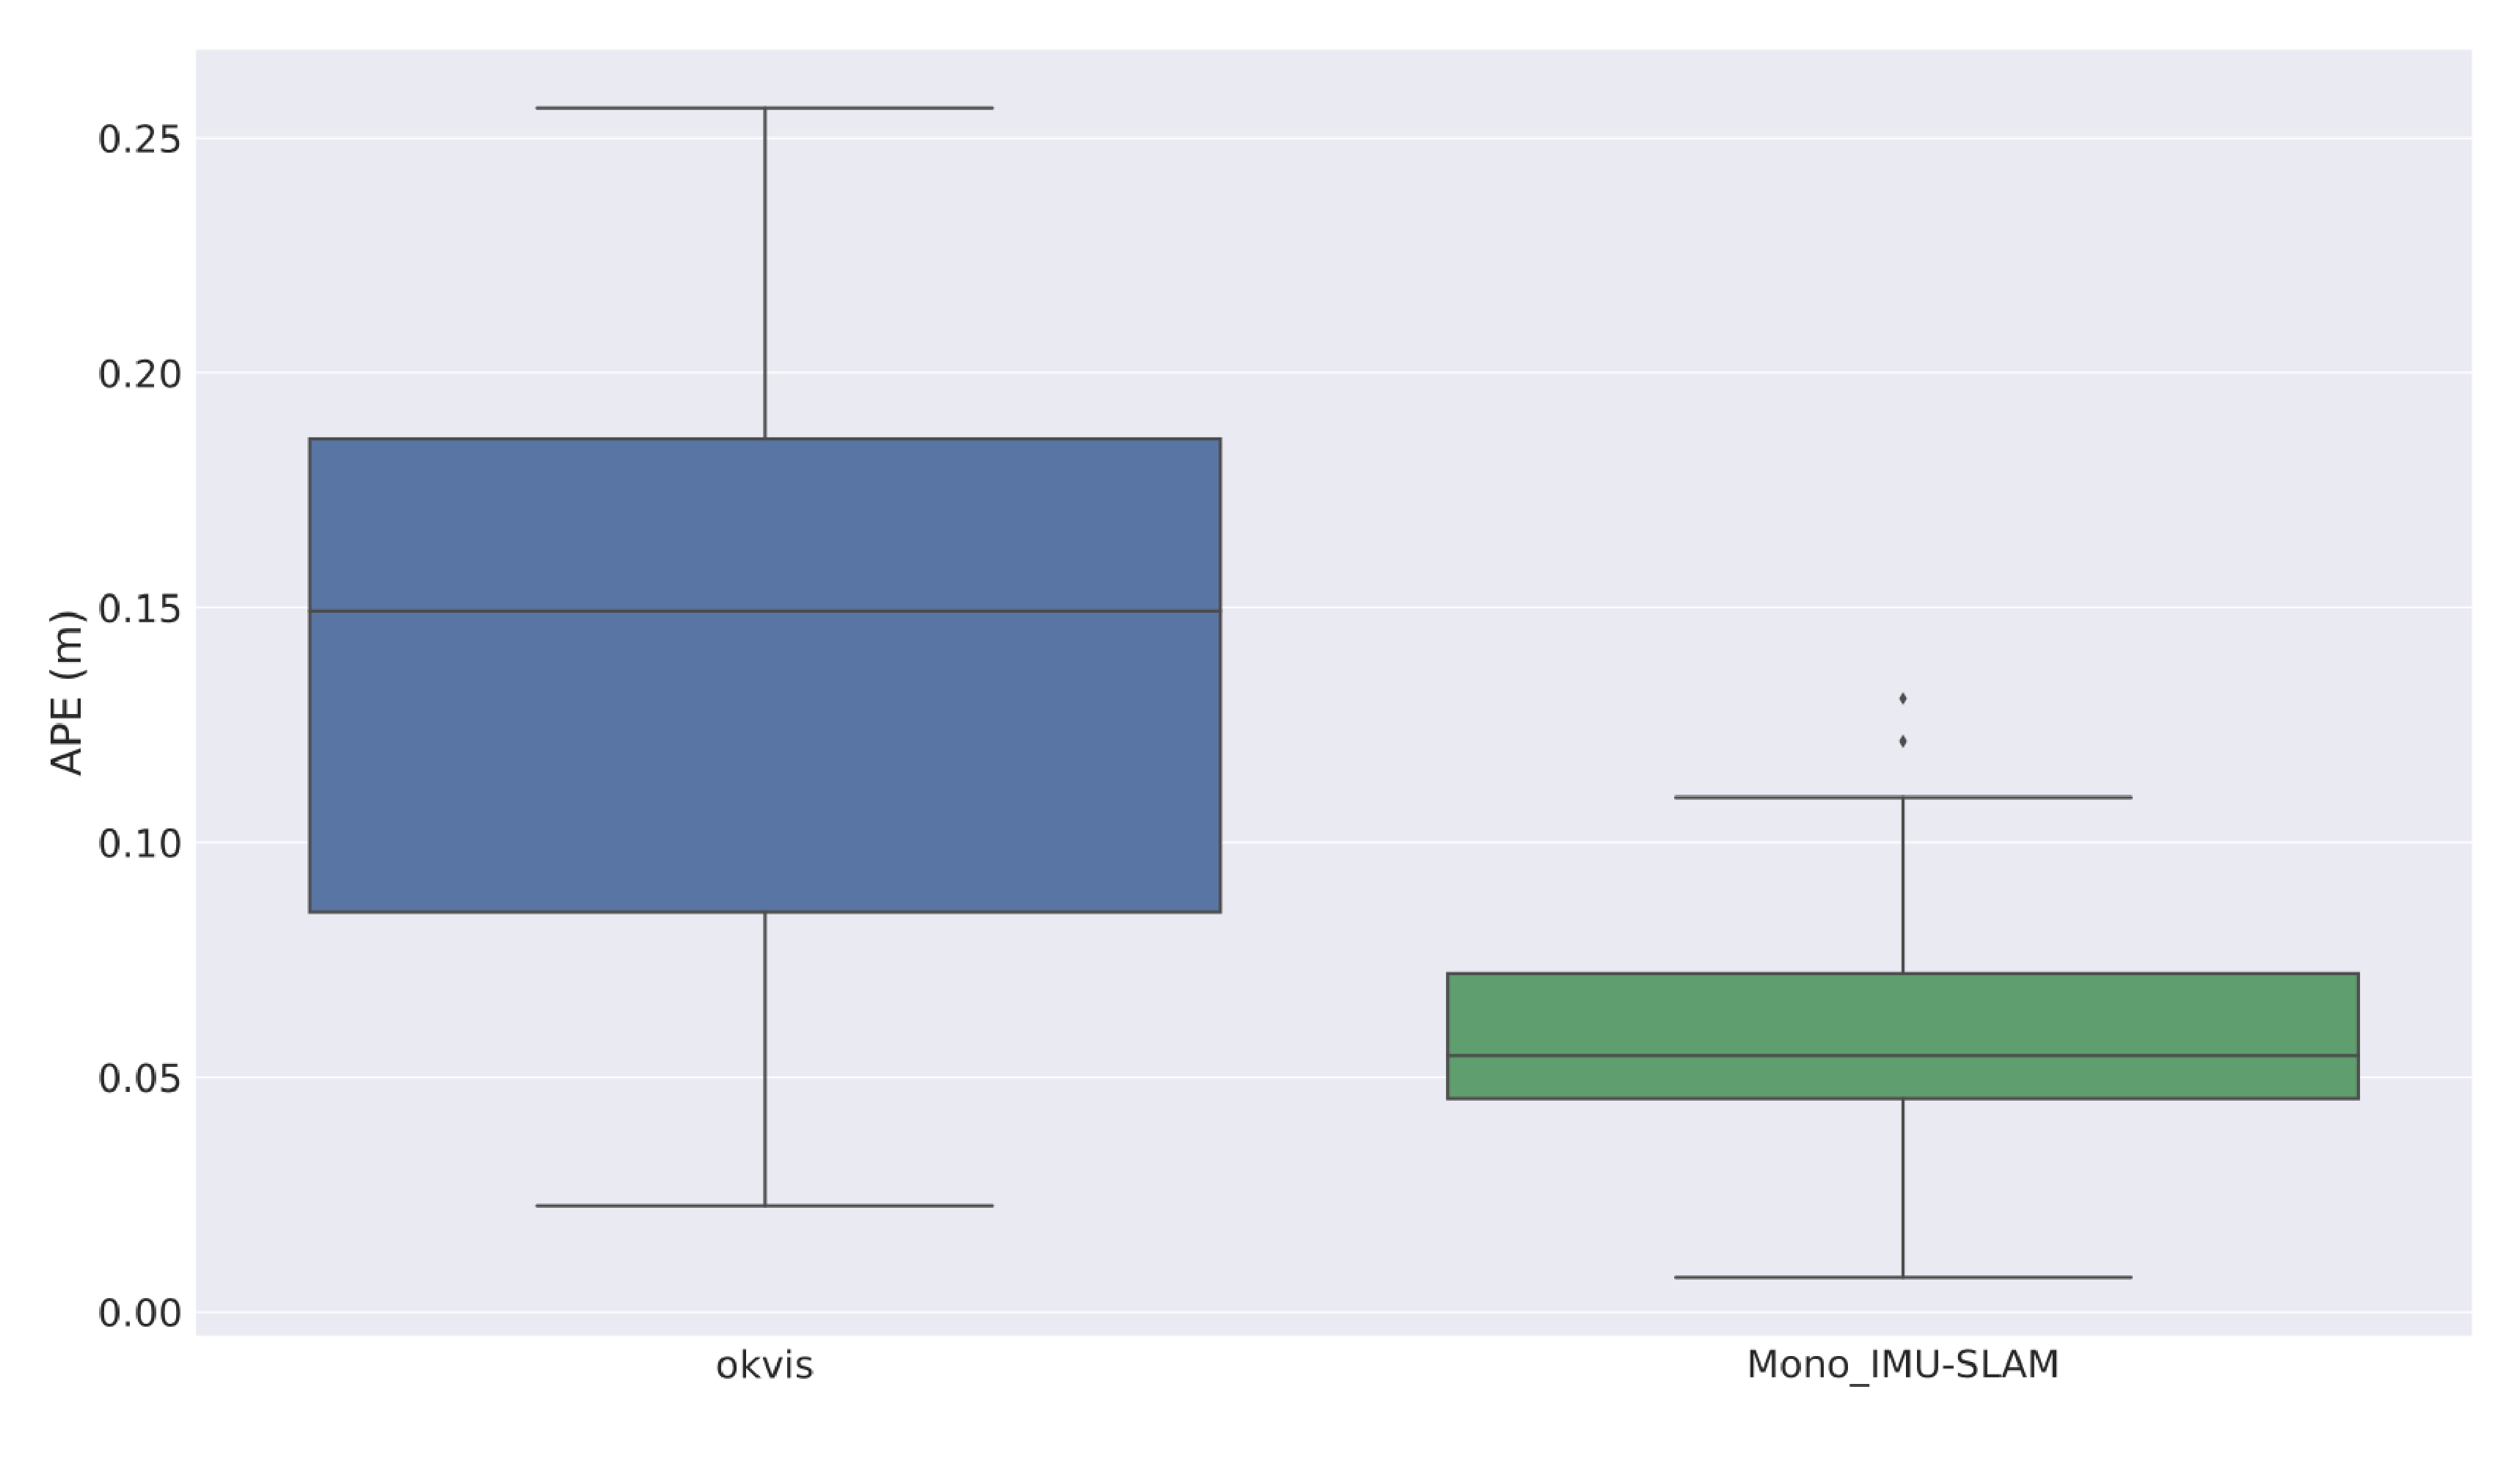
\includegraphics[scale=0.18,angle=-90]{figures/Fig5-4_a.pdf}                    
          }
          \subfigure[]
       	  {
       	  \label{fig5.4-b}
       	  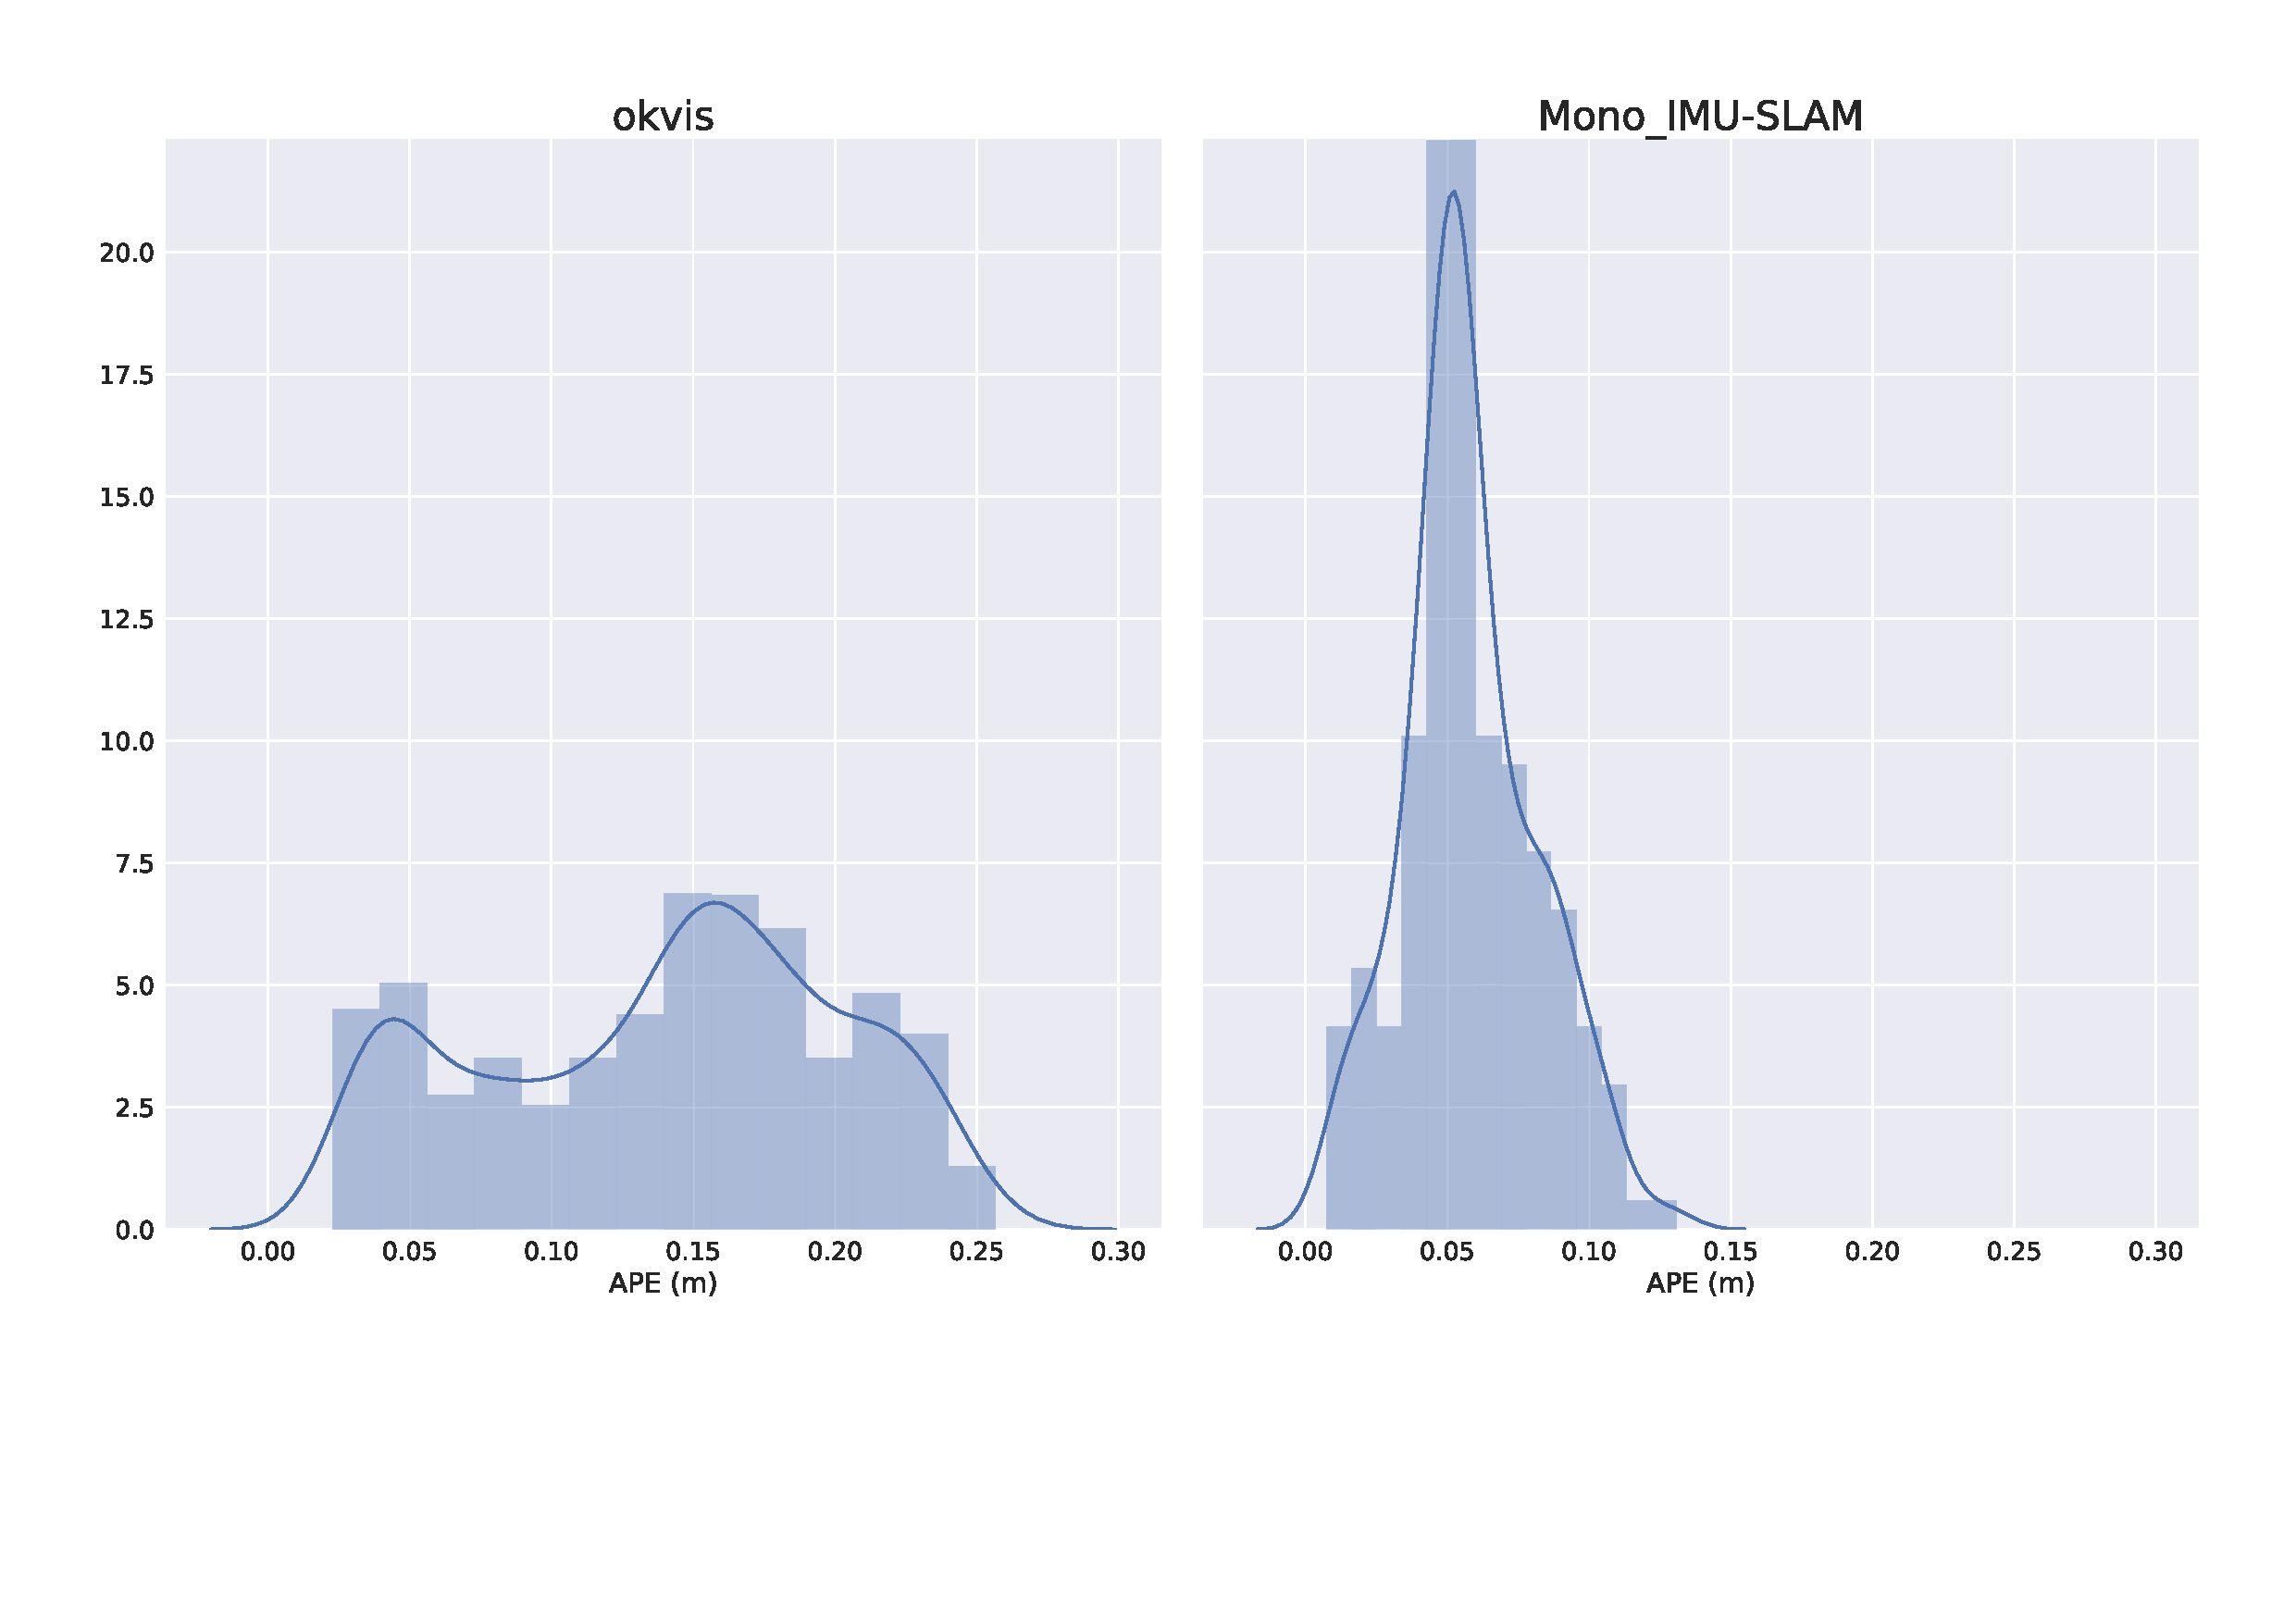
\includegraphics[scale=0.18,angle=-90]{figures/Fig5-4_b.pdf} 
          }  
     \caption{与OKVIS定位精度比较}
\label{fig5.4}
\end{figure}   



\section{本章小结}
本章研究基于IMU预积分的惯性-视觉单目SLAM算法,在传统基于特征的单目算法基础上,利用预积分算法对IMU数据进行处理,将IMU观测模型表示为状态变量的函数与观测噪声和的形式,通过单目SLAM后端非线性优化与IMU进行数据融合。实验表明,本章研究的惯性-视觉单目SLAM算法在IMU初始化阶段可以准确估计运动轨迹尺度和传感器偏移,定位精度高;IMU先验运动信息还可加速特征跟踪和匹配,提高算法鲁棒性。





%\include{chapters/chapter6}

%%==================================================
%% conclusion.tex for BIT Master Thesis
%% modified by yang yating
%% version: 0.1
%% last update: Dec 25th, 2016

%% modified by Meng Chao
%% version: 0.2
%% last update: May 29th, 2017
%%==================================================


\begin{conclusion}
为解决无人机自主飞行的导航定位问题,本文围绕单目视觉SLAM进行研究,从算法和功能上对原有基于特征的单目SLAM进行改进和拓展。特别的,借鉴基于直接法SLAM和多传感器融合领域的研究成果,对基于特征的单目SLAM算法进行改进和完善,取得了较好的效果。本文主要研究成果如下:
\begin{enumerate}  [label={(\arabic*)}]
\iffalse
\item 介绍多旋翼无人机导航定位算法发展,详细综述视觉SLAM的流程和核心算法。对视觉SLAM的理论和算法发展进行了总结,对比单目、双目和RGB-D三种传感器特点。结合国内外视觉SLAM的发展现状和发展趋势,本文认为,就算法角度来看,单目视觉SLAM算法未来的发展方向是半稠密程度以上的环境地图重建,从而提供更为丰富的环境信息;从应用层面出发,单目SLAM可与IMU、GPS和激光雷达等多传感器进行数据融合,提供准确的尺度信息,改善单目SLAM鲁棒性。本文的改进工作主要围绕以上两点展开。
\item 针对特定的对象,研究多旋翼无人机的数学模型和控制率设计。完成无人机的动力学和运动学建模,并对非线性部分进行线性化简。根据经典控制理论,设计串级PID控制器控制无人机的位置和姿态。通过MATLAB仿真,验证无人机数学模型的准确性和控制率的可行性,了解其运动特性,便于后续选择适合用于无人机导航定位的单目SLAM算法。
\fi
\item 详细介绍了单目视觉SLAM的算法框架、理论原理和分类。从定位精度、鲁棒性和地图重构三个方面系统的比较了基于直接法的LSD-SLAM和基于特征的ORB-SLAM。相比于LSD-SLAM,基于特征的ORB-SLAM具有较好的视角不变性和光度不变性,可以在宽基线下稳定跟踪,对于快速运动具有较好的鲁棒性,适宜作为无人机的导航定位系统。但ORB-SLAM也存在一些问题,如重构地图稀疏,无法用于避障和路径规划;单目相机无法获取深度信息,运动轨迹和地图尺度不确定。
\item 针对基于特征的SLAM地图稀疏的问题,研究一种基于特征的单目半稠密SLAM算法。该算法参考直接法SLAM重构原理,采用像素块匹配和基于概率的逆深度假设进行半稠密重构。针对宽基线下的像素块匹配离群值较多的问题,引入逆深度一致性检剔除离群值,提高半稠密地图重构效果。实验表明改进后的基于特征的单目半稠密SLAM算法定位精度高,重构的环境半稠密地图可以满足无人机避障与路径规划的需要。
\item 针对单目SLAM尺度不确定的问题,研究基于IMU预积分的惯性-视觉SLAM算法,在传统基于特征的SLAM基础上,通过预积分算法对IMU数据进行处理,将IMU测量模型表示成状态变量的函数与观测噪声和的形式,通过视觉SLAM后端非线性优化与IMU进行数据融合。实验表明,基于IMU预积分的惯性-视觉SLAM算法可以准确估计运动轨迹的尺度和传感器偏移,算法定位精度高;IMU先验运动信息还可加速特征跟踪和匹配,提高算法鲁棒性。
\end{enumerate}

针对以上研究成果和结论,本文对用于多旋翼无人机导航定位的单目SLAM算法进行了深入研究与全面分析。但由于时间有限,能力欠缺,仍存在一些不足,后续工作可针对以下几个方面深入展开:
\begin{enumerate}  [label={(\arabic*)}]
\item 本文研究的单目半稠密重建只使用CPU处理,因而图像分辨率和帧率均受到限制。可考虑采用GPU加速的方法进行环境重构,可提高运算效率,增加地图稠密程度。
\item 当前针对惯性-视觉SLAM的初始化没有公认的判定方法确定初始化的准确性,后续可考虑结合线性方程的条件数研究自动判定准则,确定初始化状态变量的准确性。
\item 本文分别对单目半稠密重建和惯性-视觉SLAM问题进行研究,由于时间有限,没有将本文的两部分研究成果纳入到一个系统框架中。之后的工作可考虑将两部分算法进行整合,研究一种基于单目的半稠密惯性-视觉SLAM算法,应用于无人机导航定位。
\end{enumerate}





\end{conclusion}



%% 参考文献,五号字,使用 BibTeX,包含参考文献文件.bib

%\bibliography{reference/chap1,reference/chap2} %多个章节的参考文献
\bibliography{reference/ref}


%%%%%%%%%%%%%%%%%%%%%%%%%%%%%%
%% 后置部分
%%%%%%%%%%%%%%%%%%%%%%%%%%%%%%

%% 附录(章节编号重新计算,使用字母进行编号)
\appendix
\renewcommand\theequation{\Alph{chapter}--\arabic{equation}}  % 附录中编号形式是"A-1"的样子
\renewcommand\thefigure{\Alph{chapter}--\arabic{figure}}
\renewcommand\thetable{\Alph{chapter}--\arabic{table}}

%%==================================================
%% app1.tex for BIT Master Thesis
%% modified by yang yating
%% version: 0.1
%% last update: Dec 25th, 2016

%% modified by Meng Chao
%% version: 0.2
%% last update: May 29th, 2017
%%==================================================


\chapter{IMU预积分中的数学原理}

\section*{李群与李代数性质}

李群中的特殊正交群$SO(3) \doteq \{ \boldsymbol{R} \in \mathds{R}^{3 \times 3}:\ \boldsymbol{R}^T \boldsymbol{R}=\boldsymbol{I},det(\boldsymbol{R})=\boldsymbol{I} \}$表示刚体在三维空间的旋转矩阵,李群$SO(3)$在流型空间上单位元素处的正切为李代数$\mathfrak{so}(3) \doteq \{ \boldsymbol{\phi}: \boldsymbol{\phi} \in  \mathds{R}^3  \}$。
李代数可以通过指数映射$\exp(\cdot)$与李群相关联,有
\begin{equation}
\label{equ1}
\boldsymbol{R} = \exp \left( \boldsymbol{\phi}^\wedge \right) = \boldsymbol{I}+{ \sin( \Vert \boldsymbol{\phi} \Vert) \over \Vert \boldsymbol{\phi} \Vert } \boldsymbol{\phi}^{\wedge} + { {1-\cos(\Vert \boldsymbol{\phi} \Vert)} \over \Vert \boldsymbol{\phi} \Vert^2 }\left(\boldsymbol{\phi}^{\wedge}\right)^2
\end{equation}
其中$(\cdot)^\wedge$表示向量的反对称矩阵,反对称矩阵具有如下性质。
\begin{equation}
\boldsymbol{a}^\wedge \boldsymbol{b} = - \boldsymbol{b}^\wedge \boldsymbol{a} \ \ \ \forall \boldsymbol{a},\boldsymbol{b} \in \mathds{R}^3
\end{equation}
李群也可通过对数映射$\log(\cdot)$与李代数相关联,设$\boldsymbol{\phi} = \boldsymbol{a} \varphi$
\begin{equation}
\label{equ2}
\begin{aligned}
\boldsymbol{\phi} &= \log(\boldsymbol{R}) = { \varphi \cdot \left(\boldsymbol{R} - \boldsymbol{R}^T \right)  \over 2 \sin(\varphi) }
\\
\varphi &= \cos^{-1} \left( tr(\boldsymbol{R})-1 \over 2 \right)
\end{aligned}
\end{equation}
李代数到李群的指数映射泰勒展开的一阶近似可以表示为
\begin{equation}
\label{equ3}
\begin{aligned}
\exp\left( \boldsymbol{\phi}^{\wedge} \right) & \approx  \boldsymbol{I} + \boldsymbol{\phi}^{\wedge}
\\
\exp\left( \boldsymbol{\phi}^{\wedge} + \delta\boldsymbol{\phi}^{\wedge}  \right) & \approx \exp \left( \boldsymbol{\phi}^{\wedge} \right)  \exp \left( J_r\left( \boldsymbol{\phi} \right) \delta\boldsymbol{\phi}^{\wedge} \right)
\end{aligned}
\end{equation}
其中$J_r\left( \boldsymbol{\phi} \right)$表示$SO(3)$相对于李代数微小增量的右雅各比矩阵
\begin{equation}
\label{equ4}
J_r\left( \boldsymbol{\phi} \right) = \boldsymbol{I} - {{1-\cos(\Vert \boldsymbol{\phi} \Vert)} \over \Vert \boldsymbol{\phi} \Vert^2 } \boldsymbol{\phi}^{\wedge}+
{{ \Vert \boldsymbol{\phi} \Vert-\sin(\Vert \boldsymbol{\phi} \Vert)} \over \Vert \boldsymbol{\phi^3} \Vert }\left(\boldsymbol{\phi}^{\wedge}\right)^2
\end{equation}
李代数指数映射与李群的乘积有以下性质
\begin{equation}
\label{equ5}
\begin{aligned}
\boldsymbol{R} \exp \left( \boldsymbol{\phi} \right) \boldsymbol{R}^T &= \exp \left( \boldsymbol{R}  \boldsymbol{\phi}^{\wedge} \boldsymbol{R}^T \right) = \exp \left(  \boldsymbol{R} \boldsymbol{\phi} \right)
\\ 
\Leftrightarrow \ \ \ \exp \left( \boldsymbol{\phi} \right) \boldsymbol{R} &=  \boldsymbol{R} \exp \left(\left( \boldsymbol{R}^T  \boldsymbol{\phi} \right)^\wedge\right)
\end{aligned}
\end{equation}

 % 更新记录
\include{chapters/app2} 
%%==================================================
%% app1.tex for BIT Master Thesis
%% modified by yang yating
%% version: 0.1
%% last update: Dec 25th, 2016

%% modified by Meng Chao
%% version: 0.2
%% last update: May 29th, 2017
%%==================================================


\chapter{单目数据集场景}
\label{DataSets}


\begin{figure}[h]
\centering
	\subfigure[fr2/desk场景]
    {
		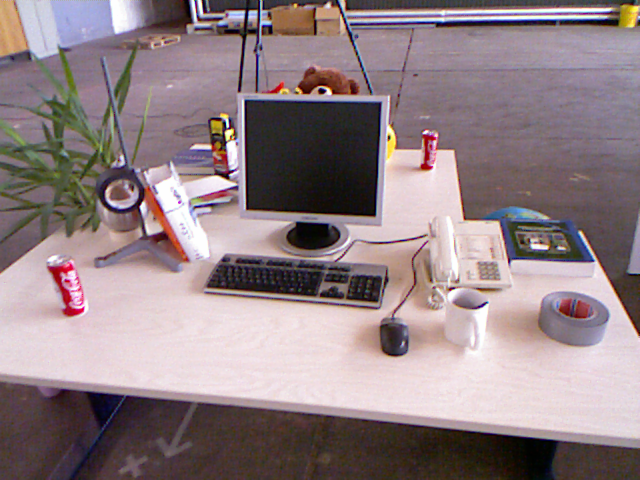
\includegraphics[scale=0.27]{figures/fr2_desk.png}  
	}
	\subfigure[fr3/nostructure\_ texture\_ near\_ with\_ loop场景]
    {	
		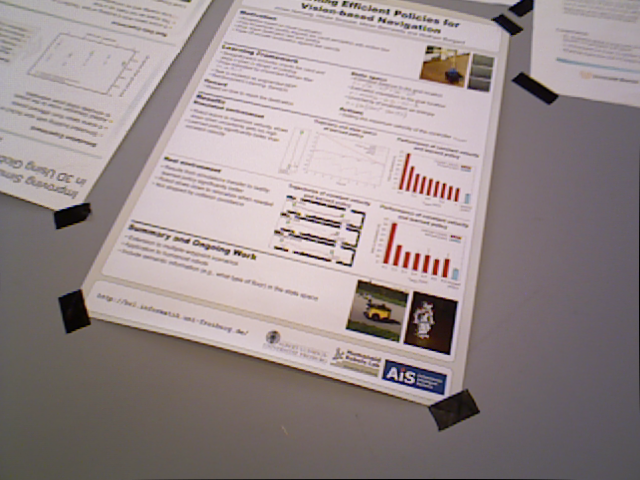
\includegraphics[scale=0.27]{figures/fr3_nostructure.png}
	}
	\subfigure[fr3/long\_ office\_ household场景]
    {	
		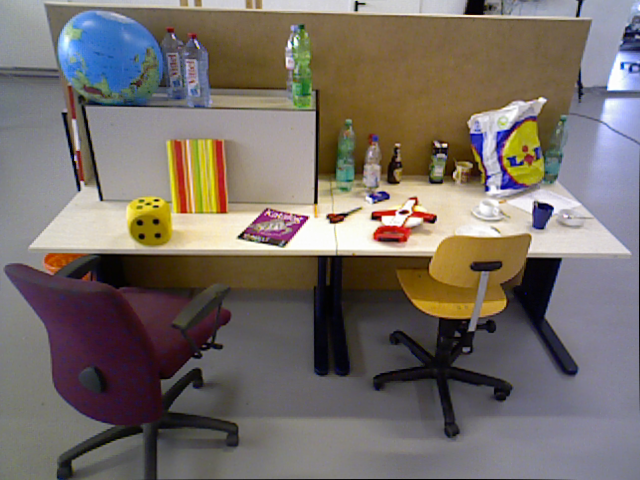
\includegraphics[scale=0.27]{figures/fr3_long_office.png}
	}
\caption{TUM RGBD数据集}
\end{figure}


\begin{figure}[h]
\centering
	\subfigure[MH场景]
    {
		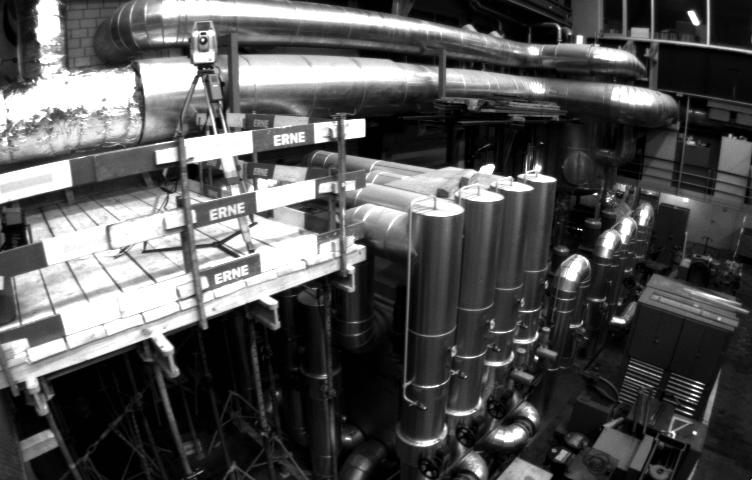
\includegraphics[scale=0.25]{figures/MH.png}  
	}
	\subfigure[V1场景]
    {	
		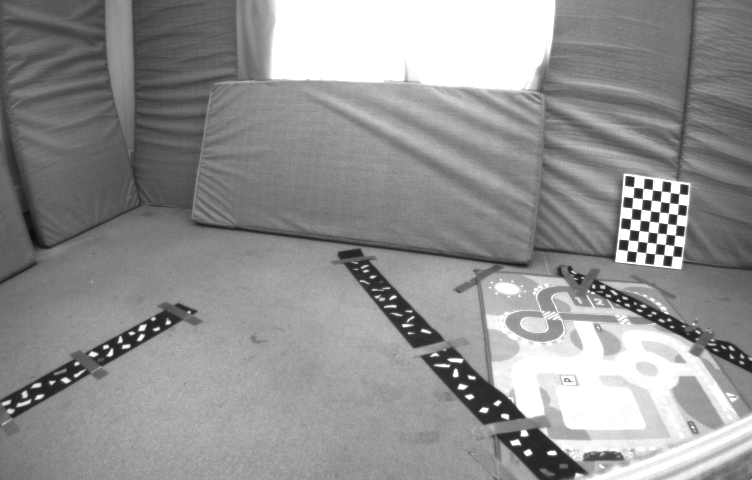
\includegraphics[scale=0.25]{figures/V1.png}
	}
\caption{EuRoC数据集}
\end{figure}





 
%(其后部分无编号)
\backmatter

% 发表文章目录
%%==================================================
%% pub.tex for BIT Master Thesis
%% modified by yang yating
%% version: 0.1
%% last update: Dec 25th, 2016

%% modified by Meng Chao
%% version: 0.2
%% last update: May 29th, 2017
%%==================================================

\begin{publications}{99}

	\item\textsc{Chao Meng,Baiwei Guo,Xin Liu}. {Simultaneous localization and mapping using monocular direct method}[C]. Control, Automation, Robotics and Vision (ICARCV), 2016 14th International Conference on, IEEE, 2016: 1-5.(EI检索)
	
      
	\item\textsc{Xin Liu,Baiwei Guo,Chao Meng}. {A Method of Simultaneous Location and Mapping Based on RGBD Cameras}[C]. Control, Automation, Robotics and Vision (ICARCV), 2016 14th International Conference on, IEEE, 2016: 1-5.(EI检索)

    
\end{publications}
% 致谢
%%==================================================
%% thanks.tex for BIT Master Thesis
%% modified by yang yating
%% version: 0.1
%% last update: Dec 25th, 2016

%% modified by Meng Chao
%% version: 0.2
%% last update: May 29th, 2017
%%==================================================

\begin{thanks}


感谢我的导师郭百巍老师!本论文的工作是在郭百巍老师的指导下完成的。在北京理工大学攻读硕士学位期间,无论在学习、科研还是生活上,郭老师都给予了我很多的的指导和帮助,提出许多十分有价值的想法和建议。郭老师科学严谨的治学态度、踏实勤奋的工作作风、渊博的知识,为我树立了学习的榜样,使我获益匪浅。在此,我向郭百巍老师表达由衷的感谢和敬意。

感谢实验室的师兄师姐师弟们,正是实验室浓厚的科研氛围熏陶了我,实验室的生活让我感受到集体大家庭的温暖。另外感谢宿舍的舍友在生活上的关心与照顾。在此,特别感谢徐勇老师、赵良玉老师、宋晓东老师、单家元老师、孟秀云老师、丁艳老师、王彦恺老师、张卫忠老师,在攻读硕士学位期间,课题组的老师们为我在科研工作上提供了思路,给予了我很大的帮助。

此外,感谢我的室友司维勇、王文彤、胡琛等人,陪着我度过了这一段美好的时光。希望我们会永远记得在北理的回忆。

感谢我的父母家人和女朋友,感谢你们无微不至的关怀与鼓励。正是你们在背后默默的支持和奉献才能使我顺利完成学业。


\end{thanks}

% 作者简介(博士论文需要)
%\include{chapters/resume}


\end{document}
